\part{A Crush Course on CFT}
% 计数器清零,每个part都要引用,除了part1
\setcounter{theorem}{0}
\setcounter{definition}{0}
\setcounter{lemma}{0}
\setcounter{sidenote}{1}

CFT经典教材是大黄书\cite{DiFrancesco:1997nk},教材\cite{Blumenhagen:2009zz,ito}也是不错的选择\sn{伊藤克司先生的书还没有官方中文译本,不过这里有民间译本的重排本\url{https://github.com/WHUZBF/CFT-book}},还有一些比较好的讲义\cite{Nawata:2022lsw,Ginsparg:1988ui,Qualls:2015qjb},共形场论的自举(bootstrap)方法也是非常重要的,可以见讲义\cite{Ribault:2014hia}的专门介绍。CFT也可以当作一门数学课来学习,偏重于数学的阅读材料有\cite{Schottenloher:2008zz}。

首先是一些Overview性质的介绍。CFT无非就是一种特殊的QFT,但是这个时候理论具有比Poincar\'e对称性更大的对称性,在二维的情况下甚至提升为无穷维的对称性,这种对称性能让我们不通过微扰场论直接确定关联函数。一般的QFT中我们用Poincar\'e的不同的不可约表示来标记不同的场,或者说,我们用自旋来标记场,到了CFT这边,我们还需要使用共形维数$\Delta$来标记,对于$s=0$的标量场,共形维数定义为在Dilation $x\mapsto\lambda x$ 下场变换为:
\begin{equation}
	\phi^\prime(\lambda \vec{x})=\lambda^{-\Delta}\phi(\vec x)
\end{equation}
但是这只是对Dilation要求场在共形变换下“协变”,进一步要求对任意共形变换“协变”就给出了\textbf{初级场}(primary field)的定义。\sn{注意我们遵从大黄书的符号约定,和\cite{Blumenhagen:2009zz,Ginsparg:1988ui}的定义恰巧相反,对最终CFT中的一些结论没有任何影响,仅仅只是中间推导过程有些细微的差别。}\sn{$s=1/2$是何形式?}
\begin{definition}
	共形维数为$\Delta$的初级场(s=0)定义为在任意共形变换下满足:
	\begin{equation}
		\phi^\prime(\vec{x^\prime})=\left|\frac{\partial \vec {x^\prime}}{\partial \vec {x}}\right|^{\Delta/d}\phi(\vec {x})
	\end{equation}
\end{definition}

初级场将是后面研究的主要对象。二维的共形对称性比较特殊,分为global和local的,如果上面的“协变性”只对global的共形变换适用,那我们称之为\textbf{准初级场}(quasi-primary field),显然初级场一定是准初级场,反过来却不一定。二维情况下我们还使用复平面为坐标\footnote{这是欧氏空间CFT的主要选取,也是后文研究的主要内容,Wick转动到闵氏时空之后选取所谓光锥坐标。},但是我们为了一些地方的方便,并不是考虑的$\mathbb{C}$,而是$\mathbb{C}^2$,也就是说我们把$z,\bar z$看作是完全独立的变量,进在一些特殊情况下认为$z^*=\bar z$。而且把$\Delta$拆分为共形权$(h,\bar h)=\frac{1}{2}\left(\Delta+s,\Delta-s\right)$在这一符号约定下,共形权定义变为:
\begin{equation}
	\boxed{
	\phi^{\prime}(\lambda z,\overline{\lambda}\overline{z})=\lambda^{-h}\overline{\lambda}^{-\overline{h}}\phi(z,\overline{z})
	}
\end{equation}
(准)初级场定义变为:
\begin{equation}
	\boxed{
		\phi^{\prime}\left(f(z),\overline{f}(\overline{z})\right)=\left(\frac{\partial f}{\partial z}\right)^{-h}\left(\frac{\partial\overline{f}}{\partial\bar{z}}\right)^{\overline{-h}}\phi(z,\bar{z})
	}
\end{equation}
如果$\phi$全纯我们称为\textbf{chiral},反全纯称为\textbf{anti-chiral}。无穷小共形变换$x\mapsto x+\epsilon$下:
\begin{equation}\label{ict}
	\boxed{
	\delta_{\epsilon,\bar{\epsilon}}\phi(z,\bar{z})\equiv\phi^\prime(x^\prime)-\phi(x)=-\left(h\partial_z\epsilon+\epsilon\partial_z+\overline{h}\partial_{\bar{z}}\bar{\epsilon}+\overline{\epsilon}\partial_{\bar{z}}\right)\phi(z,\overline{z})
	}
\end{equation}
\begin{remark}
	初级场的定义可以看作是一种拓宽的张量定义,考虑一个带$s$个协变指标的张量,在任意坐标变换$x\mapsto x+\epsilon(x)$下:
	\[-\delta\Phi_{\mu_1\cdots\mu_s}=\epsilon^\nu\partial_\nu\Phi_{\mu_1\cdots\mu_s}+(\partial_{\mu_1}\epsilon^\nu)\Phi_{\nu\mu_2\cdots\mu_s}+\cdots+(\partial_{\mu_s}\epsilon^\nu)\Phi_{\mu_1\cdots\mu_{s-1}\nu}\]
	换到复平面,简单起见只考虑全纯部分,那么$h=s$,上面的定义局限于$h$是整数,现在考虑任意取值,那些指标也没必要写出了,便得到:
	\[-\delta\Phi=\epsilon\partial\Phi+s\partial \epsilon\Phi\]
	这就是前面得到的无穷小变换形式。
\end{remark}

同QFT一样,这些场都会量子化成算符。不像QFT中我们研究的场是有限多个的,比如说QED就是正负电子对应的Dirac场和一个U(1)规范场耦合,CFT中我们研究的场很多情况下会是无穷多个的,因为我们把$\phi,\partial\phi$看作是不同的场,因为他们是不同共形权的初级场。定义一个CFT第一步就是告诉我们理论中有哪些初级场,也就是一个\textbf{谱}(Spectrum)$\{\mathcal{O}_{h,\bar h}\}$。CFT中我们并非按照微扰场论那一套来建立关联函数的计算方法的,而会去关注场之间的\textbf{算符乘积展开(OPE)},后面将会看到自举给出了OPE的绝大多数信息,还有一些系数是自举无法确定的,需要CFT的定义给定,这是定义CFT的第二个data。我们这样做是在算符的观点下看问题,或者说是在海森堡表象下看问题,那CFT的态是什么呢?这其实被所谓\textbf{态算符对应}联系起来。

最后想强调一点,正是因为CFT的思考方式和一般的QFT有比较大的不同,所以CFT的建立甚至是不需要已知理论的拉氏量的,我们需要知道的只是理论拥有的对称性,然后去找对称性的表示构造谱,能动量张量则刻画了CFT在共形变换下的性质,是构建OPE必须的,如果强行利用拉格朗日量进行分析反而会变得非常复杂,有的CFT甚至是没办法写下一个拉氏量的,但是通过自洽性分析我们是知道这种理论的存在性的,而且可以根据自举方法走得很远。

\section{Virasoro Algebra}
讨论共形场论,都是在量子层面上已经消去共形反常后的理论,比如YM理论就是量子化后存在共形反常的QFT,从而不能看作一个CFT。二维CFT的共形代数是$\mathrm{Witt}\times\overline{\mathrm{Witt}}$,后面我们讨论CFT其实都是在其中心扩张$\mathrm{Vir_c}\times\overline{\mathrm{Vir_c}}$下进行\sn{明确一下convention,扩张前的代数用小写$l$标记,扩张后的用大写$L$标记}。这里我不打算讨论过多中心荷的物理意义,这应当是弦论课的内容,为何要引入中心荷可以从群表示的观点来看。

首先如果一个CFT具有某个对称性,这个对称性构成了一个群,那么体系的谱就生活在这个群的群表示之中\sn{严格说是表示的最高权是那些初级场,也就是CFT的谱,由这些谱生成的次级态最终张成整个CFT的希尔伯特空间,也就是对称代数的表示。}。也就是说假设对称代数为$\mathfrak{V}\times\bar{\mathfrak{V}}$\sn{注意在二维CFT中我们都会将对称代数复化为两个独立的部分。两个独立的李代数可以作为线性空间考虑他们的直和$\mathfrak{V}\oplus\bar{\mathfrak{V}}$,这里写成$\times$也没错,是将他们考虑成集合,然后做卡氏积,由于两部分独立,所以这两者本质上没区别。},则:
\begin{equation}
	\boxed{\mathcal{S}=\bigoplus_{(\mathcal{R},\mathcal{R}^{\prime})\in\mathrm{Rep}(\mathfrak{V})^2}m_{\mathcal{R},\mathcal{R}^{\prime}}\mathcal{R}\otimes\bar{\mathcal{R}^{\prime}}}
\end{equation}
但是这个表示只需要是个射影表示就好,而射影表示对应的是李代数的中心扩张的表示。前面处理洛伦兹群我们不用考虑那么多,因为我们这证明了理论总是可以redefine来消去中心荷,但是一般的共形场论至少都有Virasoro对称性,而这个代数的中心荷是non-trivial的,一般是不能消除的,所以我们考虑对称性并非直接考虑$\mathrm{Vir}$,而是$\mathrm{Vir}_c$。
\begin{theorem}[Virasoro Algebra]
	\begin{equation}
		\boxed{
		\left[L_m,L_n\right]=\left(m-n\right)L_{m+n}+\frac c{12}\left(m^3-m\right)\delta_{m+n,0}
		}
	\end{equation}
\end{theorem}
\begin{remark}
	如果我们考虑$\mathfrak{sl}(2,\mathbbm{C})$子代数,会发现中心扩张是trivial的。
\end{remark}
\section{Radial Quantization and Hilbert Space}
\subsection{Radial Quantization}
对于$1+1$维时空,可以把空间方向一点紧化为圆,这样平面就会变为一个圆柱面,这样就可以引入圆柱面上的复坐标$w=x^0+ix^1$,这样$w\sim w+2\pi i$自动满足周期性条件,这也是弦论worldsheet的图像。而圆柱面又可以通过共形变换$w\mapsto e^w$变到另一个复平面上:
\begin{figure}[htbp]
	\centering
	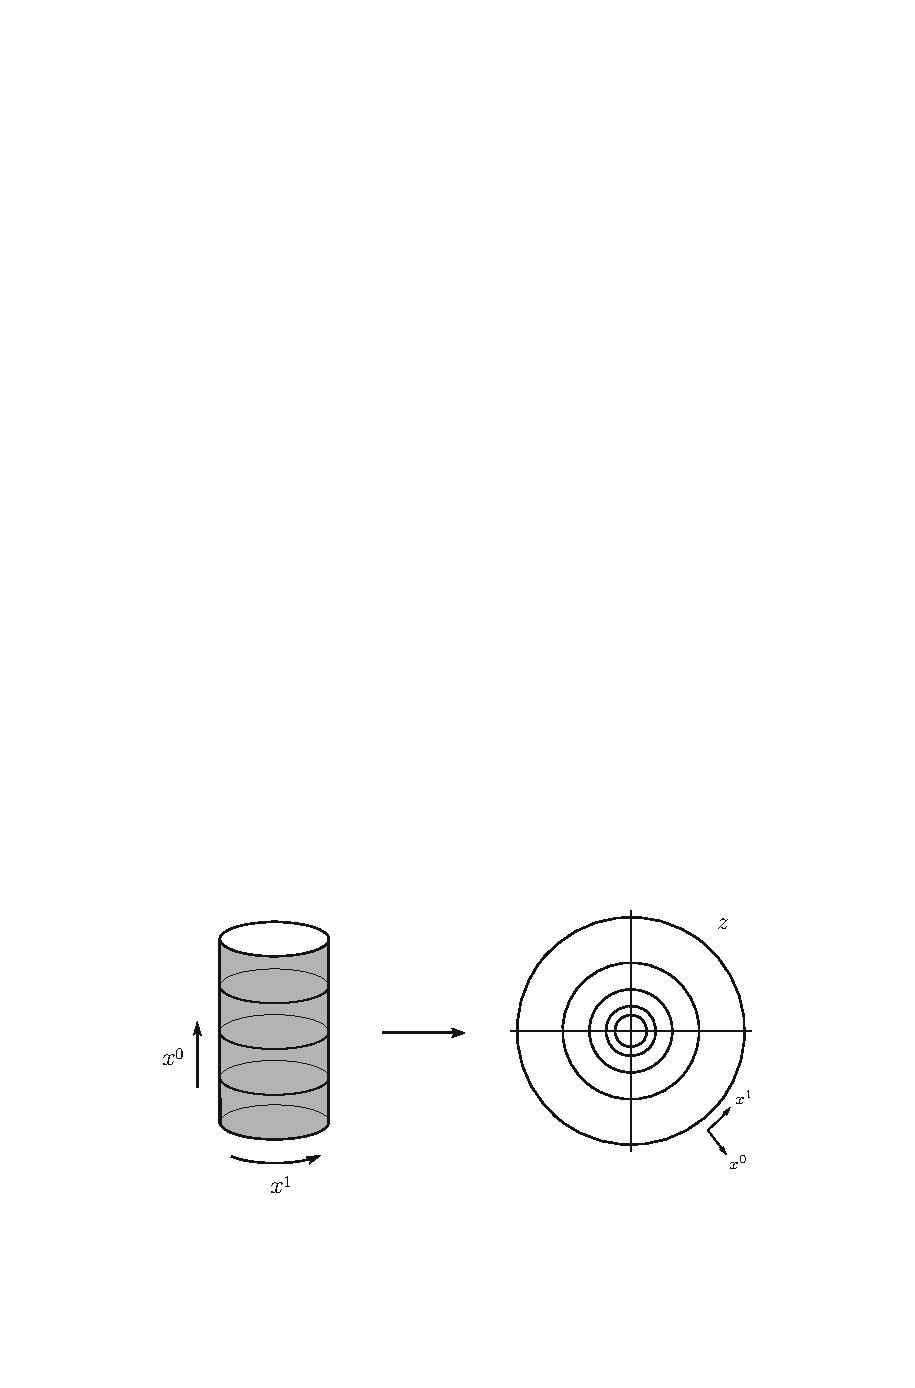
\includegraphics{figs/fig9.pdf}
	\caption{径向量子化}
\end{figure}
在这一变换下,时间方向变为了径向,空间方向变成了角向,而且把整个无穷远映射到了原点这一个点上。这下时间平移对应的哈密顿量$H$到复平面这边就变成了dilation算子$D$,而空间平移对应旋转$e^{i\theta}$:
\begin{equation}
		\boxed{H=L_0+\bar {L}_0,\quad P=i\left(L_0-\bar {L}_0\right)}
\end{equation}
也正是因为时间方向变成了径向,时序积就应当变成“径向顺序积”,我们要去计算的就是径向顺序积的真空期望值,对于玻色子定义为:\sn{费米子把下面的情况改成负号就好}
\begin{equation}
	R\bigl(A(z)B(w)\bigr)\equiv\begin{cases}{}A(z)B(w)&\text{for }|z|>|w|,\\B(w)A(z)&\text{for }|w|>|z|.\end{cases}
\end{equation}

圆柱上的场我们用$\varphi(w,\bar w)$表示,复平面上的场用$\phi(z,\bar z)$表示,那么根据共形变换:
\begin{equation}
	\phi(z,\bar z)=z^{-h}{\bar {z}}^{-\bar h}\varphi(w,\bar w)
\end{equation}
在圆柱那边的CFT中我们知道$\varphi(w,\bar w)$可以做平面波展开为$e^{-ip^0x^0+ip^1x^1}$,由于我们考虑的是欧氏空间的场论,Wick转动后得到$e^{-p^0x^0+ip^1x^1}$,即$(e^{-w})^n(e^{-\bar w})^{\bar m}$的形式\sn{$n+m=p^0,n-m=p^1$}。而这恰恰就是洛朗展开的每一项!所以复平面上的CFT的模式展开为洛朗展开:
\begin{theorem}[Mode Expansion]
	\begin{equation}
		\boxed{\phi(z,\overline{z})=\sum_{n,\overline{m}\in\mathbb{Z}}z^{-n-h}\overline{z}^{-\overline{m}-\overline{h}}\phi_{n,\overline{m}}}
	\end{equation}
\end{theorem}
量子化场就是把$\phi_{n,\bar m}$量子化为算符,这些算符具有$(n,\bar m)$的权。

QFT微扰计算中一个非常重要的概念是渐近态,我们考虑的都是无穷远处的平面波入射经过复杂的相互作用后的平面波出射,微扰的角度看入射态就是在无穷远处的过去在真空附近施加一个扰动,也就是插入场算符,出射态也类似的这样做,这样就会自然出来时序积,然后LSZ约化这些的去计算振幅。同样的CFT这边也有这样的物理图景,只是现在无穷远处过去被映射到原点这一个点上了,所以渐近态应该定义为:
\begin{equation}
	\ket{\phi}=\lim_{z,\overline{z}\to0}\phi(z,\overline{z})\ket{0}
\end{equation}
在原点处上式不奇异自然要求:\sn{这似乎告诉我们$n>-h,\bar m>-\bar h$对应的是CFT中的湮灭算符,后面讲到对易子会回到这里}
\begin{equation}\label{eq:30.6}
	\phi_{n,\overline{m}}\ket{0} =0\quad\text{for}\quad n>-h,\quad\overline{m}>-\overline{h}
\end{equation}
完整得到渐近态的公式:
\begin{equation}
	\boxed{|\phi\rangle=\lim\limits_{z,\overline{z}\to0}\phi(z,\overline{z})\left|0\right\rangle=\phi_{-h,-\overline{h}}\left|0\right\rangle}
\end{equation}
这里有个非常有趣的地方,本来一个算符里面有很多模,最后只剩下了一个,所以在CFT中,态和\textbf{局域}算符是唯一对应的!这就是态\mbox{-}算符对应。这和一般的QFT形成了鲜明的对比,那里一个场对应是不同“方向”平面波的组合,没有做到一一对应,但是CFT做到正是因为他把一个无穷大的空间部分在无穷远的过去全部紧化到了原点这一处,为了加深理解我们用路径积分的观点来看一下。

回忆量子力学中的传播子可以用路径积分表达为:
\begin{equation}
	G(x_f,x_i)=\int_{x(\tau_i)=x_i}^{x(\tau_f)=x_f}\mathcal{D}xe^{iS}
\end{equation}
那么演化后的末态波函数可以用初态波函数传播得到:
\begin{equation}
	\psi_{f}(x_{f},\tau_{f})=\int dx_{i}G(x_{f},x_{i})\psi_{i}(x_{i},\tau_{i})
\end{equation}
QFT这边“波函数”是一个泛函$\Psi[\phi(\sigma)]$,其模方表示在固定时间,空间中每个点$\sigma$上出现场构型$\phi(\sigma)$的概率,可以用路径积分得到末态:
\begin{equation}
	\Psi_f[\phi_f(\sigma),\tau_f]=\int\mathcal{D}\phi_i\int_{\phi(\tau_i)=\phi_i}^{\phi(\tau_f)=\phi_f}\mathcal{D}\phi e^{-S[\phi]}\Psi_i[\phi_i(\sigma),\tau_i]
\end{equation}
现在从柱面换到复平面CFT:
\begin{equation}
	\Psi_f[\phi_f(\sigma),r_f]=\int\mathcal{D}\phi_i\int_{\phi(r_i)=\phi_i}^{\phi(r_f)=\phi_f}\mathcal{D}\phi e^{-S[\phi]}\Psi_i[\phi_i(\sigma),r_i]
\end{equation}
不难发现初始态的作用是对$|z|=r_i$的积分进行加权,构造初始态需要在无穷远的过去,$r_i\to 0$,从而初始态只对原点处积分进行加权,等价于在原点处插入一个算子,即:
\begin{equation}
	\Psi[\phi_f;r]=\int^{\phi(r)=\phi_f}\mathcal{D}\phi e^{-S[\phi]}\mathcal{O}(z=0)
\end{equation}

\subsection{BPZ Conjugate}
为了构建关联函数,我们需要“左矢”,也就是厄米共轭来构造出射态从而有内积,这里谈的BPZ共轭是厄米共轭在Wick转动后的径向量子化欧氏空间CFT上的自然推广。不想扯过多物理上的考量,\cite{ito}从Wick转动后厄米共轭必须与时间反演一同定义BPZ共轭来解释了这一定义。
\begin{definition}[BPZ Conjugate]
	\begin{equation}
		\phi^\dagger(z,\overline{z})=\overline{z}^{-2h}z^{-2\overline{h}}\phi\left(\frac{1}{\overline{z}},\frac{1}{z}\right)
	\end{equation}
\end{definition}
另一方面直接从洛朗展开得到:
\begin{equation}
	\phi^{\dagger}(z,\overline{z})=\overline{z}^{-2h}z^{-2\overline{h}}\sum_{n,\overline{m}\in\mathbb{Z}}\overline{z}^{+n+h}z^{+\overline{m}+\overline{h}}\phi_{n,\overline{m}}=\sum_{n,\overline{m}\in\mathbb{Z}}\overline{z}^{+n-h}z^{+\overline{m}-\overline{h}}\phi_{n,\overline{m}}
\end{equation}
从而有:
\begin{equation}\label{BPZ}
	\boxed{
	\left(\phi_{n,\overline{m}}\right)^\dagger=\phi_{-n,-\overline{m}}
	}
\end{equation}
根据场的BPZ共轭定义,出射态应该定义为:
\begin{equation}
	\bra{\phi}=\lim\limits_{z,\overline{z}\to0}\bra{ 0  }              \phi^\dagger(z,\overline{z})=\lim\limits_{\overline{w},w\to\infty}w^{2h}\overline{w}^{2\overline{h}}\bra{0}\phi(w,\overline{w})=\bra{0}\phi_{h,\bar h}
\end{equation}
这里根据非奇异性要求了:
\begin{equation}\label{eq:30.17}
	\left<0\right|\phi_{n,\overline{m}}=0\quad\text{for}\quad n<h,\quad\overline{m}<\overline{h}
\end{equation}
当然,这里是根据定义严格来构造了一遍,实际计算疯狂使用\ref{BPZ}就好。
\section{Ward Identity and OPE}
\subsection{Infinitesimal Conformal Ward Identity}
前面$\S 4$已经看到共形对称性对应的守恒流可以使用$T_{\mu\nu}\epsilon^\nu$来构造,利用前面得到的最一般的Ward恒等式\ref{eq:19.11},对整个时空进行积分:
\begin{equation}
	\int dx^0dx^1\frac\partial{\partial x^{\mu}} \left\langle j_{a}^{\mu}(x)\Phi(x_{1})\cdots\Phi(x_{n})\right\rangle  =\sum_{i=1}^{n}\left<\Phi(x_{1})\delta_{\epsilon,\bar \epsilon}\cdots\Phi(x_{i})\cdots\Phi(x_{n})\right>
\end{equation}
$z=e^{x^0+ix^1}=x+iy$,进一步利用积分换元得到:\sn{别忘了雅可比行列式}
\begin{equation}
	\begin{aligned}
		\int dx^0dx^1&\partial_\mu\left\langle j_{a}^{\mu}(x)\Phi(x_{1})\cdots\Phi(x_{n})\right\rangle\\
		&=4\int dzd\bar z\left[\bar\partial(T_{\bar z\bar z}\epsilon)+\partial(T_{zz}\bar\epsilon)\right]\\
		&=2\int dxdy\left[\bar\partial(T_{\bar z\bar z}\epsilon)+\partial(T_{zz}\bar\epsilon)\right]
	\end{aligned}
\end{equation}
上面取了约定$\epsilon^z\equiv\epsilon(z),\partial_z\equiv\partial$,反全纯部分类似。现在考虑二元积分的格林公式:
\begin{equation}
	\begin{aligned}\oint_{\partial\Omega}P(x,y)dx+Q(x,y)dy=\int_\Omega dxdy\left(\frac{\partial Q}{\partial x}-\frac{\partial P}{\partial y}\right)\end{aligned}
\end{equation}
利用复变量$z=x+iy$可得下面的形式:\sn{就像是Wick转动一样,我们总假设这样随意复化是可行的}
\begin{equation}
	\begin{aligned}\oint_{\partial_\Omega}frac{1}{2}(P-iQ)dz+\frac{1}{2}(P+iQ)d\bar{z}=\int_\Omega dxdy(\partial(Q-iP)+\bar{\partial}(Q+iP))\end{aligned}
\end{equation}
上式中所有的围道积分都假设方向相对于$z$而言是逆时针,那么在$\bar z$平面上也就是逆时针,不过为了方便,而且CFT中我们也只考虑全纯部分,反全纯部分只要做个Conjugate就好了,后文中$\oint d\bar z$,表示围道方向相对于$\bar z$逆时针。
\begin{equation}
	\int_\Omega dxdy\left(\partial \bar f+\bar\partial f\right)=\frac{1}{2i}\oint_{\partial\omega}fdz+\bar f d\bar z
\end{equation}
再取:
\begin{equation}
	T(z)\equiv-2\pi iT_{zz},\bar T(\bar z)\equiv-2\pi iT_{\bar z\bar z}
\end{equation}
不过这个归一化因子并不重要,只是为了让OPE有一般的convention,后面比如自由玻色子这些具体模型我们都是先将归一化因子待定,再根据OPE的形式来确定它,只需要记住二维共形场论中$T_{zz}$始终全纯,$T_{\bar z\bar z}$始终反全纯就好了。归一化能动张量后,得到初级场的Ward恒等式:
\begin{equation}\label{ward}
	\boxed{
	\sum_{i=1}^{n}\left<\Phi(x_{1})\cdots\delta_{\epsilon,\bar \epsilon}\Phi(x_{i})\cdots\Phi(x_{n})\right>=\frac{1}{2\pi i}\oint\left\langle\left(T(z)\epsilon(z)dz+\bar T(\bar z)\bar \epsilon(\bar z)d\bar z\right)\Phi(x_{1})\cdots\Phi(x_{i})\cdots\Phi(x_{n})\right\rangle
	}
\end{equation}
这里积分围道包围所有$w_i$。根据上式我们可以定义\textbf{Conformal charge}:
\begin{equation}
	Q\equiv\frac{1}{2\pi i}\oint_{\mathcal{C}}\Bigl(dzT(z)\epsilon(z)+d\overline{z}\overline{T}(\overline{z})\overline{\epsilon}(\overline{z})\Bigr)
\end{equation}
这样便有:
\begin{equation}\label{eq:31.9}
	-\delta_{\epsilon,\bar\epsilon}\Phi=\left[Q,\Phi\right]
\end{equation}
\subsection{Operator Product Expansion}
但是\ref{eq:31.9}表面上有个非常大的漏洞,那就是因为全纯,直接导致围道积分始终为0。解决这一问题是注意到Q是一个算符,需要作用到其它场上面,而两个算符靠的非常近时真空涨落发散\sn{类似于$a_p,a_p^\dagger\sim\delta(0)$},上式积分中出现极点。也正是极点的存在导致我们定义局域算符之间的对易子的时候需要做正规化:
\begin{equation}
	[A(z,\bar{z}),B(w,\bar{w})]=\lim_{\begin{smallmatrix}|z|\rightarrow|w|\\|z|>|w|\end{smallmatrix}}A(z,\bar{z})B(w,\bar{w})-\lim_{\begin{smallmatrix}|z|\rightarrow|w|\\|w|>|z|\end{smallmatrix}}B(w,\bar{w})A(z,\bar{z})
\end{equation}
这直接导致对易子的计算可以等价于对径向顺序积的计算:\sn{后文中$\mathcal{C}(w)$表示只绕$w$的逆时针围道}
\begin{equation}
	\boxed{\begin{gathered}
			\oint dz\bigl[A(z),B(w)\bigr] =\oint_{|z|>|w|}dzA(z)B(w)-\oint_{|z|<|w|}dzB(w)A(z) \\
			=\oint_{\mathcal{C}(w)}dzR\Big(A(z)B(w)\Big), 
	\end{gathered}}
\end{equation}
现在利用只含一个初级场的无穷小变换Ward恒等式,或者说\ref{eq:31.9},注意到\ref{ict},以及:\sn{回忆$n$阶极点留数公式:\[\begin{aligned}
		\operatorname{Res}&[f(z),a]\\=&\lim\limits_{z\to a}\frac{1}{(n-1)!}\frac{d^{n-1}}{dz^{n-1}}\left[(z-a)^nf(z)\right]
	\end{aligned}\]}
\begin{equation}\label{eq:31.12}
	\begin{gathered}
		h\left(\partial_{w}\epsilon(w)\right)\phi(w,\overline{w}) =\frac{1}{2\pi i}\oint_{\mathcal{C}(w)}dzh\frac{\epsilon(z)}{(z-w)^{2}}\phi(w,\overline{w}), \\
		\epsilon(w)\left(\partial_{w}\phi(w,\overline{w})\right) =\frac1{2\pi i}\oint_{\mathcal{C}(w)}dz\frac{\epsilon(z)}{z-w}\partial_{w}\phi(w,\overline{w}).
	\end{gathered}
\end{equation}
得到全纯部分:
\begin{equation}
	R\left(T(z)\phi(w,\overline{w})\right)=\frac{h}{(z-w)^2}\phi(w,\overline{w})+\frac{1}{z-w}\partial_w\phi(w,\overline{w})+\ldots 
\end{equation}
\textbf{后面的省略号表示非奇异的项},大多数情况下我们要用的是OPE的奇异部分,因为它完全包含了和对易子一样的信息。像这样的把算符展开成其它算符和的形式称为\textbf{OPE}。在一般的QFT中我们计算时序积需要先写下路径积分,然后进行微扰展开算费曼图,但是CFT中我们只需要去考虑OPE就好了,对称性为我们简化了许多。后面写OPE会省略$R(\cdot)$,利用算符和能动张量之间的OPE我们还能给出一个初级场的等价定义:
\begin{theorem}
	一个场是共形权为$(h,\bar h)$的初级场\textbf{当且仅当}它满足:
	\begin{equation}\label{31.14}
		\boxed{\begin{gathered}
				T(z)\phi(w,\overline{w}) =\frac{h}{(z-w)^{2}}\phi(w,\overline{w})+\frac{1}{z-w}\partial_{w}\phi(w,\overline{w})+\ldots  \\
				\overline{T}(\overline{z})\phi(w,\overline{w}) =\frac{\overline{h}}{(\overline{z}-\overline{w})^{2}}\phi(w,\overline{w})+\frac{1}{\overline{z}-\overline{w}}\partial_{\overline{w}}\phi(w,\overline{w})+\ldots  
		\end{gathered}}
	\end{equation}
\end{theorem}
再次强调,之后写下的所有的OPE都应当认为是在在时序关联函数中插入算符时成立的关系!而且因为是时序积之中的关系:
\begin{equation}
	\langle\mathcal{O}_i(z,\bar{z})\mathcal{O}_j(w,\bar{w})\ldots\rangle=\sum_kC_{ij}^k(z-w,\bar{z}-\bar{w})\langle\mathcal{O}_k(w,\bar{w})\ldots\rangle 
\end{equation}
所以OPE结合律和交换律都自动满足。上式中$\ldots$表示其它任意算符的插入,当然既然是级数总有一个收敛半径,何时OPE的插入是有效的是我们需要关心的,从前面对OPE的推导可以看出我们要求积分围道中只有$w$这一个奇点,所以OPE是精确的当且仅当其它算符的插入点$\{w_i\}$满足$|w-w_i|>|z-w|$。

现在再回到Ward恒等式\ref{ward},但是现在考虑有多个$\Phi$的插入,从前面对OPE的分析得知围道内的极点是$\{w_i\}$,然后利用柯西定理将等式右边的积分换成对绕每个极点的围道积分求和得到:
\begin{equation}
	\begin{aligned}0=\oint\frac{dz}{2\pi i}\epsilon(z)&\Bigg[\Big\langle T(z)\phi_1(w_1,\overline{w}_1)\ldots\phi_N(w_N,\overline{w}_N)\Big\rangle\\
		&-\sum_{i=1}^N\left(\frac{h_i}{(z-w_i)^2}+\frac{1}{z-w_i}\partial_{w_i}\right)\Big\langle\phi_1(w_1,\overline{w}_1)\ldots\phi_N(w_N,\overline{w}_N)\Big\rangle\Bigg]\end{aligned}
\end{equation}
等式左边再次利用\ref{eq:31.12},得到所谓共形Ward恒等式(仅适用于初级场):\sn{注意这并不是代入$T,Phi$之间OPE得到的,因为前面说过OPE收敛半径等于与OPE处最近的其他算符插入处的距离。而我们下面要导出的等式与算符插入点完全无关,推导过程中看到我们将围道变形为单独绕每个$\{w_i\}$的围道来使得OPE的插入是精确的。}
\begin{equation}
	\boxed{\begin{aligned}\big\langle T\left(z\right)&\phi_{1}(w_{1},\overline{w}_{1})\ldots\phi_{N}(w_{N},\overline{w}_{N})\big\rangle\\&=\sum_{i=1}^{N}\left(\frac{h_{i}}{(z-w_{i})^{2}}+\frac{1}{z-w_{i}}\partial_{w_{i}}\right)\Big\langle\phi_{1}(w_{1},\overline{w}_{1})\ldots\phi_{N}(w_{N},\overline{w}_{N})\Big\rangle+\text{regular}\end{aligned}}
\end{equation}
\subsubsection{TT OPE}
CFT$_{2}$中非常重要的OPE是两个能动张量之间的OPE,就平面上的二维共形场论而言,chiral和anti-chiral部分是完全解耦的,所以:
\begin{equation}
	\boxed{
		T(z)\bar T(\bar w)=0
	}
\end{equation}
回忆能动张量$T\sim\frac{\delta S}\delta{g}$,现在来数质量量纲,由于$S$最终要放到指数上,所以$[S]=0$,再根据泛函导数定义$\frac{\delta f(x)}{\delta f(y)}=\delta^D(x-y)$,所以$[f]+\left[\frac{\delta }{\delta f}\right]=[\delta^D]=D$\sn{最后一个等号是因为$\int{dx^D}\delta^D(x-y)=1$,$[x]=-1$}。由于$[g]=0$,所以$[T]=2$,这暗示着在dilation下$T$的共形权为$(2,0)$,根据\ref{31.14}得到:
\begin{equation}
	T(z)T(w)=\cdots+\frac{2T(w)}{(z-w)^2}+\frac{\partial T(w)}{z-w}+\cdots
\end{equation}
第一个省略号是因为$T$不一定是初级场!第二个省略号表示奇异项。但是由于$[TT]=4$,所以最奇异的项只能是$(z-w)^{-4}$,而且分子只能是一个常数,我们取归一化为$c/2$得到:
\begin{theorem}[TT OPE]
	\begin{equation}\label{TT}
		\boxed{
			T(z)T(w)=\frac{c/2}{(z-w)^4}+\frac{2T(w)}{(z-w)^2}+\frac{\partial_wT(w)}{z-w}+\ldots 
		}
	\end{equation}
	$\bar T\bar T$的OPE取个conjugate就好。
\end{theorem}
有两点需要解释一下,首先是为何没有$(z-w)^{-3}$项的加入?这可以解释为由于OPE的交换律,所以$z\leftrightarrow w$对称性会紧闭所有奇数次数项。但是有一个例外是$(z-w)^{-1}$:
\begin{equation}
	\begin{aligned}T(w)T(z)&=\frac{c/2}{(z-w)^4}+\frac{2T(w)+2(z-w)\partial T(w)}{(z-w)^2}-\frac{\partial T(w)}{z-w}+\ldots=T(z)T(w)\end{aligned}
\end{equation}
可见$(z-w)^{-1}$的对称性被更低一阶项分子的泰勒展开保护,但是$(z-w)^{-3}$的更低一阶分子是常数,泰勒展开是trivial的。

虽然$T$并非初级场,但是是准初级场,因为$\{L_0,L_{\pm1}\}$的中心扩张是trivial的。虽然不是初级场,但是能动张量在$z\mapsto f(z)$的共形变换下的行为可以又下式描述:
\begin{theorem}
	\begin{equation}\label{schwarzian}
		\boxed{
			T^\prime(f(z))=\left(\frac{\partial f(z)}{\partial z}\right)^{-2}\begin{bmatrix}T(z)-\frac{c}{12}S(f(z),z)\end{bmatrix}
		}
	\end{equation}
	其中$S(f,z)$是Schwarzian导数,定义为:
	\begin{equation}
		\boxed{
			S(w,z)=\frac1{(\partial_zw)^2}\Big(\big(\partial_zw\big)\big(\partial_z^3w\big)-\frac32\big(\partial_z^2w\big)^2\big)
		}
	\end{equation}
\end{theorem}
观察一下无穷小共形变换下能动张量的性质:
\begin{equation}
	\begin{aligned}
		-\delta_{\epsilon}T(z)&=[Q,T]\begin{aligned}=\frac{1}{2\pi i}\oint_{\mathcal{C}(z)}dw\epsilon(w)T(w)T(z)\end{aligned}  \\
		&=\frac{1}{2\pi i}\oint_{\mathcal{C}(z)}dw\epsilon(w)\left(\frac{c/2}{(w-z)^{4}}+\frac{2T(z)}{(w-z)^{2}}+\frac{\partial_{z}T(z)}{w-z}+\ldots\right) \\
		&=\frac{c}{12}\partial_{z}^{3}\epsilon(z)+2T(z)\partial_{z}\epsilon(z)+\epsilon(z)\partial_{z}T(z).
	\end{aligned}
\end{equation}
不难证明在无穷小变换下\ref{schwarzian}的正确性。现在来考虑$T$模展开的对易子:
\begin{equation}
	T(z)=\sum_{n\in\mathbb{Z}}z^{-n-2}L_n\quad\text{where}\quad L_n=\frac{1}{2\pi i}\oint dzz^{n+1}T(z)
\end{equation}
\begin{proof}
	\begin{equation}
		\begin{aligned}
			\begin{bmatrix}L_{m},L_{n}\end{bmatrix}=&\oint\frac{dz}{2\pi i}\oint\frac{dw}{2\pi i}z^{m+1}w^{n+1}\bigl[T(z),T(w)\bigr]  \\
			=&\oint_{\mathcal{C}(0)}\frac{dw}{2\pi i}w^{n+1}\oint_{\mathcal{C}(w)}\frac{dz}{2\pi i}z^{m+1}R\Big(T(z)T(w)\Big) \\
			=&\oint_{\mathcal{C}(0)}\frac{dw}{2\pi i}w^{n+1}\oint_{\mathcal{C}(w)}\frac{dz}{2\pi i}z^{m+1}\bigg(\frac{c/2}{(z-w)^4}+\frac{2T(w)}{(z-w)^2}+\frac{\partial_wT(w)}{z-w}\bigg) \\
			=&\oint_{\mathcal{C}(0)}\frac{dw}{2\pi i}w^{n+1}\Big((m+1)m(m-1)w^{m-2}\frac c{2\cdot3!} \\
			&+2\left(m+1\right)w^m\left.T(w)+w^{m+1}\partial_wT(w)\right) \\
			=&\oint\frac{dw}{2\pi i}\left(\frac c{12}(m^3-m)\mid w^{m+n-1}\right. \\
			&\left.+2(m+1)w^{m+n+1}T(w)+w^{m+n+2}\partial_{w}T(w)\right) \\
			=&\frac c{12}\bigl(m^3-m\bigr)\delta_{m,-n}+2(m+1)L_{m+n} \\
			&+0-\underbrace{\oint\frac{dw}{2\pi i}(m+n+2)T(w)w^{m+n+1}}_{=(m+n+2)L_{m+n}}\\
			=&(m-n)~L_{m+n}+\frac c{12}\Big(m^3-m\Big)~\delta_{m,-n}
		\end{aligned}
	\end{equation}
	上面这一套是非常一般的做法。
\end{proof}
所以能动张量的Laurent模满足的是Virasoro代数。将这一套做法放到\ref{31.14}得到:
\begin{equation}\label{31.27}
	\boxed{\left[L_m,\phi_n\right]=\left((h-1)m-n\right)\phi_{m+n}}
\end{equation}
\subsection{n-point correlators (n<4)}
利用共形对称性实际上可以完全确定四点以下关联函数的形式。先来考虑准初级chiral场的关联函数,前面考虑的都是无穷小变换的Ward恒等式,但实际上在这里我们要使用的只是有限global共形变换的Ward恒等式,一般形式如下:
\begin{equation}\label{global ward}
	\boxed{
	\langle\phi_1'(x_1')\cdots\phi_N'(x_N')\rangle=\langle\phi_1(x_1')\cdots\phi_N(x_N')\rangle
	}
\end{equation}
上式等价于:
\begin{equation}
	\left\langle\phi_{1}\left(z_{1},\bar{z}_{1}\right)\cdots\phi_{n}\left(z_{n},\bar{z}_{n}\right)\right\rangle=\prod_{i=1}^{n}\left(\frac{\partial z'}{\partial z}\right)^{h_{i}}\left(\frac{\partial\bar{z}'}{\partial\bar{z}}\right)^{\bar{h}_{i}}\Bigg|_{z=z_{i},\bar{z}=\bar{z}_{i}}\left\langle\phi_{1}\left(z'_{1},\bar{z}'_{1}\right)\cdots\phi_{n}\left(z'_{n},\bar{z}'_{n}\right)\right\rangle 
\end{equation}
可以通过考察路径积分轻易得到。利用这一等式就可以得到一点关联函数必定是trivial的,这也可以根据前面的态算符对应要求的\ref{eq:30.6}\ref{eq:30.17}得到。
\begin{theorem}[2-pt]
	\begin{equation}\label{31.19}
		\left\langle\phi_i(z)\phi_j(w)\right\rangle=\frac{d_{ij}\delta_{h_i,h_j}}{(z-w)^{2h_i}}
	\end{equation}
\end{theorem}
\begin{theorem}[3-pt]
	\begin{equation}\label{31.20}
		\left\langle\phi_1(z_1)\phi_2(z_2)\phi_3(z_3)\right\rangle=\frac{C_{123}}{z_{12}^{h_1+h_2-h_3}z_{23}^{h_2+h_3-h_1}z_{13}^{h_1+h_3-h_2}}
	\end{equation}
	其中$z_{ij}\equiv z_i-z_j$
\end{theorem}
\begin{remark}
	$d_{\phi\phi},C_{123}$可以用关联函数写成下面的形式:
	\begin{equation}
		d_{\phi\phi}=\braket{\phi}{\phi}
	\end{equation}
	\begin{equation}\label{31.33}
		C_{123}=\langle0|\phi_{(1)+h_1}\phi_{(2)h_3-h_1}\phi_{(3)-h_3}|0\rangle =\bra{\phi_1}\phi_{(2)h_3-h_1}\ket{\phi_3}
	\end{equation}
	这里$\phi_{(i)n}$表示$\phi_i$的第$n$个Laurent模。
\end{remark}
另外根据关联函数的单值性,还进一步要求\sn{后面考虑Virasoro代数表示的时候我们会先暂时忘掉这个要求。}\textbf{Chiral场的共形权只能是整数或者半整数}。把反全纯部分也加进来考虑得到:
\begin{itemize}
	\item 2-pt:
	\begin{equation}
		\left\langle\phi_1(z_1,\overline{z}_1)\phi_2(z_2,\overline{z}_2)\right\rangle=\frac{d_{12}}{z_{12}^{h_1+h_2}\overline{z}_{12}^{\overline{h}_1+\overline{h}_2}}\delta_{h_1,h_2}\delta_{\overline{h}_1,\overline{h}_2}
	\end{equation}
	\item 3-pt:
	\begin{equation}
		\begin{aligned}\big\langle\phi_1(z_1,\overline{z}_1)&\phi_2(z_2,\overline{z}_2)\phi_3(z_3,\overline{z}_3)\big\rangle\\&=\frac{C_{123}}{z_{12}^{h_1+h_2-h_3}z_{23}^{h_2+h_3-h_1}z_{13}^{h_1+h_3-h_2}\overline{z}_{12}^{\vec{h}_1+\vec{h}_2-\vec{h}_3}\overline{z}_{23}^{\vec{h}_2+\vec{h}_3-\vec{h}_1}\overline{z}_{13}^{\vec{h}_1+\vec{h}_3-\vec{h}_2} }\end{aligned}
	\end{equation}
\end{itemize}
根据OPE的交换性和结合性可以知道$C_{123}=C_{231}=C_{312}$。

关于这些公式的详细推导\cite{ito}上面都有,这里主要考虑用无穷小Ward恒等式的方法,但是我们考虑的毕竟是准初级场,所以只需要考虑$\epsilon(z)=\epsilon_{-1}+\epsilon_0z+\epsilon_1z^2$。将\ref{global ward}在无穷小变换下展开得到全纯部分:
\begin{equation}
	\boxed{
		\displaystyle\sum_{i=1}^{n}\left(h_{i}\partial_{i}\epsilon\left(z_{i}\right)+\epsilon\left(z_{i}\right)\partial_{i}\right)\left<\phi_{1}\left(z_{1}\right)\cdots\phi_{n}\left(z_{n}\right)\right>=0
	}
\end{equation}
这是一个微分方程,对于$\epsilon(z)=\epsilon_{-1}+\epsilon_0z+\epsilon_1z^2$恒成立,分开写可以写成:
\begin{equation}\label{31.37}
	\begin{aligned}\sum_i\partial_{w_i}\langle\phi_1(w_1)\cdots\phi_n(w_n)\rangle&=0\\\sum_i(w_i\partial_{w_i}+h_i)\langle\phi_1(w_1)\cdots\phi_n(w_n)\rangle&=0\\\sum_i(w_i^2\partial_{w_i}+2w_ih_i)\langle\phi_1(w_1)\cdots\phi_n(w_n)\rangle&=0\end{aligned}
\end{equation}
前面导出的Ward恒等式称为local的,现在这三个称为global的。所以我们可以通过求解这个微分方程来确定关联函数的形式,不难验证\ref{31.19}和\ref{31.20}就有这一特征。这种将关联函数计算转化为微分方程的求解的方法后面我们还会碰到。

但是四点及以上函数就不能确定到只差一个待定系数了,不过我们仍旧可以利用所谓\textbf{交叉对称性}(Crossing Symmetry)走的很远。

\subsection{General Form of the OPE}
为了简化讨论,先从chiral场开始,$\{\phi_i\}$表示CFT$_2$的Spectrum,下标$i$表示共形权为$h_i$,则OPE有下面的一般形式:
\begin{theorem}
	\begin{equation}
		\boxed{
		\phi_i(z)\phi_j(w)=\sum_{k,n\geq0}C_{ij}^k\frac{a_{ijk}^n}{n!}\frac{1}{(z-w)^{h_i+h_j-h_k-n}}\partial^n\phi_k(w)
		}
	\end{equation}
	其中:
	\begin{equation}\label{31.26}
		\begin{aligned}
			&a_{ijk}^{n} =\binom{2h_k+n-1}n^{-1}\binom{h_k+h_i-h_j+n-1}n,  \\
			&C_{ijk} =\sum_l{C_{ij}^{l}d_{lk}}
		\end{aligned}
	\end{equation}
\end{theorem}
由于1-pt关联函数始终为0,所以上面的OPE对两点关联函数的贡献只能是$n=0$且$h=0$的常值初级场贡献,也即$\left\langle\phi_1\phi_2\right\rangle\propto\frac{\delta_{h_1,h_2}}{z_{12}^{h_1+h_2}}$。
\begin{proof}
	考虑下面的关联函数:
	\begin{equation}
		\Big\langle\left(\phi_i(z)\phi_j(1)\right)\phi_k(0)\Big\rangle=\sum_{l,n\geq0}C_{ij}^l\frac{a_{ijl}^n}{n!}\frac{1}{(z-1)^{h_i+h_j-h_l-n}}\Big\langle\partial^n\phi_l(1)\phi_k(0)\Big\rangle 
	\end{equation}
	这里OPE的插入有效已经暗示$|z-1|<|0-1|=1$。利用两点关联函数的一般形式得到:
	\begin{equation}
		\left.\left\langle\partial_{z}^{n}\phi_{l}(z)\phi_{k}(0)\right\rangle\right|_{z=1}=\partial_{z}^{n}\left.\left(\frac{d_{lk}\delta_{h_{l},h_{k}}}{z^{2h_{k}}}\right)\right|_{z=1}=(-1)^{n}n!\left(\begin{matrix}2h_{k}+n-1\\n\end{matrix}\right)d_{lk}\delta_{h_{l},h_{k}}
	\end{equation}
	而3-pt关联函数的一般形式前面已经给出:
	\begin{equation}
			\Big\langle\left(\phi_i(z)\phi_j(1)\right)\phi_k(0)\Big\rangle=\frac{C_{ijk}}{(z-1)^{h_i+h_j-h_k}z^{h_i+h_k-h_j}}
	\end{equation}
	自洽性直接要求:
	\begin{equation}\label{31.30}
		\sum\limits_{l,n\geq0}C_{ij}^ld_{lk}a_{ijk}^n\binom{2h_k+n-1}{n}(-1)^n(z-1)^n\overset{!}{=}\frac{C_{ijk}}{\left(1+(z-1)\right)^{h_i+h_k-h_j}}
	\end{equation}
	由于$|z-1|<1$,所以可对右边利用下面的广义二项式定理进行展开:
	\begin{equation}
		\frac1{(1+x)^H}=\sum_{n=0}^\infty(-1)^n\binom{H+n-1}nx^n
	\end{equation}
	比较\ref{31.30}两边就得到了系数\ref{31.26},这其实就是Bootstrap的思想。
\end{proof}
Laurent模之间的一般对易关系形式为:
\begin{theorem}
	\begin{equation}\label{eq:31.45}
		\boxed{\left[\phi_{(i)m},\phi_{(j)n}\right]=\sum_kC_{ij}^kp_{ijk}(m,n)\phi_{(k)m+n}+d_{ij}\delta_{m,-n}\binom{m+h_i-1}{2h_i-1}}
	\end{equation}
	其中:
	\begin{equation}
		\begin{aligned}p_{ijk}(m,n)&=\sum_{\substack{r,s\in\mathbb{Z}_0^+\\r+s=h_i+h_j-h_{k-1}}}C_{r,s}^{ijk}\cdot\binom{-m+h_i-1}{r}\cdot\binom{-n+h_j-1}{s},\\C_{r,s}^{ijk}&=(-1)^r\frac{(2h_k-1)!}{(h_i+h_j+h_k-2)!}\prod_{t=0}^{s-1}(2h_i-2-r-t)\prod_{u=0}^{r-1}(2h_j-2-s-u)\end{aligned}
	\end{equation}
	这里$\mathbb{Z_0^+}$的意思是正整数以及0,后面的乘积$\prod$在$s=0(\text{or }r=0)$时定义为1,上面的系数形式还有一个非常重要的信息,就是只有当$h_k<h_i+h_j$时才有贡献。
\end{theorem}
通过共形对称性得到了OPE非常多的信息,唯一没有确定下来的只是一些系数,这就必须要CFT本身的一些性质了\sn{比如能动张量的形式,以及其它的对称性}。

更一般的非手征(准)初级场OPE的一般表达式更加复杂,形式为:
\begin{equation}
	\boxed{
		\phi_i(z,\overline{z})\phi_j(w,\overline{w})=\sum_{p}\sum_{\{k,\overline{k}\}}C_{ij}^p\frac{\beta_{ij}^{p,\{k\}}\overline{\beta}_{ij}^{p,\{\overline{k}\}}\phi_{p}^{\{k,\overline{k}\}}(w,\overline{w})}{(z-w)^{h_i+h_j-h_p-K}(\overline{z}-\overline{w})^{\overline{h}_i+\overline{h}_j-\overline{h}_p-\overline{K}}}
	}
\end{equation}
这里:
\begin{equation}
	\{\hat{L}_{-k_1}\ldots\hat{L}_{-k_n}\hat{\overline{L}}_{-k_1}\ldots\hat{\overline{L}}_{-k_n}\phi_p(z,\overline{z})\},\quad K\equiv\sum_i k_i
\end{equation}
$\beta_{ij}^{p,\{k\}}$和前面的$a^n_{ijk}$一样是之和初级场的共形权有关的,是与理论本身无关的可以计算出来的系数,我们唯一不知道的就是$C_{ij}^p$。
\subsubsection{Current Algebra}
\begin{definition}
	共形权为1的chiral(anti-chiral)场$j(z)$称为流。
\end{definition}
考虑一个谱为$N$个流的理论,根据前面Laurent模的一般形式得到:
\begin{equation}\label{current}
	\begin{bmatrix}j_{(i)m},j_{(j)n}\end{bmatrix}=\sum_kC_{ij}^kp_{111}(m,n)j_{(k)m+n}+d_{ij}m\delta_{m,-n}
\end{equation}
$d_{ij}$在$i\neq j$时为0,但是不同的$ij$对应的比例系数不同。我们总是可以通过rescal这些流,使得$d_{ij}=k\delta_{i,j}$,然后再通过对流进行重新组合得到:
\begin{equation}
	\boxed{
		\begin{bmatrix}j_m^i,j_n^j\end{bmatrix}=i\sum_lf^{ijl}j_{m+n}^l+km\delta^{ij}\delta_{m,-n}
	}
\end{equation}
这些流的模构成了一个Lie代数,显然中心荷non-trivial,后面会进一步详细讨论。它实际上是仿射化之后得到的{\itshape Ka\v{c}-Moody}代数。
\section{Crossing Symmetry}
本节的目的是最大程度得到四点关联函数$\langle\phi_1(z_1,\bar{z}_1)\phi_2(z_2,\bar{z}_2)\phi_3(z_3,\bar{z}_3)\phi_4(z_4,\bar{z}_4)\rangle $的信息。$n<4$的可以完全确定从数学上看是因为黎曼球面上任意两个或三个点,都可以通过共形变换映射为固定的$\{0,1,\infty\}$,但是四点我们最多只能将他们映射到$\{0,x,1,\infty\}$,其中$x$是\textbf{交比(Crossing Ratio)}。
\begin{equation}
	x=\frac{(z_1-z_2)(z_3-z_4)}{(z_1-z_3)(z_2-z_4)},\quad\bar{x}=\frac{(\bar{z}_1-\bar{z}_2)(\bar{z}_3-\bar{z}_4)}{(\bar{z}_1-\bar{z}_3)(\bar{z}_2-\bar{z}_4)}
\end{equation}
所以四点关联函数用前面的方法只能确定到一个与交比有关的函数。利用\ref{global ward},我们知道任意四点关联函数可以与下面的关联函数联系起来:\sn{$z\mapsto \frac{(z_1-z)(z_3-z_4)}{(z-z_4)(z_1-z_3)}$}
\begin{equation}
	\propto \langle\phi_i(0,0)\phi_j(x,\bar x)\phi_l(1,1)\phi_m(\infty,\infty)\rangle\equiv G^{ij}_{lm}(x,\bar x)
\end{equation}
由于OPE由结合律,所以可以前两个先做OPE,后两个在做OPE,注意到$\braket{\phi_p}{\phi_q}\sim\delta_{h_p,h_q}$,我们可以将上式重写为:
\begin{equation}\label{32.3}
	G^{ij}_{lm}(x,\bar x)=\sum_pC_{ij}^pC_{lm}^p\mathcal{F}_{ij}^{lm}(p\mid x)\overline{\mathcal{F}}_{ij}^{lm}(p\mid\overline{x})
\end{equation}
这里的$\mathcal{F}_{ij}^{lm}(p\mid x)$称为\textbf{Conformal Block},关联函数就是由这些Block线性组合而来的。再次利用\ref{global ward},考虑$z\mapsto 1-z$和$z\mapsto 1/z$,有:
\begin{equation}
	G^{ij}_{lm}(x,\bar x)=\langle\phi_i(1,1)\phi_j(1-x,1-\bar x)\phi_l(0,0)\phi_m(\infty,\infty)\rangle= G^{lj}_{im}(1-x,1-\bar x)
\end{equation}
\begin{equation}
	G^{ij}_{lm}(x,\bar x)=x^{2h_j}\bar x^{2\bar h_j}\langle\phi_i(1,1)\phi_j(\frac{1}{x},\frac{1}{\bar x})\phi_l(\infty,\infty)\phi_m(0,0)\rangle= x^{2h_j}\bar x^{2\bar h_j}G^{mj}_{il}(\frac{1}{x},\frac{1}{\bar x})
\end{equation}
这让我们得到另外两个$G(x,\bar x)$的表达式:
\begin{align}
	\label{32.6} G(x,\bar x)&=\sum_pC_{im}^pC_{jl}^p\mathcal{F}_{im}^{jl}(p\mid1-x)\overline{\mathcal{F}}_{im}^{jl}(p\mid1-\overline{x})\\
	\label{32.7} G\left(x,\bar x\right)&=x^{-2h_j}\overline{x}^{-2\overline{h}_j}\sum_pC_{il}^pC_{jm}^p\mathcal{F}_{il}^{jm}\left(p\mid\frac1x\right)\overline{\mathcal{F}}_{il}^{jm}\left(p\mid\frac1{\overline{x}}\right)
\end{align}
这三个等式对应不同顺序的OPE缩并,就像是QFT中费曼图的$s,t,u$三个channel,$p$就像是中间的传播子,共形不变性要求这三个$G(x,\bar x)$的等式殊途同归,这就给出了$C^p_{ij}$必须要满足的一套等式,共形自举的思想就是通过这套方程完全确定OPE系数。
\begin{figure}[htbp]
	\centering
	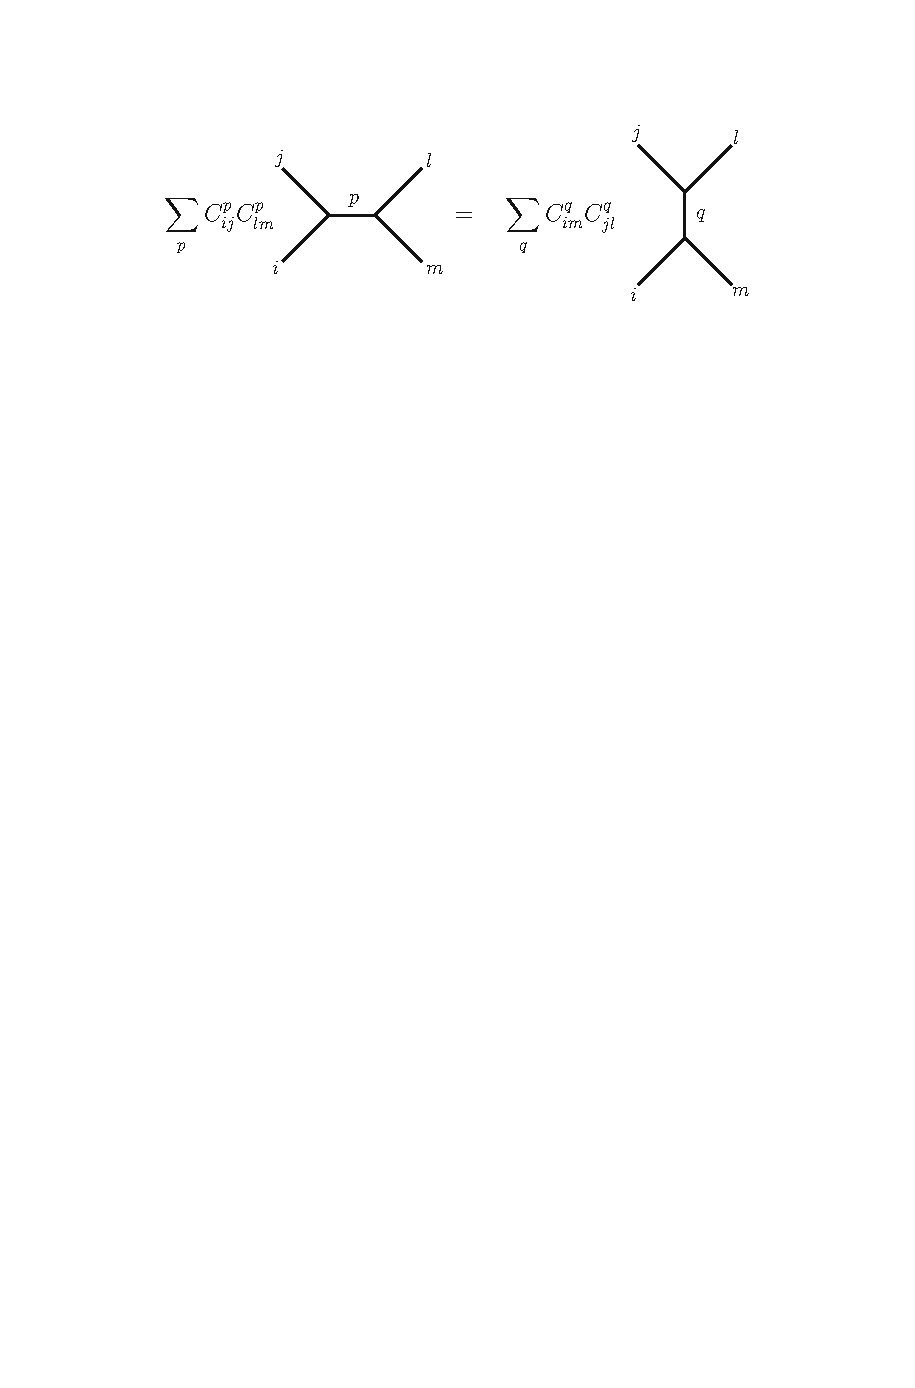
\includegraphics{figs/fig10.pdf}
	\caption{$G(x)=G(1-x)$ Crossing Symmetry的图示}
\end{figure}
\subsection{Fusing and Braiding Matrices}
考虑一个比较简单的情形,CFT的谱是个有限谱\sn{比如RCFT},这样Conformal Blocks构成了一个有限维线性空间,其中的某个线性组合得到的元素就是我们要的四点关联函数\sn{当然还要把全纯反全纯组合起来}。这其实就是在说\ref{32.3},\ref{32.6}和\ref{32.7}中的Conformal Blocks相差的仅仅是一个线性变换,他们是同一个线性空间的不同基底!
\begin{equation}
	\mathcal{F}_{ij}^{kl}(p\mid x)=\sum_qB{\left[\begin{smallmatrix}j&k\\i&l\end{smallmatrix}\right]}_{p,q}\mathcal{F}_{ik}^{jl}\!\left(q\mid\frac1x\right)
\end{equation}
\begin{equation}
	\mathcal{F}_{ij}^{kl}(p\mid x)=\sum_qF{\left[\begin{array}{cc}j&k\\i&l\end{array}\right]}_{p,q}\mathcal{F}_{il}^{jk}(q\mid1-x)
\end{equation}
这里$B$称作\textbf{Braiding Matrices},$F$称作\textbf{Fusing Materices},$p,q$是标记矩阵元,$\{i,j,l,m\}$标记矩阵本身。我们用类似轮换序图的形式来表达上面的两个方程:
\begin{figure}[H]
	\centering
	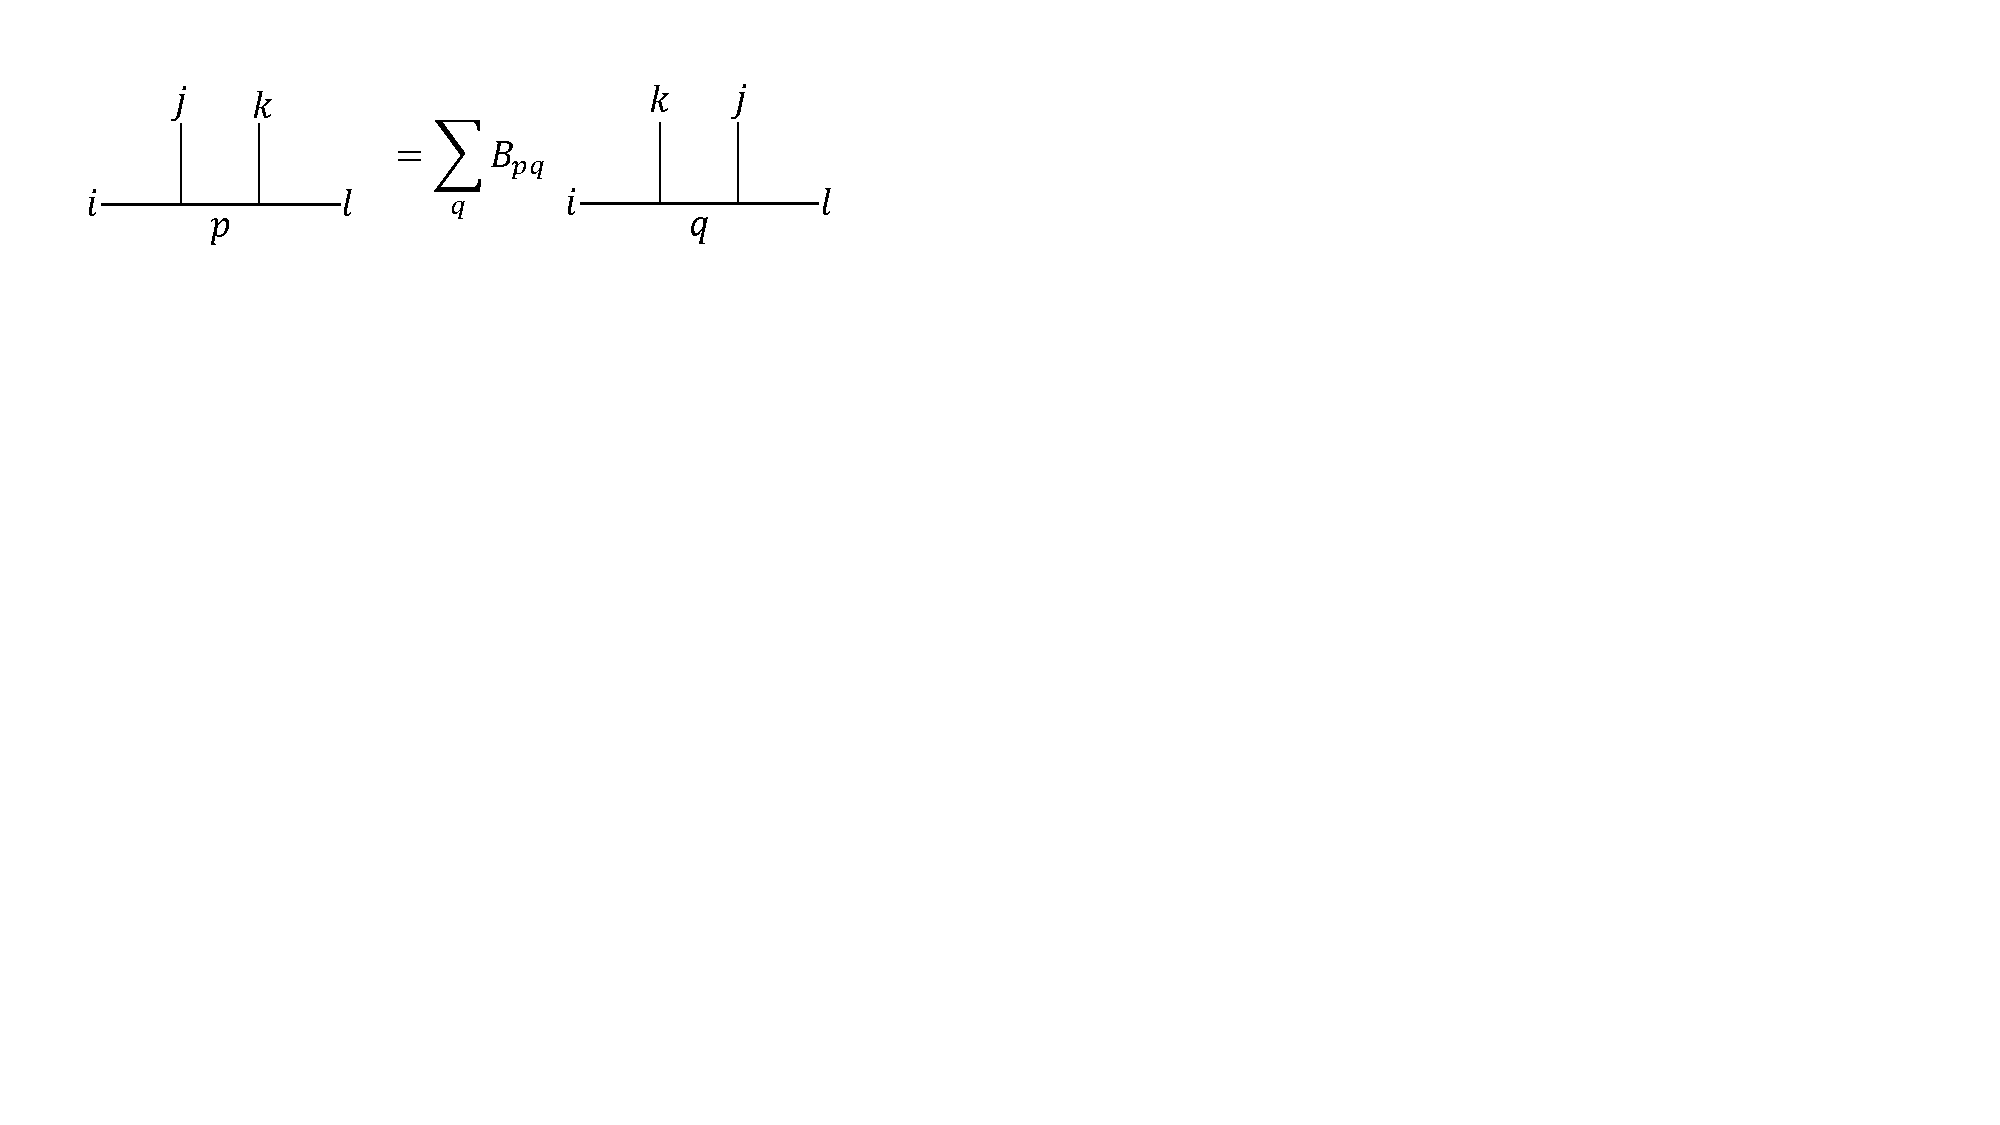
\includegraphics[width=0.8\linewidth]{figs/fig11.pdf}
\end{figure}
\begin{figure}[H]
	\centering
	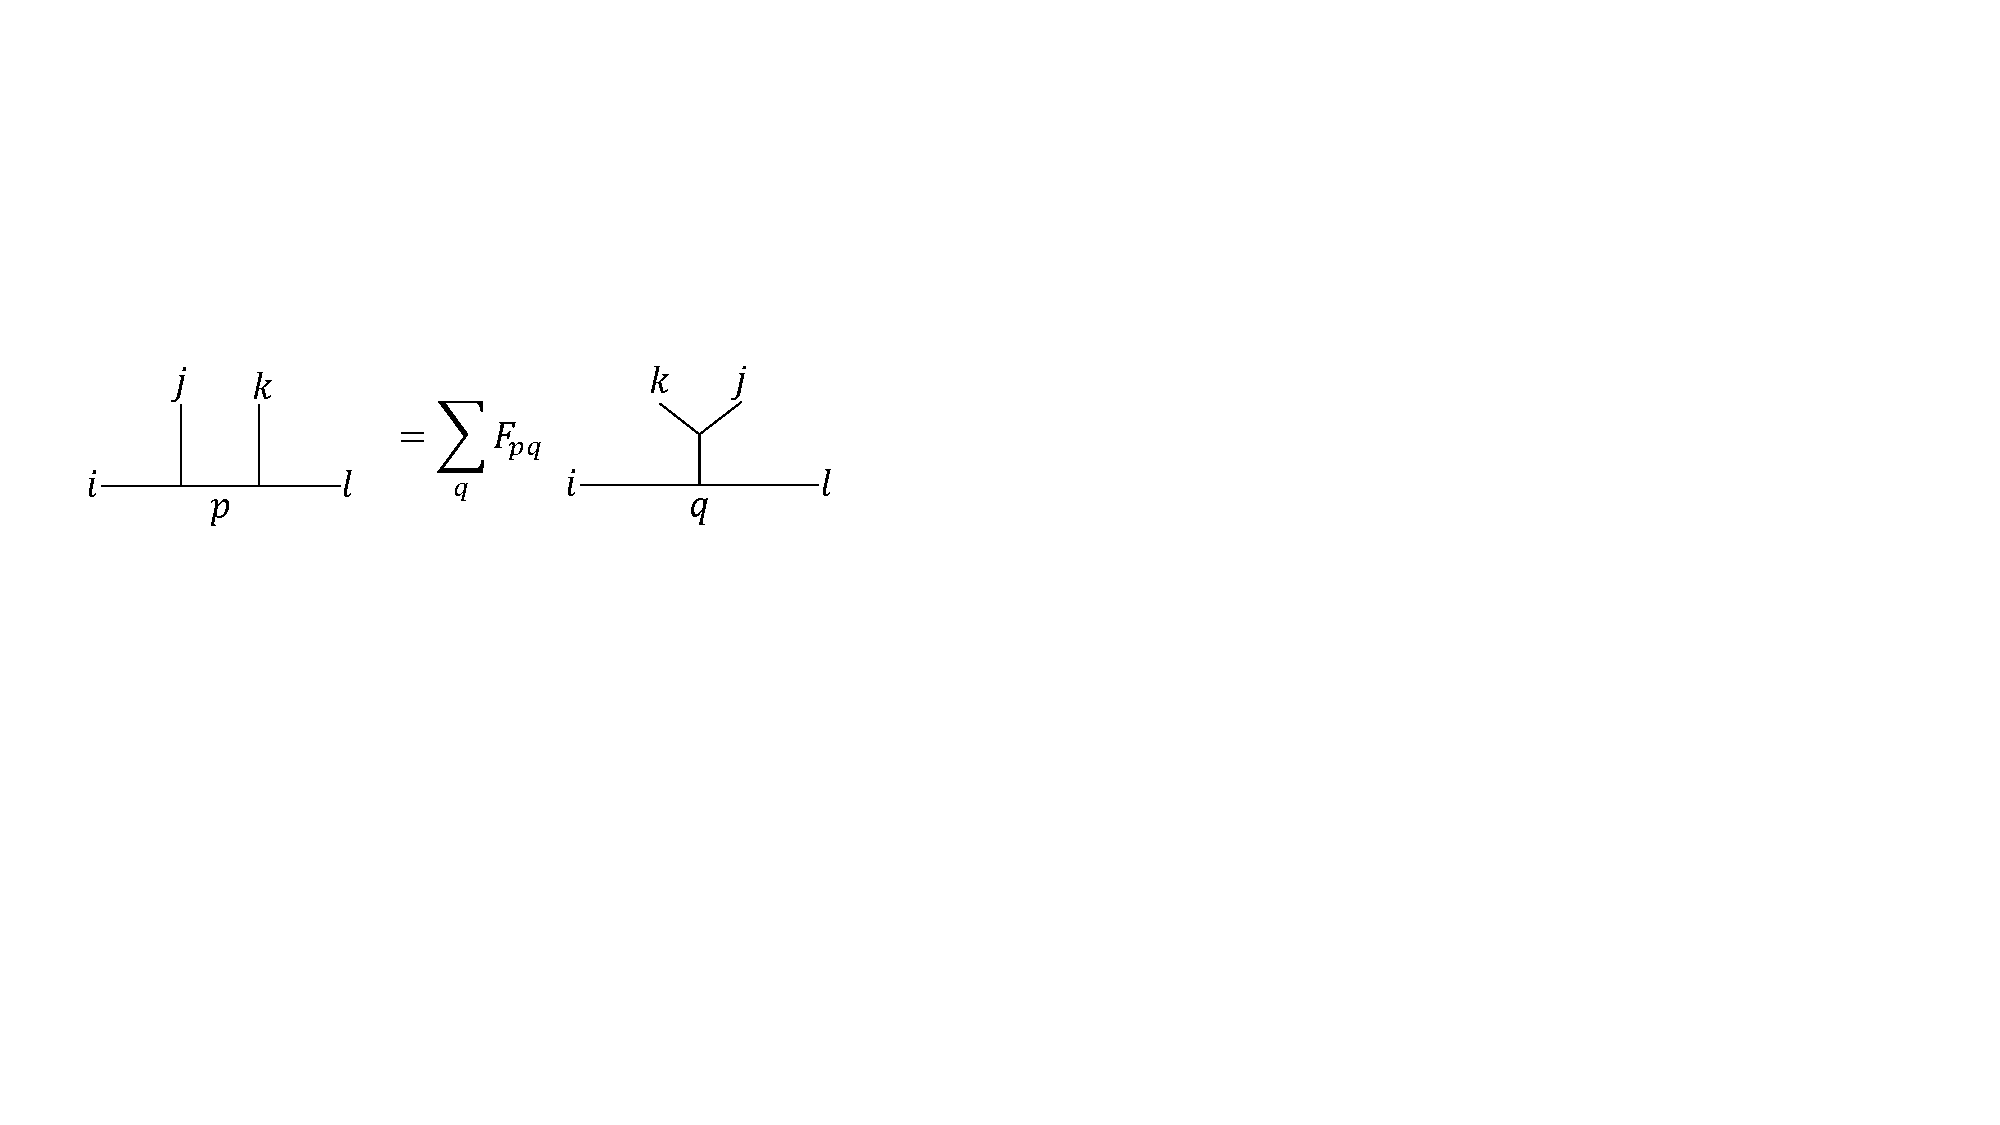
\includegraphics[width=0.8\linewidth]{figs/fig12.pdf}
\end{figure}
利用下面图表的交换性:
\begin{figure}[H]
	\centering
	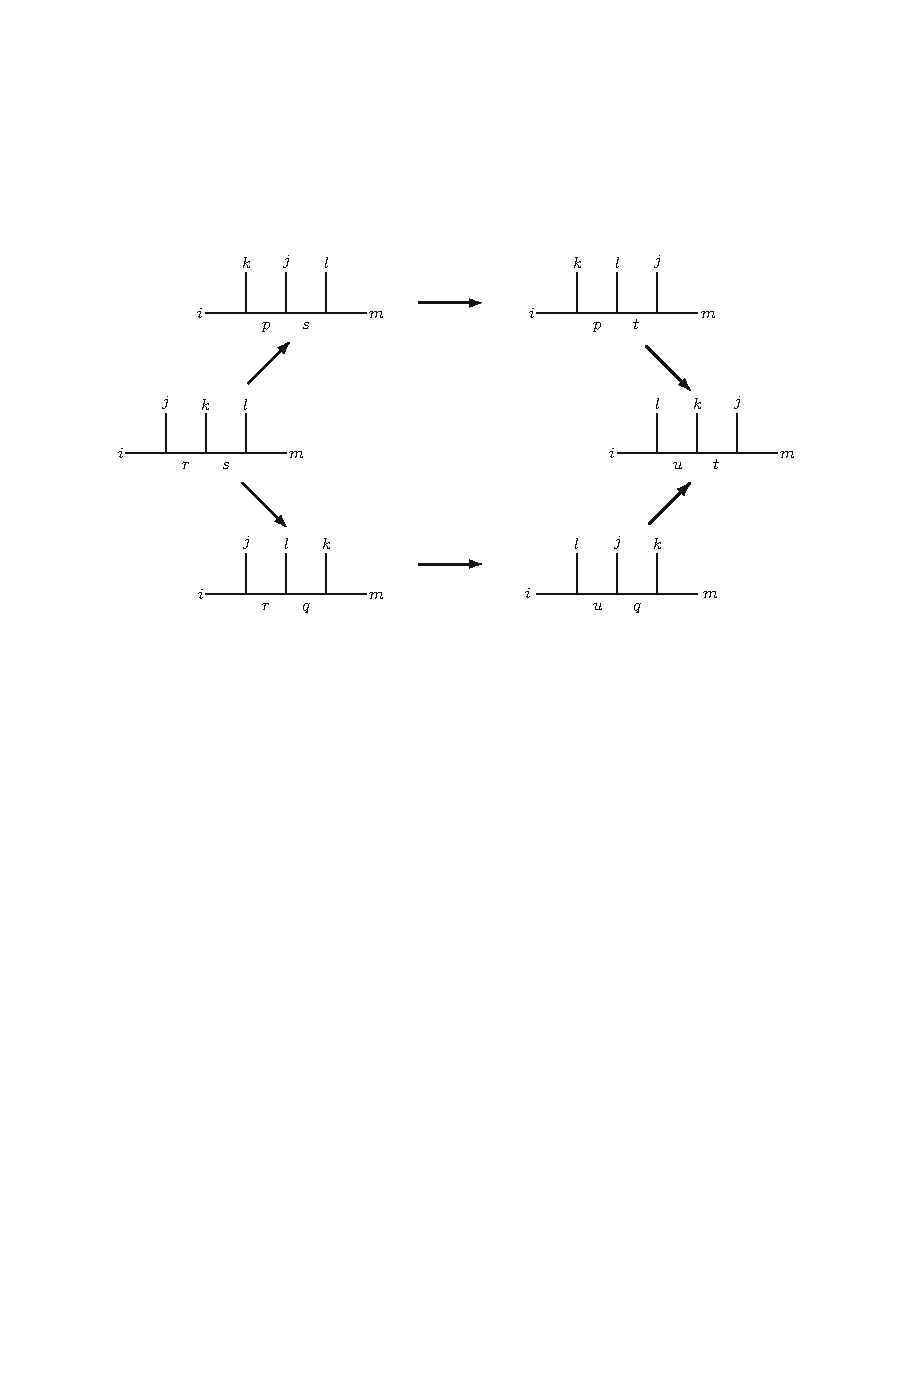
\includegraphics{figs/fig13.pdf}
\end{figure}
得到hexgon恒等式:
\begin{equation}
	\boxed{
		\sum_{p} B\left[\begin{array}{cc}
			j & k \\
			i & s
		\end{array}\right]_{r p} B\left[\begin{array}{cc}
			j & l \\
			p & m
		\end{array}\right]_{s t} B\left[\begin{array}{cc}
			k & l \\
			i & t
		\end{array}\right]_{p u}=\sum_{q} B\left[\begin{array}{cc}
			k & l \\
			r & m
		\end{array}\right]_{s q} B\left[\begin{array}{cc}
			j & l \\
			i & q
		\end{array}\right]_{r u} B\left[\begin{array}{cc}
			j & k \\
			u & m
		\end{array}\right]_{q t}
	}
\end{equation}
上面的方程非常像Yang-Baxter方程,所以CFT和可积性有很大的关联。但是注意上面这不是证明!就和YBE的图形化规则推导一样,只是便于计算和记忆。同样根据下面的图表交换:
\begin{figure}[H]
	\centering
	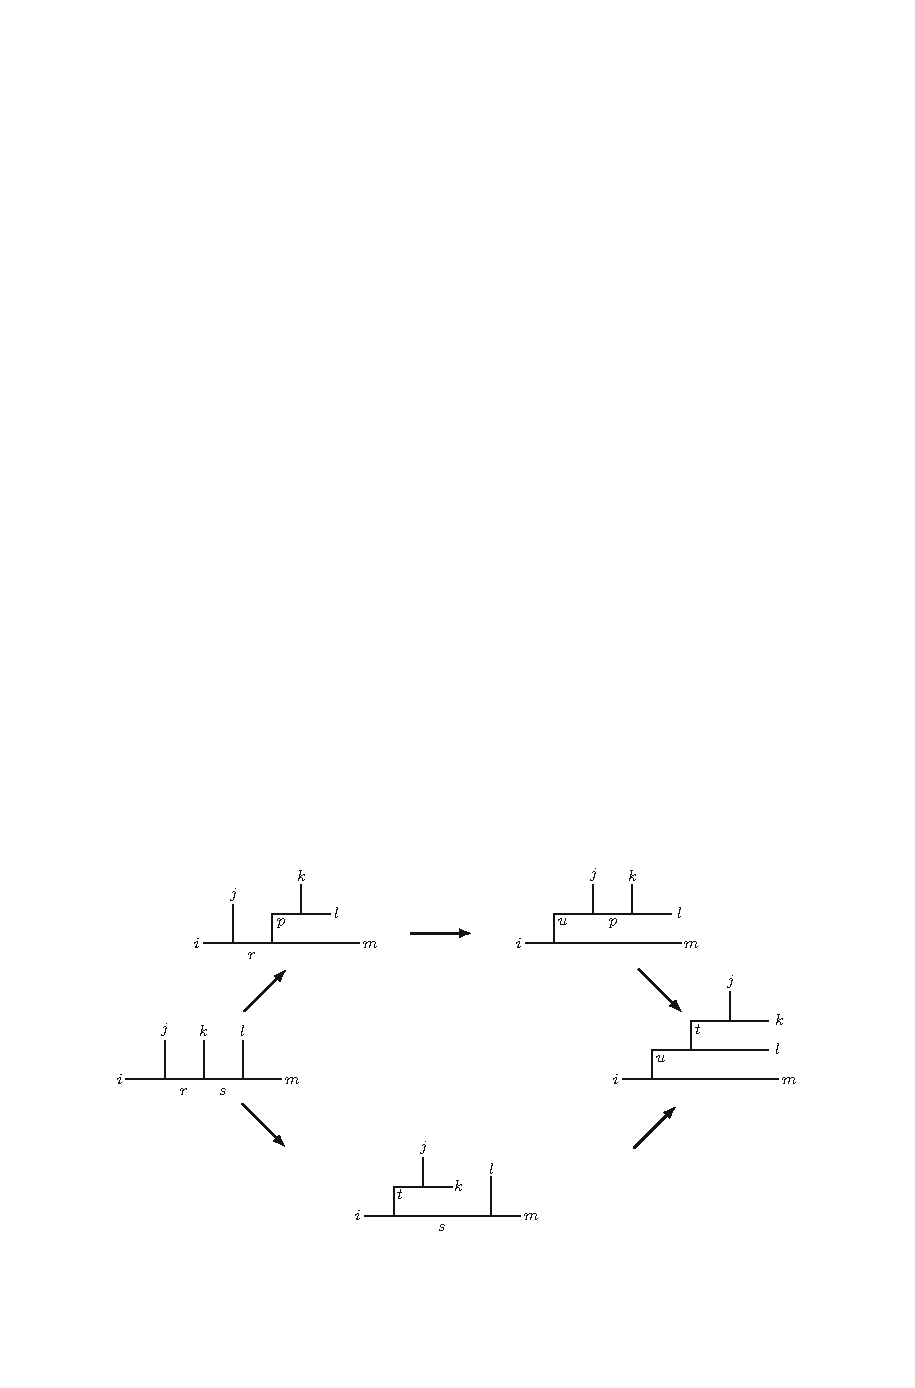
\includegraphics{figs/fig14.pdf}
\end{figure}
得到pentagon恒等式:
\begin{equation}
	\boxed{
		 F\left[\begin{array}{cc}
			j & k \\
			i & s
		\end{array}\right]_{r t} F\left[\begin{array}{cc}
			t & l \\
			i & m
		\end{array}\right]_{s u} =\sum_{p} F\left[\begin{array}{cc}
			k & l \\
			r & m
		\end{array}\right]_{s p} F\left[\begin{array}{cc}
			j & p \\
			i & m
		\end{array}\right]_{r u} F\left[\begin{array}{cc}
			j & k \\
			u & l
		\end{array}\right]_{p t}
	}
\end{equation}
\section{NOPs and Conformal family}
\subsection{Normal Ordered Products}
两个算符的OPE在两个算符的插入位置一样时会发散,这种发散就类似于一般QFT中的红外发散,因为空间无限大,所以真空零点能发撒,这种发散可以通过取算符的正规乘积(NOP)得到,共形场论也有这样的做法。我们先考虑\textbf{自由场},也就是$R(\phi\partial^n\phi)$最多只有一项是奇异的,\sn{对到QFT那边就是场的模式展开可以完全分离成产生算符和湮灭算符之和}那么我们直接减去真空期望值就去除了所有的发散项,所以NOP可以定义为:
\begin{definition}[NOPs]
	\begin{equation}
		:\phi_1(z)\phi_2(w):\equiv\left(\phi_1(z)\phi_2(w)-\left\langle{\phi_1(z)\phi_2(w)}\right\rangle\right):
	\end{equation}
	这里省略了所有的径向排序,记收缩:
	\begin{equation}
		\wick{\c \phi(z)\c \phi(w)}\equiv \left\langle{\phi_1(z)\phi_2(w)}\right\rangle
	\end{equation}
	缩并后是一个数,可以提出去。显然在$z\to w$后OPE的所有奇异性都被减除:
	\begin{equation}
		:\phi_1\phi_2:(w)\equiv\lim_{z\to w}\left(:\phi_1(z)\phi_2(w):\right)
	\end{equation}
\end{definition}
\begin{theorem}[Wick]
	\begin{equation}
		\boxed{
			\begin{aligned}
				\mathsf R[\Phi_{a_1}(x_1)\Phi_{a_2}(x_2)\cdots\Phi_{a_n}(x_n)]=\mathsf N\big[&\Phi_{a_1}(x_1)\Phi_{a_2}(x_2)\cdots\Phi_{a_n}(x_n)\\&+\left(\Phi_{a_1}\Phi_{a_2}\cdots\Phi_{a_n}\text{的所有可能缩并}\right)\big]
			\end{aligned}
		}
	\end{equation}
	由于正规序插入到真空态之间恒为0,所以任何没有完全缩并的项对真空期望值都没有贡献。
\end{theorem}
\begin{proof}
	关于Wick定理的证明可见任何一本正则量子化的QFT教材,比如余钊焕老师的讲义\footnote{\url{http://yzhxxzxy.github.io/cn/teaching.html}},这里只想强调定理本身依赖于前面对自由场的NOP定义。
\end{proof}
\begin{example}
	\begin{equation}
		\begin{aligned}\mathsf{R}(\Phi_a\Phi_b\Phi_c\Phi_d)&=\mathsf{N}\big(\Phi_a\Phi_b\Phi_c\Phi_d+\wick{\c \Phi_a\c\Phi_b\Phi_c\Phi_d}+\wick{\c\Phi_a\Phi_b\c\Phi_c\Phi_d}+\wick{\c\Phi_a\Phi_b\Phi_c\c\Phi_d}\\&\quad\quad+\wick{\Phi_a\c\Phi_b\c\Phi_c\Phi_d}+\wick{\Phi_a\c\Phi_b\Phi_c\c\Phi_d}+\wick{\Phi_a\Phi_b\c\Phi_c\c\Phi_d}\\&\quad\quad+\wick{\c\Phi_a\c\Phi_b}\wick{\c\Phi_c\c\Phi_d}+\wick{\c1\Phi_a\c2\Phi_b\c1\Phi_c\c2\Phi_d}+\wick{\c1\Phi_a\c2\Phi_b\c2\Phi_c\c1\Phi_d}\big)\end{aligned}
	\end{equation}
	计算的下一步是将所有收缩的项放在一起,未收缩的项放在一起,对于玻色场由于满足对易关系可以随便移动场的位置,这一步是trivial的,不过费米场因为满足反对易关系,所以交换两个场位置时会产生一个负号需要额外注意。
	
	左边减去右边,并取$x_a,x_b\to x$和$x_c,x_d\to y$的极限后得到两个NOP的时序积的Wick定理:
	\begin{equation}\label{33.6}
		\begin{aligned}
			\mathsf{R}\left[:\Phi_a\Phi_b:(x):\Phi_c\Phi_d:(y)\right]&=\mathsf{N}\big(\Phi_a\Phi_b\Phi_c\Phi_d+\wick{\c\Phi_a\Phi_b\c\Phi_c\Phi_d}+\wick{\c\Phi_a\Phi_b\Phi_c\c\Phi_d}\\&\quad\quad+\wick{\Phi_a\c\Phi_b\c\Phi_c\Phi_d}+\wick{\Phi_a\c\Phi_b\Phi_c\c\Phi_d}\\&\quad\quad+\wick{\c1\Phi_a\c2\Phi_b\c1\Phi_c\c2\Phi_d}+\wick{\c1\Phi_a\c2\Phi_b\c2\Phi_c\c1\Phi_d}\big)
		\end{aligned}
	\end{equation}
	这个计算实际上是非常一般的,他告诉我们计算NOP的时序积时跟没有NOP时一样计算,但是认为NOP内部的场之间的收缩为0。
\end{example}
\begin{remark}
	下面是一些比较有用的缩并等式:
	\begin{equation}
		\wick{\c A(z)\c{:B^{n}:}}(w)=n\wick{\c A(z)\c B(w)}:B^{n-1}(w):
	\end{equation}
	\begin{equation}
		\wick{\c A(z):\c {e}^{B(w)}:}=\wick{\c A(z)\c B(w)}:e^{B(w)}:
	\end{equation}
	\begin{equation}\label{33.9}
		\begin{aligned}
			\wick{:\c{e}^{A(z)}::\c{e}^{B(z)}:}&=\sum_{m,n,k}\frac{k!}{m!n!}\begin{pmatrix}m\\k\end{pmatrix}\begin{pmatrix}n\\k\end{pmatrix}[\wick {\c A(z)\c B(w)}]^k:A^{m-k}(w)B^{n-k}(w):\\&=\exp\left\{\wick{\c A(z)\c B(w)}\right\}:e^{A(w)}e^{B(w)}:\end{aligned}
	\end{equation}
\end{remark}
但是对于非自由场,NOP不能这么定义,比如$TT$的NOP照此定义,仍然发散,所以对于一般场的NOP应当定义成减去所有的奇异项。
\begin{definition}
	\begin{equation}
		\left(A(z)B(w)\right)\equiv A(z)B(w)-\wick{\c A(z)\c B(w)}
	\end{equation}
	这里$\wick{\c A(z)\c B(w)}$表示OPE的\textbf{所有}奇异部分。注意我们引入了文献中另外一种表示NOP的方式:$\left(\cdot\right)$。同样,定义:
	\begin{equation}
		\left(AB\right)(w)=\lim_{z\to w} \left(A(z)B(w)\right)
	\end{equation}
\end{definition}
将NOP其中一个场做洛朗展开,然后可以将OPE用NOP表达为:
\begin{theorem}[NOPs $\iff$ OPEs]
	\begin{equation}
		\phi(z)\chi(w)=\operatorname{sing.}+\sum_{n=0}^\infty\frac{(z-w)^n}{n!}N\big(\partial^n\phi\chi\big)(w)
	\end{equation}
	同样可以用OPE表达NOP:
	\begin{equation}
		N\left(\phi\chi\right)(w)=\oint_{\mathcal{C}(w)}\frac{dz}{2\pi i}\frac{\phi(z)\chi(w)}{z-w}
	\end{equation}
\end{theorem}
考虑NOP的Laurent模:
\begin{equation}
	\begin{aligned}N\left(\phi\chi\right)&(w)=\sum_{n\in\mathbb{Z}}w^{-n-h^\phi-h^\chi}N\left(\phi\chi\right)_n,\\N\left(\phi\chi\right)_n&=\oint_{\mathcal{C}(0)}\frac{dw}{2\pi i}w^{n+h^\phi+h^\chi-1}N\left(\phi\chi\right)(w)\end{aligned}
\end{equation}
\begin{theorem}
	\begin{equation}
		\boxed{
		N\left(\phi\chi\right)_{n}=\sum_{k>-h^{\phi}}\chi_{n-k}\phi_{k}+\sum_{k\leq-h^{\phi}}\phi_{k}\chi_{n-k}
		}
	\end{equation}
\end{theorem}
\begin{proof}
	\begin{equation}
		\begin{aligned}N\left(\phi\chi\right)_n&=\oint_{C(0)}\frac{dw}{2\pi i}w^{n+h^\phi+h^{\lambda}-1}\oint_{C(w)}\frac{dz}{2\pi i}\frac{\phi(z)\chi(w)}{z-w}\\&=\underbrace{\oint\frac{dw}{2\pi i}w^{n+h^\phi+h^{\lambda}-1}\Big(\underbrace{\oint_{|z|>|w|}\frac{dz}{2\pi i}\frac{\phi(z)\chi(w)}{z-w}}_{\mathcal{I}_1}}_{\mathcal{I}_2}-\oint_{|z|<|w|}\frac{dz}{2\pi i}\frac{\chi(w)\phi(z)}{z-w}\Big)\end{aligned}
	\end{equation}
	计算$\mathcal{I}_1$得到:
	\begin{equation}
		\begin{aligned}
			\mathcal{I}_{1}& =\oint_{|z|>|w|}\frac{dz}{2\pi i}\frac{1}{z-w}\sum_{r,s}z^{-r-h^{\phi}}w^{-s-h^{\chi}}\phi_{r}\chi_{s}  \\
			&=\oint_{|z|>|w|}\frac{dz}{2\pi i}\left.\frac1z\sum_{p\geq0}\left(\frac wz\right)^p\sum_{r,s}z^{-r-h^\phi}w^{-s-h^\chi}\phi_r\chi_s\right.  \\
			&=\oint_{|z|>|w|}\frac{dz}{2\pi i}\sum_{p\geq0}\sum_{r,s}z^{-r-h^\phi-p-1}w^{-s-h^\chi+p}\phi_r\chi_s.
		\end{aligned}
	\end{equation}
	频繁利用Cauchy积分公式得到:
	\begin{equation}
		\begin{aligned}
			\mathcal{I}_2&=\oint\frac{dw}{2\pi i}\sum_{p\geq0}\sum_sw^{-s-h^x+p+n+h^\phi+h^x-1}\phi_{-h^\phi-p}\chi_s\\
			&=\sum_{p\geq0}\phi_{-h^\phi-p}\chi_{h^\phi+n+p}=\sum_{k\leq-h^\phi}\phi_k\chi_{n-k}
		\end{aligned}
	\end{equation}
	对另外一项也同样计算就可以证明这个及其重要的等式了。
\end{proof}
这个等式其实非常好理解,从前面对CFT的希尔伯特空间构造可以看到,一个场的Laurent模当$n>-h$时是湮灭算符,$n\leq-h$时是产生算符,所以这个等式的含义就是相对$\phi$而言将所有的产生算符排在前面,湮灭算符放在后面,这正是在QFT中对NOP最naive的定义!

另外,NOP与OPE最大的不同是他并不满足交换律和结合律,这也意味着对多个算符的NOP定义有歧义\sn{对于自由场,前面的定义还是well-define的},往往选取的是下面的嵌套定义:
\begin{equation}
	(ABC\cdots DE)\equiv(A(B(C(\cdots(DE))))))
\end{equation}
另外,Wick定理也失效了,不过我们有下面的等式:
\begin{theorem}[Generalized Wick]
	\begin{equation}\label{wick}
		\boxed{
			{A(z)(BC)}(w)=\frac1{2\pi i}\oint_{\mathcal{C}(w)}\frac{dx}{x-w}\left\{\wick{\c A(z)\c B}(x)C(w)+B(x)\wick{\c A(z)\c C}(w)\right\}+\text{regular}
		}
	\end{equation}
\end{theorem}
上式是对自由场的下面特殊的Wick定理的相互作用推广:
\begin{equation}
	\phi_1(x):\phi_2\phi_3:(y)=\wick{\c\phi_1(x)\c\phi_2(y)}:\phi_3(y):+\wick{\c\phi_1(x)\c\phi_3(y)}:\phi_2(y):+\underbrace{:\phi_1(x)\phi_2(y)\phi_3(y):}_{\text{regular}}
\end{equation}
还可以证明,虽然结合律失效了,但是有下面等式:
\begin{theorem}[Rearrangement Lemma]
	\begin{equation}
		((AB)E)-(A(BE))=(A([E,B]))+(([E,A])B)+([(AB),E])
	\end{equation}
	$E$一般取为$(CD)$。
\end{theorem}
$T$不是初级场,$N(TT)$也不是初级场,但是下面定义的$\mathcal{N}(TT)$是共形权为$(4,0)$的初级场:
\begin{equation}\label{33.23}
	\boxed{
		\mathcal{N}(TT)=N\left(TT\right)-\frac3{10}\partial^2T
	}
\end{equation}
后面会用到这个式子。
\subsection{Verma module}
从真空态出发,将$L_n$作为产生算符作用上去,得到的一系列态成为Verma模:
\begin{definition}[Verma Module]
	\begin{equation}
		\boxed{
			\left\{L_{k_1}\ldots L_{k_n}|0\rangle|k_i\leq-2\right\}
		}
	\end{equation}
	中的元素称为Verma Module。
\end{definition}
根据态算符对应,每一个Verma Module都会对应一个场(不一定是初级场),可以证明这些场一定是能动张量或者其偏导或者它们的NOP:
\begin{equation}
	\boxed{
		F\in\left\{T,\partial T,\ldots,N(\ldots)\right\}
	}
\end{equation}
\subsection{Descendant states}
前面是考虑一个真空态开始往上构造其它态,由于:
\begin{equation}
	L_n\left|\phi\right\rangle=\left[L_n,\phi_{-h}\right]\left|0\right\rangle=\left(h\left(n+1\right)-n\right)\phi_{-h+n}\left|0\right\rangle=0,\quad n>0
\end{equation}
所以初级场作用在真空态上构造的$\ket{\phi}$也比较特殊,和真空态一样被所有的$L_n$湮灭算符湮灭,所以也可以考虑从$\ket{\phi}$开始构造其它态:
\begin{definition}[Descendant States]
	\begin{equation}
		\boxed{
			\left\{L_{k_1}\ldots L_{k_n}|\phi\rangle:\mathrm{~}k_i\leq-1\right\}
		}
	\end{equation}
	其中$\phi$是任意一个初级场。这些态称为初级场的次级态(descendant states)。
\end{definition}
\begin{table}[H]
\centering
\begin{tabular}{lrc}
	\text { Field } & \text { State } & \text { Level } \\
	\hline \hline$ \phi(z)$& $\phi_{-h}|0\rangle=|h\rangle$ & $0 $\\
	\hline $\partial \phi $& $L_{-1} \phi_{-h}|0\rangle $& $1$ \\
	\hline$ \partial^{2} \phi $& $L_{-1} L_{-1} \phi_{-h}|0\rangle $& $2 $\\
	$N(T \phi)$ &$ L_{-2} \phi_{-h}|0\rangle$ & 2 \\
	\hline $\partial^{3} \phi$ & $L_{-1} L_{-1} L_{-1} \phi_{-h}|0\rangle$ & $3$ \\
	$N(T \partial \phi)$ &$ L_{-2} L_{-1} \phi_{-h}|0\rangle $&$ 3$ \\
	$N(\partial T \phi) $& $L_{-3} \phi_{-h}|0\rangle $& $3$ \\
	\hline \ldots & \ldots & \ldots
\end{tabular}
\caption{次级态和次级场之间的对应}
\label{descendant}
\end{table}
同样根据态算符对应,这些态也会对应到一些场,根据上面的表就可以猜到是:
\begin{equation}
	\boxed{
		\left[\phi(z)\right]:=\left\{\phi,\partial\phi,\partial^2\phi,\ldots,N(T\phi),\ldots\right\}
	}
\end{equation}
我们成为$\phi$的Conformal Family。Verma Module是直接真空态生成来的,真空态对应$h=0$,可以用$[1]$来标记这个特殊的Conformal Family。

注意到在上面的表中我们写下来对应的Level,注意到$L_0$可看作体系的哈密顿量,真空态对应能量0,初级场$\ket{h}$对应能量$h$,而作用$L_{-k}$上去会把能量加$k$,所以这就跟量子力学中谐振子问题作用产生算符得到更高能级的态一样。只不过这里能级都是简并的,而简并态数目的计数在后面的环面CFT配分函数构造上有很大的作用,对于Verma module(真空态毕竟唯一),或者$\ket{h}$本身不简并的Conformal Family来说,设$P(N)$是第$N$个Level简并度,则其有下面的生成函数:
\begin{equation}
	\boxed{
		\prod_{n=1}^\infty\frac1{1-q^n}=\sum_{N=0}^\infty P(N)q^N
	}
\end{equation}

次级态和次级场之间用NOP对应,而NOP天然的和OPE有对应,所以实际上我们可以用OPE的围道积分来表示:
\begin{theorem}
	用$\widehat{L}_{-n}\phi(w)$表示$L_{-n}\ket\phi$对应的次级场,那么:
	\begin{equation}\label{eq:33.30}
		\boxed{
			\widehat{L}_{-n}\phi(w)=\oint_{\mathcal{C}(w)}\frac{dz}{2\pi i}\frac1{(z-w)^{n-1}}T(z)\phi(w)
		}
	\end{equation}
\end{theorem}
\begin{proof}
	利用态算符对应,取$w\to 0$的极限就能看出正确性了。代入OPE实际计算几个例子也能得到表\ref{descendant}的结果。
\end{proof}
现在我们来证明CFT自举里面非常重要的一个微分方程,核心目的是将次级态和其他初级场的关联函数用其他初级场的关联函数来表示。
\begin{theorem}
	$\phi,\phi_1,\ldots,\phi_N$是初级场,则:
	\begin{equation}\label{33.31}
		\boxed{
			\begin{gathered}
				\left\langle\widehat{L}_{-n}\phi(w)\phi_{1}(w_{1})\ldots\phi_{N}(w_{N})\right\rangle=\mathcal{L}_{-n}\langle\phi(w)\phi_{1}(w_{1})\ldots\phi_{N}(w_{N})\rangle  \\
				\text{Where,}\qquad\mathcal{L}_{-n}=\sum_{i=1}^N\left(\frac{(n-1)h_i}{(w_i-w)^n}-\frac1{(w_i-w)^{n-1}}\partial_{w_i}\right)
			\end{gathered}
		}
	\end{equation}
\end{theorem}
\begin{proof}
	\begin{equation}
		\begin{aligned}
			&\left\langle\widehat{L}_{-n}\phi(w)\phi_1(w_1)\ldots\phi_N(w_N)\right\rangle  \\
			=&\oint_{\mathcal{C}(w)}\frac{dz}{2\pi i}\left.(z-w)^{1-n}\left\langle\left(T(z)\phi(w)\right)\phi_1(w_1)\ldots\phi_N(w_N)\right\rangle\right.  \\
			=&-\sum_{i=1}^N\oint_{\mathcal{C}(w_i)}\frac{dz}{2\pi i}\left.(z-w)^{1-n}\left\langle\phi(w)\phi_1(w_1)\ldots\left(T(z)\phi_i(w_i)\right)\ldots\phi_N(w_N)\right\rangle\right.  \\
			=&-\sum_{i=1}^N\oint_{\mathcal{C}(w_i)}\frac{dz}{2\pi i}\left(z-w\right)^{1-n}\times  \\
			&\times\left(\frac{h_i}{(z-w_i)^2}+\frac1{z-w_i}\partial_{w_i}\right)\left\langle\phi(w)\phi_1(w_1)\ldots\phi_N(w_N)\right\rangle  \\
			=&-\sum_{i=1}^N\left((1-n)\left(w_i-w\right)^{-n}h_i+\left(w_i-w\right)^{1-n}\partial_{w_i}\right)\left<\phi(w)\phi_1(w_1)\ldots\phi_N(w_N)\right>
		\end{aligned}
	\end{equation}
	上面证明中第二个等号利用了全平面内极点留数只和为0,第三个等号利用了初级场OPE。
\end{proof}
\section{Representations of the Virasoro Algebra}
现在来从群表示的观点看下我们前面的Verma Module和Conformal Family实在做什么。前面反复强调如果我们有了一个理论的对称代数,那么确定其希尔伯特空间就是在找群表示。最简单的CFT就是只有Virasoro代数作为其对称代数,由于这时左右模完全分离,所以我们可以先分开讨论,然后$\bigoplus_{\{h,\bar h\}} V_{c,h}\otimes V_{c,\bar h}$就构成了整个表示空间\sn{也正因为完全分离,这里$h,\bar h$直积时无特殊要求,后面玻色子我们会看到一个有要求的最简单的例子。}。

我们要找的表示是所谓最高权表示,从量子力学的角度去想,构造谱的第一步是去找CSCO,由于理论没有其他对称性,也就是说没有其他力学量和$L_0$对易,所以我们期望构造的谱是$L_0$的本征值。进一步,由于$\{L_n,n\geq0\}$构成了理论的湮灭算符,所以我们先找到被所有湮灭算符湮灭的那些态:
\begin{equation}
	\begin{aligned}L_n\left|h\right\rangle&=0\quad\text{for}\quad n>0,\\L_0\left|h\right\rangle&=h\left|h\right\rangle\end{aligned}
\end{equation}
找到了所有的最高权之后,下一步就是将产生算符$\{L_{n},n<0\}$作用到上面构造能量更高的态:\sn{这些态都是$L_0$的本征态,但是我们并不用$\ket{h+k}$这样的记号标记他们,因为要和最高权区分。}
\begin{equation}
	L_{-1}\ket{h},\quad L_{-2}\ket{h},\quad L_{-1}L_{-1}\ket{h},\quad L_{-3}\ket{h},\quad\ldots
\end{equation}
不难发现,最高权就是真空态和理论中的初级态,而其他用产生算符构造的态就是Verma module和descendant states。

但是这只是从数学上构造出了这些态,真正物理的态最大的特点就是可归一化,所以那些模方为0的态要被剔除出去,比如说前面在构造Verma Module时,就没有把$L_{-1}\ket{0}$算进去,后面我们会进一步阐明如何找到其它的模方为0的态。进一步如果要求理论是幺正的,那些模方为负数的表示还要整个剔除掉。\sn{注意,幺正性要求那些有模方为负数的次级态的表示是被禁闭的,而不是像模方为0的态稍微剔除一下就好。}

如果理论还存在更大的对称性,这个时候CSCO就会加入其他的和${L_0}$对易的算符,谱将会同时对角化CSCO中的算符,即最高权现在由更多量子数标记$\ket{h,q}$。而且产生湮灭算符也不只有$\{L_{n},n<0\}$了,构造次级态还需要用理论中其他的产生湮灭算符去作用。这在数学上本身就是个非常麻烦的事情,后面我们并不追求数学上的一般性和严谨性,只是给些例子。

\section{Free CFT}
学习CFT最好的方式是给出一些具体的例子,首先我们考虑最简单的自由CFT。
\subsection{Free Bosons}
自由玻色场可以从圆柱上定义的标量场量子化后得来,这里直接给出二维CFT的版本\sn{已经做了Wick转动,$\kappa$是弦论来的耦合常数}:
\begin{equation}
	\begin{aligned}
		\text{S}& =\frac1{4\pi\kappa}\int dzd\overline{z}\sqrt{|g|}g^{ab}\partial_aX\partial_bX  \\
		&\xleftarrow{\kappa=1}\frac1{4\pi}\int dzd\overline{z}\partial X\cdot\overline{\partial}X
	\end{aligned}
\end{equation}
其中度规是从圆柱上的平直度规转到复平面上的度规:
\begin{equation}
	\left.g_{ab}=\left[\begin{array}{cc}0&\frac{1}{2z\overline{z}}\\\frac{1}{2z\overline{z}}&0\end{array}\right.\right],\quad g^{ab}=\left[\begin{array}{cc}0&2z\overline{z}\\2z\overline{z}&0\end{array}\right]
\end{equation}
再次强调CFT的定义根本不需要拉氏量,这里只是更场论一点的出发方式。直接读出运动方程:\sn{这也说明$X(z,\bar z)$总是可以写成全纯和反全纯部分之和}
\begin{equation}
	\partial\overline{\partial}X(z,\overline{z})=0
\end{equation}
可以定义下面两个手征场:
\begin{equation}\label{35.4}
	j(z)=i\partial X(z,\overline z),\quad\bar j(\overline z)=i\overline\partial X(z,\overline z)
\end{equation}
还可以读出传播子$K\equiv\left\langle{X(z,\bar z)X(w,\bar w)}\right\rangle$:
\begin{equation}
	\partial_z\partial_{\overline{z}}K(z,\overline{z},w,\overline{w})=-2\pi\delta^{(2)}(z,-w)\Rightarrow K=-\log\left|z-w\right|^2
\end{equation}
这直接说明了$X$不是初级场,但是:
\begin{equation}
	\left\langle j(z)j(w)\right\rangle=\frac{1}{(z-w)^2}
\end{equation}
说明了$j(z)$是$h=1$的初级场,也得到了OPE:\sn{由于OPE的最奇异项只能是二次的,而一次的又破坏了$z\leftrightarrow w$的对称性。}
\begin{equation}\label{35.7}
	\boxed{
		j(z)j(w)=\partial_z X(z)\partial_w X(w)=\frac{1}{(z-w)^2}+\ldots
	}
\end{equation}
根据OPE很容易算出对易关系:
\begin{equation}
	\boxed{
		\begin{bmatrix}j_m,j_n\end{bmatrix}= m\delta_{m+n,0}
	}
\end{equation}
根据$j$是共形权为1的初级场很容易证明作用量的确是共形不变的\sn{不少文献数量纲之后根据尺度不变性直接说明共形不变,绝大多数情况下这没问题,甚至一度让人们觉得尺度不变蕴含共形不变。但是上世纪八十年代Polchinski就研究了反例\cite{Polchinski:1987dy}}。下面演示如何通过作用量确定CFT中最关键的能动张量:
\begin{equation}
	T_{ab}=-4\pi~\gamma\frac1{\sqrt{|g|}}\frac{\delta\mathcal{S}}{\delta g^{ab}}
\end{equation}
这里$\gamma$是待定的归一化系数,利用上式计算得到:\sn{$\delta\sqrt{|g|}=-\frac12\sqrt{|g|}g_{ab}\delta g^{ab}$}
\begin{equation}
	T_{zz}=-\gamma\partial X\partial X,\quad\quad T_{z\overline{z}}=T_{\overline{z}z}=0
\end{equation}
下面最重要的一步就是取正规乘积,这相当于把理论的零点能shift掉:
\begin{equation}
	T(z)=-\gamma N(\partial X\partial X)(z)=\gamma N(jj)(z)
\end{equation}
定$\gamma$的方式有很多,重点就是其洛朗模$L_n$要满足Virasoro代数,$L_n$和初级场的洛朗模之间对易关系要有正确的形式\ref{31.27},或者是能动张量和初级场的OPE有\ref{31.14}的形式,我们主要来看这种方法:\sn{\ref{35.7}得知$\wick{\c j(z)\c j(w)}=\frac{1}{(z-w)^2}$}
\begin{equation}
	\begin{aligned}
		\wick{\c T(z)\c j(w)}&=\gamma \wick{\c N(jj)(z)\c j(w)}=\gamma \wick{\c j(w)\c N(jj)(z)}\\
		&=\frac{\gamma}{2\pi i}\oint_{\mathcal{C}(z)}\frac{dx}{x-z}\left\{\wick{\c j(w)\c j(x)}j(z)+j(x)\wick{\c j(w)\c j(z)}\right\}\\
		&=\frac{2\gamma}{(z-w)^2}j(z)\\
		&=\frac{2\gamma}{(z-w)^2}j(w)+\frac{2\gamma}{z-w}\partial j(w)
	\end{aligned}
\end{equation}
最后一步使用泰勒展开并丢掉Regular部分。和\ref{31.14}对比便知道$\gamma=\frac{1}{2}$:
\begin{equation}
	\boxed{
		T(z)=\frac{1}{2}N(jj)(z)
	}
\end{equation}
\begin{equation}\label{35.14}
	L_n=\frac{1}{2}\left.N(jj)_n=\frac{1}{2}\sum_{k>-1}j_{n-k}\left.j_k+\frac{1}{2}\right.\sum_{k\leq-1}j_k\left.j_{n-k}\right.\right. 
\end{equation}
下面再来阐明如何计算中心荷,比较简单的方式是利用$\langle0|L_{+2}L_{-2}|0\rangle=\langle0|[L_2,L_{-2}]|0\rangle=\frac c2$,为了继续熟悉Wick定理,我们根据$TT$ OPE来计算:
\begin{equation}
	\begin{aligned}
		T(z)T(w)&=\frac{1}{4}R\left[:jj:(z):jj:(w)\right]+\cdots\\
		&=\frac{1}{4}\wick{\c j(z)\c j(w)}:j(z)j(w):\times 2+\frac{1}{4}\wick{\c j(z)\c j(w)}\cdot\wick{\c j(z)\c j(w)}\times 2+\cdots\\
		&=\frac{1}{(z-w)^2}:j(z)j(w):+\frac{\frac{1}{2}}{(z-w)^4}+\cdots\\
		&=\frac{1}{(z-w)^2}:jj:(w)+\frac{1}{z-w}\partial_w :jj:(w)\times\frac{1}{2}+\frac{\frac{1}{2}}{(z-w)^4}+\cdots\\
		&=\frac{\frac{1}{2}}{(z-w)^4}+\frac{2T(w)}{(z-w)^2}+\frac{\partial_w T(w)}{z-w}+\cdots
	\end{aligned}
\end{equation}
这里利用了自由场的Wick定理\ref{33.6}进行计算,倒数第二个等号利用了$j(z)$泰勒展开。与\ref{TT}对比得到:
\begin{theorem}
	自由玻色场CFT的中心荷$\boxed{c=1}$
\end{theorem}
如果理论是$N$个无相互作用的Boson场,那么中心荷是$c=N$。所以中心荷某种程度上可以理解为理论的自由度个数。
\subsubsection{Vertex Operator}
虽然从CFT的角度来看我们更关心$j$,但是从弦的角度来看$X$是更基本的,利用\ref{35.7}洛朗展开后积分得到:
\begin{equation}\label{35.16}
	\left.X(z,\overline{z})=x_0-i\left(\begin{array}{c}j_0\ln z+\overline{j}_0\ln\overline{z}\\\end{array}\right.\right)+i\sum_{n\neq0}\frac1n\left(\begin{array}{c}j_nz^{-n}+\overline{j}_n\overline{z}^{-n}\\\end{array}\right)
\end{equation}
根据$X(e^{2\pi i}z,e^{-2\pi i}\bar z)=X(z,\bar z)$有:
\begin{equation}\label{35.17}
	\boxed{
		j_0=\bar j_0
	}
\end{equation}
这个等式是后面构造正确的希尔伯特空间的关键。从自由场模式展开的观点来看,这些$z^n$模对到圆柱那边就是傅里叶展开,所以$j_n$就是理论的产生湮灭算符。而$j_0$实际上对应质心的正则动量$\pi_0$:
\begin{equation}
	\pi_0=\frac1{4\pi}\int_0^{2\pi}dx^1\frac{\partial X{\left(x^0,x^1\right)}}{\partial{\left(-ix^0\right)}}=\frac{j_0+\overline{j}_0}2=j_0
\end{equation}
$x_0$对应弦的质心。按照正则量子化应当有$[x_0,\pi_0]=i$。这样来看\ref{35.14}就分成了质心的动能和弦上激发能,相对质心能量两部分。
\begin{equation}
	L_0=\frac12~j_0~j_0+\frac12~\sum_{k\geq1}j_{-k}~j_k+\frac12~\sum_{k\leq-1}j_k~j_{-k}
\end{equation}
\begin{definition}[Vertex Operator]
	虽然$X$本身不是初级场,但是总可以定义下面的顶点算符:
	\begin{equation}
		\boxed{
			V(z)=:e^{i\alpha X(z)}:
		}
	\end{equation}
	他是共形权为$\left(\frac{\alpha^2}{2},0\right)$的初级场,反全纯部分也可以类似定义。
\end{definition}
\begin{proof}
	利用Wick定理得到下面的OPE:
	\begin{equation}
		\partial\varphi(z):\varphi^n:(w)=\frac{-n}{z-w}:\varphi^{n-1}:(w)
	\end{equation}
	将顶点算符泰勒展开得到:
	\begin{equation}\label{35.21}
		\begin{aligned}
			\wick{\c j(z)\c V_{\alpha}(w)}& \begin{aligned}=\sum_{n=0}^\infty\frac{-in}{z-w}\frac{(i\alpha)^n}{n!}:\varphi^{n-1}:(w)\end{aligned}  \\
			&=\frac{\alpha}{z-w} V_\alpha(w)
		\end{aligned}
	\end{equation}
	再计算与$T$的OPE:\footnote{计算中并没有直接去用\ref{35.21},想想这是为什么?可以参考\url{https://physics.stackexchange.com/questions/398365/ope-double-contractions-between-t-and-eikx}}
	\begin{equation}
		\begin{aligned}
			\wick{\c T(z)\c V_{\alpha}(w)}
			=&\frac{1}{2}\sum_{n=0}^\infty\frac{(i\alpha)^n}{n!}:\partial\varphi(z)\partial\varphi(z)::\varphi(w,\bar{w})^n: \\
			=&\frac1{2}\frac1{(z-w)^2}\sum_{n=2}^\infty\frac{(i\alpha)^n}{n!}\cdot n(n-1):\varphi(w,\bar{w})^{n-2}: \\
			&+\frac1{z-w}\sum_{n=1}^\infty\frac{(i\alpha)^n}{n!}\cdot n:\partial\varphi(z)\varphi(w,\bar{w})^{n-1}: \\
			=&\frac{\alpha^2}{2}\frac{V_\alpha(w,\bar{w})}{(z-w)^2}+\frac{\partial_wV_\alpha(w,\bar{w})}{z-w}
		\end{aligned}
	\end{equation}
	最后一个等号利用了$\partial\phi(z)$在$w$处的泰勒展开。
\end{proof}
根据\ref{35.21}可以得到下面的对易关系:
\begin{equation}
	[j_0,V_\alpha]=\alpha V_\alpha\Rightarrow j_0\ket{\alpha}=\alpha \ket{\alpha}
\end{equation}
所以$\alpha$的物理含义是质心动量!手征的部分终究不是物理的,我们需要把全纯反全纯的顶点算符按一定的要求组合起来得到体系真正的初级场。这个要求就是\ref{35.17},左模动量要等于右模动量,所以体系中的初级场应当是:
\begin{equation}
	V_\alpha(z,\bar z)=V_{\alpha}(z)\bar V_{\alpha}(\bar z)=:e^{i\alpha X(z,\bar z)}:
\end{equation}
对应共形权为$\left(\frac{\alpha^2}{2},\frac{\alpha^2}{2}\right)$。利用\ref{33.9}得到:
\begin{equation}
	V_\alpha(z,\bar z)V_\beta(w,\bar w)=|z-w|^{2\alpha\beta}V_{\alpha+\beta}(w,\bar w)
\end{equation}
显然$\left\langle V_{\alpha}(z,\overline{z})V_{\beta}(w,\overline{w})\right\rangle \sim\delta(|\alpha|-|\beta|)$,但是$\alpha=\beta\Rightarrow\alpha\beta>0$,根据上面的OPE这将导致体系呈现出长程关联,超距作用。所以唯一的可能就是$\alpha+\beta=0$,所以顶点算符的两点关联函数\textbf{唯一不为零的}只能是:
\begin{equation}
	\left\langle V_{-\alpha}(z,\overline{z})V_{\alpha}(w,\overline{w})\right\rangle=\frac1{(z-w)^{\alpha^2}(\overline{z}-\overline{w})^{\alpha^2}}
\end{equation}
而$\alpha$的含义是质心动量,所以这其实是动量守恒的体现。实际上自由玻色子对称性比共形对称性更大,从作用量可以看出$X(z,\overline{z})\mapsto X(z,\overline{z})+a$并不会对作用量产生任何影响,根据Noether定理这实际上对应的是\ref{35.4}这两个守恒流,自由玻色子真正的对称性是$\hat{\mathfrak{u}}(1)_1$的流对称性。守恒流对应的守恒荷正是$Q=\oint\frac{dz}{2\pi i}j(z)=j_{0}$,所以有动量守恒。这一点可以推广到顶点算符的n点关联函数,其不为0当且仅当$\sum_i \alpha_i=0$。

现在我们构造出了理论里所有的谱$\{j,V_\alpha\}$,构造希尔伯特空间的产生湮灭算符这里用的是流所对应的$j_n$而不是$L_n$\sn{当然这里$L_n$本身就是$j_n$构造来的}:
\begin{theorem}
	自由玻色体系的希尔伯特空间由下面的态张成:
	\begin{equation}
		j_{-1}^{n_1}j_{-2}^{n_2}\cdots\bar{j}_{-1}^{m_1}\bar{j}_{-2}^{m_2}\cdots|\alpha\rangle\quad(n_i,m_j\geq0)
	\end{equation}
\end{theorem}
这其实蕴含了相当大的物理意义,我们并不从群表示的观点来看,而是从物理本身上来看。这里$\alpha$的不同标记了不同质心动量的真空,它是在$\alpha=0$的“绝对”真空上作用$V_\alpha(z,\bar z)$得到的。我们也提到了$j_n$就是$X$模式展开之后的产生湮灭算符,所以用它在这些真空上面作用得到希尔伯特空间也是非常合理的。
\subsubsection{Compactified Bosons}
既然玻色体系是允许$X(z,\overline{z})\mapsto X(z,\overline{z})+a$的shift的,那我们何不干脆把$X$的位形空间粘合起来,也就是认为:
\begin{equation}
	X\sim X+2\pi nR,\quad n\in\mathbb{Z}
\end{equation}
把$X$看作是像角度变量一样的场,这样的紧致化显然是可行的,$n$称为\textbf{winding number}。但要注意,我们这里是把位形空间从$\mathbb{R}$紧致化成$\mathbb{R}\cup\infty\cong\mathcal{S}^1_R$,并没有对场本身所定义在的时空流形做任何的拓扑变形,这一点要与后面环面CFT区分。

这样一来,场的单值性被放宽为$X(e^{2\pi i}z,e^{-2\pi i}\bar z)=X(z,\bar z)+2\pi n R$,从而\ref{35.17}变为:
\begin{equation}\label{35.29}
	\boxed{
		j_0-\bar j_0=nR,\quad n\in \mathbb{Z}
	}
\end{equation}
顶点算符(手征)也只允许那些$\alpha=\frac{m}{R},m\in\mathbb{Z}$的谱。这种紧致化对场论的希尔伯特空间会有比较大的变化,由于\ref{35.17}改变了,所以左右模的组合方式也要随之改变,而且体系的谱也从连续谱变成了离散谱。

$\{j_0,\bar j_0,L_0\}$构成体系的CSCO,初级态应该同时对角化它们,除了\ref{35.29},还有质心动量给的约束:
\begin{equation}
	\boxed{
		\pi_0=\frac{j_0+\bar j_0}{2}=\alpha=\frac{m}{R},\quad m\in\mathbb{Z}
	}
\end{equation}
初级场原先由$\ket{\alpha}$标记,现在由两个整数标记为$\ket{m,n}$:
\begin{equation}
	j_0\left|m,n\right\rangle=\left(\frac mR+\frac{Rn}2\right)\left|m,n\right\rangle,\quad\quad\overline{j}_0\left|m,n\right\rangle=\left(\frac mR-\frac{Rn}2\right)\left|m,n\right\rangle 
\end{equation}
$m$和质心动量有关,$n$和卷绕数有关,$m\neq 0$的态称为Kaluza\mbox{-}Klein态。这个最高权的共形权显然为:
\begin{equation}
	h=\frac{1}{2}\left(\frac mR+\frac{Rn}2\right)^2, \quad \bar h=\frac{1}{2}\left(\frac mR-\frac{Rn}2\right)^2
\end{equation}
希尔伯特空间的剩下部分就是把$j_n,\bar j_n$作用到$\ket{m,n}$上面去了。
\begin{remark}
	前面推导有关顶点算符的对易关系都是使用的wick定理,这样推起来虽然方便,但是物理上看比较好的方式是直接代入$X$的显式表达式\ref{35.16},再根据正则对易关系$[x_0,\pi_0]=i$得到$[\pi_0,V_\alpha]=\alpha V_\alpha$,前面只是在$j_0=\pi_0$的特例下去推导\footnote{这也解释了$j_0$作用到$\ket{m,n}$真空上得到的并非$\alpha$}。所谓不同的真空,应当就是$\pi_0$的不同模,同样也是$j_0,\bar j_0$的本征态。然后在上面作用$j_n$就得到了次级态。这样来看前面的一系列讨论物理图像就很清晰。
\end{remark}
\subsubsection{Current Algebra Realization}
现在回到非紧致化的Bosons,除了$j$这一个流,顶点算符还确定了两个流:
\begin{equation}
	j^\pm(z)=:e^{\pm i\sqrt{2}X}:
\end{equation}
利用前面得到的$jV$以及$VV$ OPE我们可以得到下面的对易关系:\sn{Blumenhagen\cite{Blumenhagen:2009zz}从自举的角度,也就是从\ref{current}考虑了这个问题}
\begin{equation}
	\boxed{
		\begin{aligned}
			&\left[j_m,j_n\right]=m\delta_{m+n,0},&&\left[j_m^\pm,j_n^\pm\right]=0,\\
			&\left[j_m,j_n^\pm\right]=\pm\sqrt{2}j_{m+n}^\pm,&&\left[j_m^+,j_n^-\right]=\sqrt{2}j_{m+n}+m\delta_{m+n,0}
		\end{aligned}
	}
\end{equation}
重定义:
\begin{equation}
	j^1=\frac1{\sqrt{2}}\left(j^++j^-\right),\quad\quad j^2=\frac1{\sqrt{2}i}\left(j^+-j^-\right),\quad\quad j^3=j
\end{equation}
得到:
\begin{equation}\label{35.37}
	\boxed{
		\left[j_m^i,j_n^j\right]=+i\sqrt{2}\sum_k\epsilon^{ijk}j_{m+n}^k+m\delta^{ij}\delta_{m,-n}
	}
\end{equation}
这具有流代数的形式,这实际上是个$\mathfrak{su}(2)$的流代数。
\begin{remark}
	注意,我们只是说明了在自由玻色子体系中具有流代数代数结构,并不是说自由玻色子有$\mathfrak{su}(2)$的对称性!它的对称性永远是$\mathfrak{u}(1)$,问题的关键就在于在$N(jj)$的能动张量所描述的玻色体系下,这三个流真正守恒的也就$i\partial X$一个,后面会发现如果要让其对称性提升为$\mathfrak{su}(2)$,必须重新构造能动张量,这相当于在作用量中加入其他的项,构成所谓WZW模型。紧致化为半径为$\frac{1}{\sqrt{2}}$圆的玻色体系也会提升为$\mathfrak{su}(2)$对称性。
\end{remark}
\subsection{Free Fermions}
这里我们考虑Majorana型费米子,也就是下面作用量中:
\begin{equation}
	\mathcal{S}=\frac1{4\pi}\int dzd\overline{z}\left(\psi\overline{\partial}\psi+\overline{\psi}\partial\overline{\psi}\right)
\end{equation}
$\psi$这个给wyle旋量是一个实值标量场,而且是个Grassmann数。运动方程为:
\begin{equation}\label{35.39}
	\partial\overline{\psi}=\overline{\partial}\psi=0
\end{equation}
传播子$K\equiv\left\langle\psi(z)\psi(w)\right\rangle$为:
\begin{equation}
	\partial_{\overline{z}}K(z,w)=2\pi\delta^{(2)}(z-w)\Rightarrow K(z,w)=\frac{1}{z-w}
\end{equation}
这表明$\psi(z)$是共形权为$(\frac{1}{2},0)$的初级场,利用这一点也可证明作用量确实共形不变。上式也是OPE的奇异部分,注意到上式并非关于$z,w$对称的,因为费米子的反对易性,所以对径向序的定义为:
\begin{equation}
	R\big(\Psi(z)\Theta(w)\big):=
	\begin{cases}+\Psi(z)\Theta(w)&\mathrm{for}\quad|z|>|w|\\-\Theta(w)\Psi(z)&\mathrm{for}\quad|w|>|z|\end{cases}
\end{equation}
这直接导致费米子的OPE是反交换律的,这也解释了为什么OPE中没有$(z-w)^{-\frac{1}{2}}$的项。费米体系我们比较关注下面的两类边界条件:\sn{这一点其实是弦论里面引出的,在导出运动方程\ref{35.39}时,由于分部积分带来边界项,为了让这一项确实为0,必须有下面的两类边界条件,也就是说费米子的场位形只能是下面两种中的一种,而Fock空间就应当是$\text{NS}\oplus \text{R}$}
\begin{equation}
	\begin{aligned}\psi(e^{2\pi i}z)&=+\psi(z)&&\text{Neveu-Schwarz sector (NS)}\\\psi(e^{2\pi i}z)&=-\psi(z)&&\text{Ramond sector (R)}\end{aligned}
\end{equation}
这就像是对多值函数$\sqrt{z}$考虑其哪一支。两类边界条件也导致了不同的洛朗展开:
\begin{equation}
	\psi(z)=\sum_r\psi_rz^{-r-\frac12}=\begin{cases}r\in\mathbb{Z}+\frac1{2}&NS\\r\in\mathbb{Z}&R\end{cases}
\end{equation}
反对易关系同样包含于OPE:
\begin{equation}
	\begin{aligned}
		\left\{\psi_{r},\psi_{s}\right\}=&\oint\frac{dz}{2\pi i}\oint\frac{dw}{2\pi i}\left\{\psi(z),\psi(w)\right\}z^{r-\frac{1}{2}}w^{s-\frac{1}{2}} \\
		=&\oint\frac{dw}{2\pi i}w^{s-\frac12}\Big(\oint_{|z|>|w|}\frac{dz}{2\pi i}\psi(z)\psi(w)z^{r-\frac12} \\
		&-\oint_{|z|<|w|}\frac{dz}{2\pi i}\left.-\psi(w)\psi(z)z^{r-\frac12}\right) \\
		=&\oint\frac{dw}{2\pi i}w^{s-\frac12}\oint_{\mathcal{C}(w)}\frac{dz}{2\pi i}\underbrace{R\big(\psi(z)\psi(w)\big)}_{\frac{1}{z-w}}z^{r-\frac12} \\
		=&\oint\frac{aw}{2\pi i}w^{r+s-1} \\
		=&\delta_{r+s,0}
	\end{aligned}
\end{equation}
费米子体系我们用下面的式子来确定能动张量:
\begin{equation}
	T_{\mu\nu}^c=8\pi\left.\gamma\left(-\eta_{\mu\nu}\mathcal{L}+\sum_i\frac{\partial\mathcal{L}}{\partial\left(\partial^\mu\phi_i\right)}\partial_\nu\phi_i\right)\right. 
\end{equation}
\begin{equation}
	T_{zz}=\gamma\psi\partial\psi,\quad T_{z\overline{z}}=-\gamma\overline{\psi}\partial\overline{\psi},\quad\quad T_{\overline{z}z}=-\gamma\psi\overline{\partial}\psi=0,\quad T_{\overline{z}z}=\gamma\overline{\psi}\overline{\partial}\overline{\psi}=0
\end{equation}
然后取NOP去除零点能:
\begin{equation}
	T(z)=\gamma N\left(\psi\partial\psi\right)(z)
\end{equation}
费米子情况,由于反对易性,NOP洛朗模要修正为:\sn{Blumenhagen书中NOP定义差个符号,导致后面洛朗模和能动张量都差个负号}
\begin{equation}\label{eq:35.48}
	\boxed{
		N\left(\theta\psi\right)_r=-\sum_{s>-h^\theta}\psi_{r-s}\theta_s+\sum_{s\leq-h^\phi}\theta_s\psi_{r-s}
	}
\end{equation}
得到能动张量的洛朗模:\sn{对于共形权为$h$的初级场$\phi$,其次级场$\partial\phi$的洛朗模与$\phi_n$有关系:$(\partial\phi)_n=-(n+h)\phi_n$}
\begin{equation}\label{35.49}
	L_m=-\gamma\sum_{s>-\frac32}\psi_{m-s}\psi_s\left(s+\frac12\right)+\gamma\sum_{s\leq-\frac32}\psi_s\psi_{m-s}\left(s+\frac12\right)
\end{equation}
然后就可以根据$\left[L_m,\psi_r\right]=\left(-\frac m2-r\right)\psi_{m+r}$的要求确定$\gamma$,这里继续采用Wick定理来做:
\begin{equation}
	\begin{aligned}
		T(z) \psi(w)&=\gamma:\psi\partial\psi:(z)\psi(w)\\
		&=-\gamma \wick{\c\psi(z)\c\psi(w)}\partial\psi(z)+\gamma\psi(z)\partial_z\wick{\c\psi(z)\c\partial(w)}\\
		&=-\frac{\gamma}{z-w}\partial\psi(z)-\frac{\gamma}{(z-w)^2}\psi(z)\\
		&=-\frac{\gamma}{z-w}\partial\psi(w)-\frac{\gamma}{(z-w)^2}\psi(w)-\frac{\gamma}{(z-w)}\partial\psi(w)+\cdots\\
		&=-\frac{\gamma}{(z-w)^2}\psi(w)-\frac{2\gamma}{z-w}\partial\psi(w)+\cdots
	\end{aligned}
\end{equation}
最后两个等号用了$\psi(z)$泰勒展开,与\ref{31.14}对比得到$\gamma=-\frac1{2}$:
\begin{equation}
	\boxed{
			T(z)=-\frac1{2} N\left(\psi\partial\psi\right)(z)
	}
\end{equation}
同样的步骤计算TT OPE可以得知:
\begin{theorem}
	自由(Majorana)型费米子CFT的中心荷:$\boxed{c=\frac{1}{2}}$
\end{theorem}

现在来考虑费米子的希尔伯特空间,对于NS Sector,答案是trivial的:
\begin{equation}
	\mathcal{H}_{NS}\ket{n_{\frac12},n_{\frac32},n_{\frac52},\ldots}=\left(\psi_{-\frac12}\right)^{n_{\frac12}}\left(\psi_{-\frac32}\right)^{n_{\frac32}}\left(\psi_{-\frac52}\right)^{n_{\frac52}}\ldots\left|0\right\rangle,\quad n_{s}=0,1
\end{equation}
这里$n_s=0,1$是因为反对易性,这和泡利不相容原理吻合。哈密顿量全纯部分也能很好地从\ref{35.49}得到:
\begin{equation}
	L_0=\sum_{s=\frac12}^\infty s\psi_{-s}\psi_s
\end{equation}
不难发现零点能确实被shift掉了。第N个level的简并度有下面的生成函数:
\begin{equation}
	\prod_{r\geq0}\left(1+q^{r+\frac12}\right)=\sum_{N\in\frac12\mathbb{Z}}P(N)q^N
\end{equation}

但是Ramond Sector比较微妙。首先要问$\{\psi_{n},n\in\mathbb{Z}\}$中哪些是湮灭算符,根据$z\to 0$的奇异性,似乎这要求$\psi_0$以及$\psi_{n>0}$都是湮灭算符。但是按照前面推倒的$\{\psi_r,\psi_s\}=\delta_{r+s,0}$,$\psi_0\ket{0}$也将被所有的$\psi_{n>0}$湮灭,但是$\psi_0^2=\frac{1}{2}$得出$\braket{\psi_0}=\frac{12}\neq 0$,而且$[L_0,\psi_0]=0$导致$\ket{0}$和$\psi_0\ket{0}$能量相同。种种这些都告诉我们\textbf{$\psi_0\ket{0}$和$\ket{0}$是简并的两个真空!}希尔伯特空间需要在这两个简并的空间上去构造。

还有一个比较怪的点是Ramond Sector的两点关联函数:
\begin{equation}
	\begin{aligned}
		\langle\psi(z)\psi(w)\rangle & =\sum_{k,q\in\mathbb{Z}}z^{-k-1/2}w^{-q-1/2}\langle \psi_k\psi_q\rangle   \\
		&=\frac1{2\sqrt{zw}}+\sum_{k=1}^\infty z^{-k-1/2}w^{k-1/2} \\
		&=\frac1{\sqrt{zw}}\left\{\frac12+\sum_{k=1}^\infty\left(\frac wz\right)^k\right\} \\
		&=\frac1{2\sqrt{zw}}\frac{z+w}{z-w} \\
		&=\frac12\frac{\sqrt{z/w}+\sqrt{w/z}}{z-w}\\
		&=\frac{1}{(z-w)^{2}}+\frac{1}{8w^{2}}-\frac{z-w}{8w^{3}}+\frac{15}{128w^{4}}(z-w)^{2}+\cdots 
	\end{aligned}
\end{equation}
和前面OPE的形式是冲突的,只有当$w\to z$的极限意义下才相同。根据自由场NOP的定义,需要用OPE减去上面的两点关联函数:
\begin{equation}
	\begin{aligned}\langle T(z)\rangle&=-\frac14\lim_{w\to z}\partial_w\left(\frac{\sqrt{zw}+\sqrt{w/z}}{z-w}\right)+\frac1{2(z-w)^2}\\&=\frac1{16z^2}\neq 0\end{aligned}
\end{equation}
这自然导致Ramond Sector的能动张量零点能没有消干净!事实上R Sector的chiral能量为:\sn{式\ref{35.49}中对$s$的求和,在R Sector理解为跑遍所有满足不等号的整数}
\begin{equation}
	L_0=\sum_{s=1}^\infty s\psi_{-s}\psi_s+\frac{1}{16}
\end{equation}
\begin{remark}
	似乎看起来R Sector非常怪异,但实际上它们在boson理论中也会出现,这都是因为理论有$\mathbb{Z}_2$的对称性,所以我们可以考虑转一圈不回到原位,而是加个符号的理论边界条件,这不会对$\mathcal{S}$产生任何影响,但是会要求洛朗展开出现割线:
	\begin{equation}
		i\partial X(z)=\sum_{r\in\mathbb{Z}+\frac12}a_rz^{-r-1}
	\end{equation}
	从数学上看这实际上是进入了Virasoro代数的另一个表示罢了。bosons这边我们称为\textbf{twisted sector}。
\end{remark}
\subsubsection{Bosonization}
现在考虑一个两个无相互作用费米场构成的理论,可以复化为:
\begin{equation}
	\Psi(z)=\frac1{\sqrt{2}}\Big(\psi^{(1)}(z)+i\psi^{(2)}(z)\Big),\quad \bar\Psi(z)=\frac1{\sqrt{2}}\Big(\psi^{(1)}(z)-i\psi^{(2)}(z)\Big)
\end{equation}
这里的$\bar{\cdot}$并不意味着反全纯。相应的拉氏量为:
\begin{equation}
	\mathcal{L}=\Psi\partial\bar \Psi+\bar \Psi\partial\Psi+c.c.
\end{equation}
显然理论具有一个global的$U(1)$对称性,根据Noether定理\ref{eq:19.3}导致守恒流\sn{使用正规序消去零点能}:
\begin{equation}
	j(z)=N\big(\Psi\overline{\Psi}\big)(z)=-iN\big(\psi^{(1)}\psi^{(2)}\big)(z)
\end{equation}
上式已经合适选取归一化因子使得其为$h=1$初级场。上式最后一个等号利用了$N(\psi^{(a)}\psi^{(b)})=-N(\psi^{(b)}\psi^{(a)})$,这并不是用反对易性直接看出来的,因为OPE的对易性反对易性并不能放到NOP上,这个式子的证明可以利用\ref{eq:35.48}。$\Psi$之间的反对易关系可以直接从定义读出:
\begin{equation}
	\left\{\Psi_r,\Psi_s\right\}=\left\{\overline{\Psi}_r,\overline{\Psi}_s\right\}=0,\quad\quad\left\{\Psi_r,\overline{\Psi}_s\right\}=\delta_{r+s,0}
\end{equation}
既然都说了这个对称性是$U(1)$对称性,$j$的洛朗模之间也确实有和玻色子一样的对易关系:
\begin{equation}\label{b1}
	\boxed{
			\begin{aligned}
			\left\{\Psi_m,\overline{\Psi}_n\right\}&=\delta_{m+n,0},&\left\{\Psi_m,\Psi_n\right\}&=\left\{\overline{\Psi}_m,\overline{\Psi}_n\right\}=0,\\
			\left[j_m,j_n\right]&=m\delta_{m+n,0},&\left[L_m,j_n\right]&=-nj_{m+n},\\
			\left[j_m,\Psi_s\right]&=+\Psi_{m+s},&\left[j_m,\overline{\Psi}_s\right]&=-\overline{\Psi}_{m+s}.
		\end{aligned}
	}
\end{equation}
第二行说明了理论的对称性,第三行说明了$\Psi,\bar \Psi$带$\pm$的对称荷。现在考虑下面守恒流定义的理论:
\begin{equation}
	j(z)=i\partial X(z,\overline{z}),\quad j^{\pm}(z)=V_{\pm1}(z)=:e^{\pm iX}:
\end{equation}
这对应紧致化到$R=1$上圆的bosons\sn{这里为什么我还没完全搞清楚,但似乎对于$\mathcal{S}_R^1$上的Bosons,$V_{R^{-1}}$会变成守恒流},不难发现有下面的对易关系:
\begin{equation}\label{b2}
	\boxed{
		\begin{aligned}\left[j_m,j_n\right]&=m\delta_{m+n},\quad&\left[j_m^+,j_n^-\right]&=\delta_{m+n,0},\\\left[j_m,j_n^\pm\right]&=\pm j_{m+n}^\pm,\quad&\left[j_m^\pm,j_n^\pm\right]&=0.\end{aligned}
	}
\end{equation}
如果$j^+\to\Psi,j^-\to \bar \Psi,[\cdot]\to\{\cdot\}$,我们发现\ref{b1}和\ref{b2}完全一致!
\begin{theorem}[Bosonization]
	\begin{equation*}
		\text{Two Fermions} = \text{One Bosons}
	\end{equation*}
\end{theorem}
\subsection{$b,c$ Ghost}
这部分是弦论非常关心的,这里只做一些结论的总结,因为推导完全可以作为前面两部分的课后习题。
\begin{equation}
	\mathcal{S}=\frac1{4\pi}\int d^2z\left(b_{zz}\partial^zc^z+b_{\bar z\bar 
		z}\partial^{\overline{z}}c^{\overline{z}}\right)
\end{equation}
数量纲就会发现$b,c$共形维数分别为:$h^b=2,h^c=-1$,但是这并不是说他们是玻色子,相反,他们暂时违背自旋统计定理,是Grassmann数。根据作用量可读出传播子:
\begin{equation}\label{eq:35.67}
	\partial^z\left\langle b(z)c(w)\right\rangle=4\pi\left.\delta^{(2)}(z-w)\quad\Rightarrow\quad\left\langle b(z)c(w)\right\rangle=\frac1{z-w}\right. 
\end{equation}
进而得到$b,c$之间OPE\sn{$bb,cc$自己之间的OPE没有奇异部分}计算出反对易关系:
\begin{equation}
	\left\{b_m,c_n\right\}=\delta_{n+m,0},\quad\left\{b_m,b_n\right\}=0,\quad\left\{c_m,c_n\right\}=0
\end{equation}
由于这个体系很像自由费米体系,所以对能动量张量的求解可以通过下面的ansatz进行:
\begin{equation}
	T(z)=\alpha N\left(b\partial c\right)+\beta N\left(\partial bc\right)
\end{equation}
根据$b,c$是对应共形权的初级场,计算得知$\alpha=2,\beta=1$,且:
\begin{theorem}
	$b,c$鬼场的中心荷$\boxed{c=-26}$
\end{theorem}

\subsubsection{Ghost will change the Vacuum State}
虽然我们按照前面的方法莽算建立起了鬼的共形场论,但是仔细思考会发现两个明显的问题:
\begin{itemize}
	\item 真空态$\ket{0}$是最高权态,按理说应当是基态,但是$c$的共形权是负数,导致虽然$c_{1}$是第一个不湮灭$\ket{0}$的模,但是$[L_0,c_1]=-c_1$说明它依旧会把$L_0$降低,这说明$\ket{0}$并非$b,c$的基态。
	
	\item $b,c$明明是初级场,而且共形权不相等,为何它们之间的关联函数\ref{eq:35.67}不是0?
\end{itemize}
这两个问题是有直接联系的,下面我们来解决它们。


\begin{remark}
	最后说一句,本节研究的所有三个模型中心荷都不是trivial的,但弦论为了消去共形反常只允许trivial的中心荷,所以都会在理论中加入别的场来把中心荷消掉,而这一步实际上也就暗含了常说的弦论为了自洽必须定义在更高维度空间中。比如玻色弦,上面鬼场$c=-26$,暗含其必须定义在$26$维时空中\footnote{Recall:中心荷某种程度上对应自由度};如果引入超对称得到超弦理论,每个费米子会带来一个超对称玻色子伙伴,玻色子同理,对于鬼场,也会带来对易的,但是共形权是分数$\frac32,-\frac12$的伙伴$\beta,\gamma$。引入超对称后一个完整的玻色场理论一定还包括一个费米场,总的中心荷为$\frac32$,而鬼场的中心荷这时变成了$11$,这暗示理论必须定义在$\frac{2}{3}(26-11)=10$维空间中。
\end{remark}

\section{Unitary Representations of the Virasoro Algebra}
\subsection{Null States}
在关注幺正表示之前先来看看表示中出现Null State的条件,由于线性空间中任何一个向量都可以用基底展开,所以向量模为0等价于下面的二次型为0:
\begin{equation}
	0=\|v\|^2=\sum_{a,b=1}^n\lambda_a\left<a\mid b\right>\lambda_b=\sum_{a,b=1}^n\lambda_aM_{ab}\lambda_b=\vec{\lambda}^TM\vec{\lambda}
\end{equation}
也正是因为这是一个二次型,所以上式成立等价于$\lambda$是矩阵$M$的零模,按照这个思路,对于某个最高权表示我们也可以去寻找对应的$M$表示,但是由于$L_0$是厄米的,所以他的每一个特征子空间,也就是那些N-level之间是正交的,所以$M=\bigoplus_{N=1} M_N$:
\begin{equation}
	\left<h\right|\prod_iL_{+k_i}\left.\prod_jL_{-m_j}\left|h\right>,\quad\quad\sum_ik_i=\sum_jm_j=N\right. 
\end{equation}
下面要做的事情就是把所谓的Ka\v{c}行列式$\det M$求出来,他的零点就对应存在零模的表示,零点的重数就表示零模的个数。
\begin{example}
	\underline{$N=1$:}
	\begin{equation}
		M_1(h,c)=\left\langle h\right|L_1L_{-1}\left|h\right\rangle=2\left\langle h\right|L_0\left|h\right\rangle=2h
	\end{equation}
	\underline{$N=2$:}
	
	子空间由$\{L_{-2}~|h\rangle ,L_{-1}~L_{-1}~|h\rangle \}$张成:
	\begin{equation}
		\det M_2(c,h)=\det\begin{pmatrix}4h+\frac c2&6h\\6h&4h(2h+1)\end{pmatrix}=32h\left(h^2-\frac58h+\frac18hc+\frac1{16}c\right)
	\end{equation}
	不难发现$h=0$时$N=1$上面有一个Null State,$h=\frac{5-c}{16}\pm\frac1{16}\sqrt{(1-c)(25-c)}$时$N=2$上面出现Null State,更高阶的情况以此类推。现在来关注一下如何具体地把$N=2$上面的Null State构造出来,做下面的ansatz:
	\begin{equation}
		L_{-2}\left|h\right\rangle+aL_{-1}L_{-1}\left|h\right\rangle=0
	\end{equation}
	由于他是零模,所以任何算符作用上去都是0,作用$L_{-1}$得到:
	\begin{equation}
		\begin{aligned}
			0& =[L_1,L_{-2}]\ket{h}+a[L_1,L_{-1}L_{-1}]\ket{h}  \\
			&=3L_{-1}\left|h\right\rangle+a~\left(2L_0L_{-1}+2L_{-1}L_0\right)|h\rangle  \\
			&=\left(3+2a\left(2h+1\right)\right)L_{-1}\left|h\right\rangle \quad\quad\quad\qquad\qquad\Rightarrow a=-\frac{3}{2(2h+1)}
		\end{aligned}
	\end{equation}
	当然,你也可以通过直接求解$M_2 \cdot (1,a)^T$这个方程组来得到$a$。这样就得到了一个CFT自洽性所要求的方程:
	\begin{equation}
		\left(L_{-2}-\frac3{2(2h+1)}L_{-1}^2\right)|h\rangle=0
	\end{equation}
	其中$h=\frac{5-c}{16}\pm\frac1{16}\sqrt{(1-c)(25-c)}$。
\end{example}
Ka\v{c}行列式的零点结构已经被一般地研究过了:
\begin{theorem}
	\begin{equation}
		\boxed{
			\begin{gathered}% 全部居中对齐
				\det M_N(c,h)=\alpha_N\prod_{\substack{p,q\leq N\\p,q>0}}\left(h-h_{p,q}(c)\right)^{P(N-pq)}\\% 多行下标使用\substack或者subarray环境
			h_{p,q}(m)=\frac{\left(\begin{array}{c}(m+1)p-mq\\\end{array}\right)^2-1}{4m(m+1)},\quad m=-\frac12\pm\frac12\sqrt{\frac{25-c}{1-c}}
			\end{gathered}
		}
	\end{equation}
	上面的公式中$\alpha_N$是某个正数,对零点估计无影响,$m$有两个取值,计算中取其中某一个就好了,因为这两种取值给出的$\{h_{p,q}\}$是相同的。
\end{theorem}
\subsection{Unitary Constrains}
幺正性对理论做了非常强的限制,但是完整的证明非常复杂,这里仅仅只是做一个结论总结。幺正性最容易想到的一个限制是$h\geq 0$,在其基础之上我们还可以对中心荷进行分类,结合图\ref{unitary}:
\begin{figure}[htbp]
	\centering
	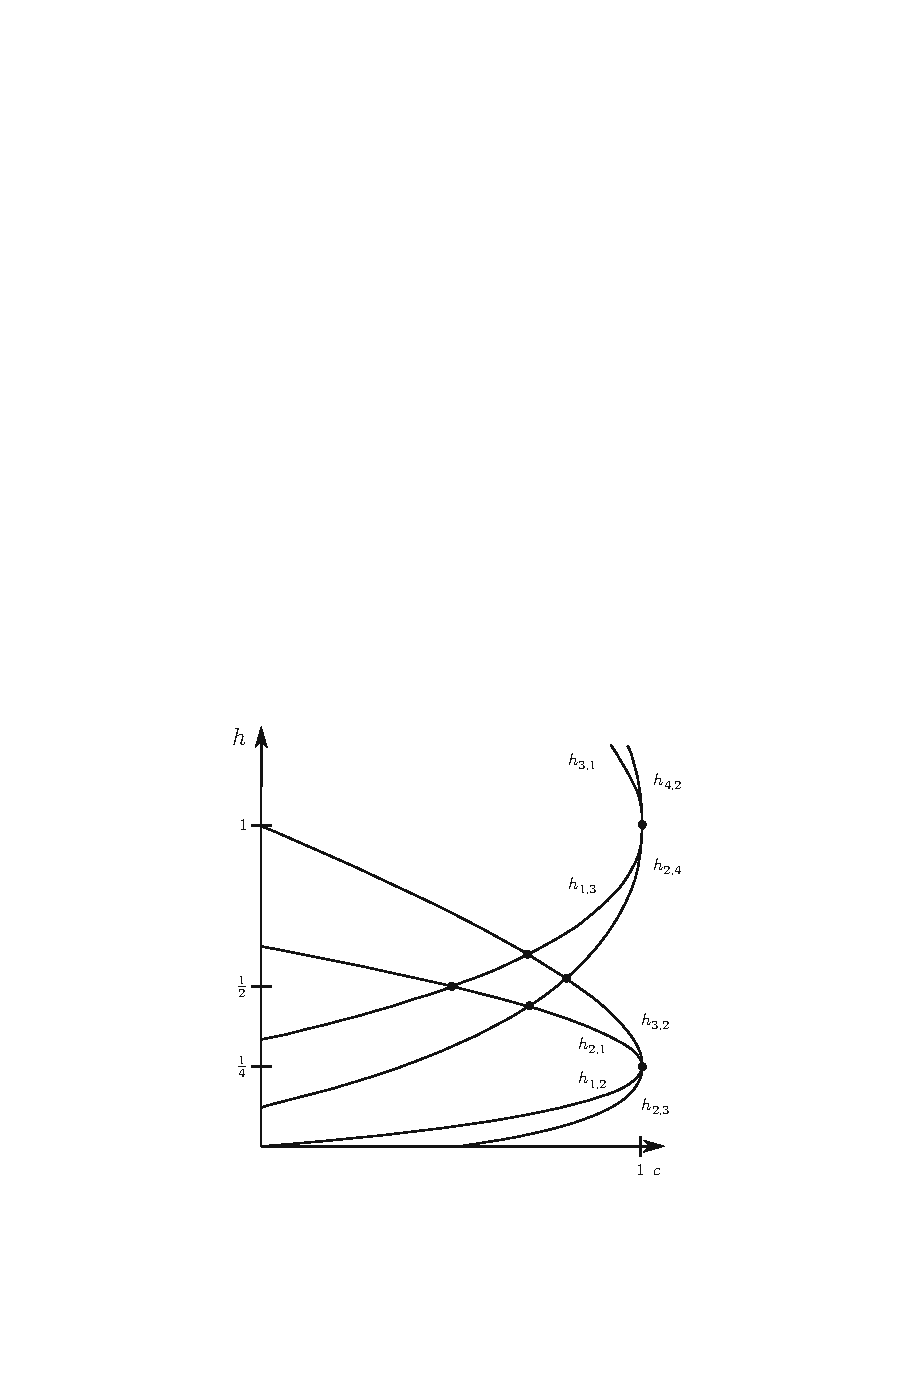
\includegraphics{figs/fig16.pdf}
	\label{unitary}
	\caption{Ka\v{c}行列式零点和中心荷之间的关系}
\end{figure}
\begin{itemize}
	\item $c>1,h> 0$:Ka\v{c}行列式无零点且其本征值都是正的,这个时候理论总是幺正
	\item $c=1$:Ka\v{c}行列式零点分布为$h=\frac{n^2}{4},n\in\mathbb{Z}$
	\item $c<1,h\geq 0$:只有图\ref{unitary}的交点处才会出现幺正表示
\end{itemize}
下面的定理给出了交点处的坐标:
\begin{theorem}[Unitary Minimal Models]
	$c<1,h\geq 0$的CFT,只有在中心荷满足:
	\begin{equation}
	\boxed{
			c=1-\frac6{m(m+1)}\quad m=3,4,\ldots
	}
	\end{equation}
	时才有幺正谱,谱为:
	\begin{equation}
		\boxed{
			h_{p,q}(m)=\frac{\left(\left(m+1\right)p-mq\right)^2-1}{4m\left(m+1\right)},\quad 1\leq p\leq m-1\mathrm{~and~}1\leq q\leq m
		}
	\end{equation}
\end{theorem}
我们原先说CFT的谱是无穷多或者连续的,但对于对称性只有Virasoro的CFT,幺正性直接让理论的谱变成有限离散的。这时的CFT我们称为\textbf{unitary minimal models}。有些时候理论不必是幺正的,不过我们还是希望这个CFT的谱依旧被限制为有限离散谱,这时的CFT称为\textbf{Minimal models},由下面的中心荷和谱定义:
\begin{theorem}[Minimal models]
	\begin{equation}
		\boxed{
			\begin{gathered}
				c=1-6\frac{(p-q)^2}{pq},\quad p,q\geq2,\quad p\perp q\\
			h_{r,s}(p,q)=\frac{(pr-qs)^2-(p-q)^2}{4pq},\quad 1\leq r\leq q-1\text{ and }1\leq s\leq p-1
			\end{gathered}
		}
	\end{equation}
\end{theorem}
类似这种谱有限离散,而且这时$h$还都是有理数的CFT我们称为\textbf{有理CFT(RCFT)}。
\begin{example}
	考虑$m=3$的幺正极小模型,这实际上是Ising Model二阶相变临界点处的理论,根据公式可以计算出中心荷为$\frac{1}{2}$,谱为:
	\begin{table}[H]
		\centering
		\renewcommand{\arraystretch}{1.5}
			\begin{tabular}{|c|c|}
				\hline
				$\frac{1}{2}$  & 0              \\ \hline
				$\frac{1}{16}$ & $\frac{1}{16}$ \\ \hline
				0              & $\frac{1}{2}$  \\ \hline
			\end{tabular}
		\caption{Ising模型的谱,横轴表示$1\leq p\leq 2$,纵轴表示$1\leq q\leq 3$}
	\end{table}
	从$p,q$取值范围来看似乎有$m(m-1)$个谱,但实际上有一半是重复的,只有$\mathrm{C}^2_m$个谱。
\end{example}

\section{Fusion Rules}
让我们从一个例子出发,利用\ref{33.31}
\begin{equation}
	\widehat{L}_{-2}\left.\phi(z)-\frac3{2\left(2h+1\right)}\widehat{L}_{-1}^2\right.\phi(z)=\left(\mathcal{L}_{-2}-\frac3{2\left(2h+1\right)}\mathcal{L}_{-1}^2\right)\left\langle\phi(w)\left.\phi_1(w_1)\ldots\phi_N(w_N)\right\rangle\right. =0
\end{equation}
得到微分方程:
\begin{equation}\label{37.2}
	\boxed{
		\left(\sum_{i=1}^N\left(\frac{h_i}{(w_i-w)^2}-\frac{1}{w_i-w}\partial_{w_i}\right)-\frac{3}{2(2h+1)}\partial_w^2\right)\left\langle\phi(w)\phi_1(w_1)\ldots\phi_N(w_N)\right\rangle=0
	}
\end{equation}
前面用共形对称性已经确定两点和三点函数只差一个常数系数,带入到方程中发现第一个non-trival的结果来自于三点函数:
\begin{equation}
	2\left(2h+1\right)\left(h+2h_2-h_1\right)=3\left(h-h_1+h_2\right)\left(h-h_1+h_2+1\right)
\end{equation}
$h,h_1,h_2$分别是$\phi,\phi_1,\phi_2$对应的共形权。这对三点函数的$C_{\phi\phi_1\phi_2}$做出了更强的限制,告诉我们绝大部分都是0。当然这个限制仅限于$h=h_{2,1}(m) \text{ or } h_{1,2}(m)$,这时上面的推导才成立,但是$h_1,h_2$是一般的。不妨取$h=h_{2,1}$,并把$h_1$也取为存在Null State的谱$h_{p,q}$,根据上面的方程可以解出不为0的条件是:
\begin{equation}
	h_2=\frac16+\frac h3+h_1\pm\frac23\sqrt{h^2+3hh_1-\frac12h+\frac32h_1+\frac1{16}}\in\{h_{p-1,q}(m),h_{p+1,q}(m)\}
\end{equation}
由OPE的一般表达式我们知道OPE是由一系列初级场和其导数,或者说次级场组合而成的,由于OPE有结合律,所以三点函数的计算可以看作是前两个先插入OPE\sn{我们假设第三个场隔得比较远,使得OPE的插入是精确的},然后和第三个场做两点函数,而两点函数不为零当且仅当共形权一致。上面的方程告诉我们三点函数不为零的条件是$h_2$只能取特定的两个值,从OPE去看这正说明了前两个场的OPE最终出来的那些场只能是共形权为$\{h_{p-1,q}(m),h_{p+1,q}(m)\}$的场的线性组合!这一思想完全可以推广到次级场的OPE:
\begin{equation}
	\begin{bmatrix}\phi_{(2,1)}\end{bmatrix}\times\begin{bmatrix}\phi_{(p,q)}\end{bmatrix}=\begin{bmatrix}\phi_{(p+1,q)}\end{bmatrix}+\begin{bmatrix}\phi_{(p-1,q)}\end{bmatrix}
\end{equation}
也就是说,$\phi_{(2,1)}$和$\phi_{(p,q)}$ Conformal family中的元素做OPE,最终得到的只能是$\phi_{(p-1,q)}$和$\phi_{(p+1,q)}$ Conformal family中元素的组合。
\begin{theorem}[Fusion rules of unitary minimal models]
	\begin{equation}
		\boxed{
			\left[\phi_{(p_1,q_1)}\right]\times \left[\phi_{(p_2,q_2)}\right]=\sum^{p_1+p_2-1}_{\begin{subarray}{l}
					k=1+|p_1-p_2|\\k+p_1+p_2\mathrm{~} \text{odd}\end{subarray}}\sum^{q_1+q_2-1}_{\begin{subarray}{l}
					l=1+|q_1-q_2|\\l+q_1+q_2\mathrm{~} \text{odd}\end{subarray}}\left[\phi_{(k,l)}\right]
		}
	\end{equation}
\end{theorem}
只要是RCFT,谱是离散有限的,都可以构造类似的融合规则:
\begin{equation}
	\boxed{
		[\left.\phi_i\right.]\times[\left.\phi_j\right.]=\sum_kN_{ij}^k\left[\left.\phi_k\right.\right],\quad N_{ij}^k\in\mathbb{Z}^+_0
	}
\end{equation}
根据OPE的性质可以知道这是一个交换代数,还是一个结合代数,其中的恒等元$[1]$就是Verma Module,对应真空表示,毕竟本身某个初级态的次级态就是用$N(T\cdots)$定义出来的。
\begin{theorem}
	\begin{equation}
		\boxed{
			\sum_lN_{kj}^lN_{il}^m=\sum_lN_{ij}^lN_{lk}^m
		}
	\end{equation}
	定义$(\overline{N}_i)_{jk}\equiv N_{ij}^k$,上式可以写成矩阵形式:
	\begin{equation}
		\boxed{
			\overline{N}_i\overline{N}_k=\overline{N}_k\overline{N}_i
		}
	\end{equation}
\end{theorem}
\begin{proof}
	证明就是使用交换律和结合律:
	\begin{equation}
		\begin{aligned}&\left[\phi_i\right]\times\left(\left[\phi_j\right]\times\left[\phi_k\right]\right)=\left[\phi_i\right]\times\sum_{l}N_{jk}^{l}\left[\phi_l\right]=\sum_{l,m}N_{jk}^{l}N_{il}^{m}\left[\phi_m\right]\\&\left(\left[\phi_i\right]\times\left[\phi_j\right]\right)\times\left[\phi_k\right]=\sum_{l,m}N_{ij}^{l}N_{lk}^{l}\left[\phi_m\right],\end{aligned}
	\end{equation}
\end{proof}
\subsection{Ising Model}

\section{Ka\v{c}\mbox{–}Moody Symmetry}
从现在开始,我们来考虑比Virasoro对称性更大的对称性。本节大量涉及无穷维李代数的艰深数学内容,大黄书专门用了两章进行铺垫介绍,这里不追求数学上的严谨性。\sn{数学读物可见\cite{Fuchs:1997af,Kac:1990gs}}
\subsection{Ka\v{c}\mbox{–}Moody Algebras}
Ka\v{c}\mbox{–}Moody对称性是理论中加入了其他守恒流,这些守恒流的洛朗模之间满足下面的代数关系:
\begin{definition}[Ka\v{c}\mbox{–}Moody Algebras]
	\begin{equation}\label{38.1}
		\boxed{
			\left[j_m^a,j_n^b\right]=i\sum_cf^{abc}j_{m+n}^c+k m\delta^{ab}\delta_{m+n,0}
		}
	\end{equation}
	$k$称为这个代数的level。
\end{definition}
从上面的定义看到$\{j_0^a\}$构成了上面这个代数的子代数,没有中心荷:
\begin{equation}\label{38.2}
	\left[j_0^a,j_0^b\right]=i\sum_cf^{abc}j_0^c
\end{equation}
这就是我们熟悉的李代数结构$\mathfrak{g}$,而Ka\v{c}\mbox{–}Moody代数可以看作是这个子代数的仿射化,记为$\hat{\mathfrak{g}}_k$。比如\ref{35.37}就是一个$\widehat{\mathfrak{su}}(2)_{1}$的代数结构。
\begin{theorem}[OPEs of Currents]
	由于OPE和对易关系蕴含完全相同的信息,所以前面的对易关系也可以翻译为流之间的OPE:
	\begin{equation}\label{38.3}
		\boxed{
			j^a(z)j^b(w)=\frac {k\delta^{ab}}{(z-w)^2}+\sum_c\frac{if^{abc}}{z-w}~j^c(w)+\cdots 
		}
	\end{equation}
\end{theorem}

\subsection{Sugawara Construction}
构造CFT首先要给出理论的谱,这可以通过寻找Ka\v{c}\mbox{–}Moody代数的表示得到,这个后面再说。理论在无穷小共形变换时的性质完全由能动张量刻画,本节的目的就是完全从自洽性出发把能动张量构造出来。

这些流是守恒流,就像我们构造Casimir算符一样,可以做下面的ansatz:
\begin{equation}
	T(z)=\gamma\sum_{a=1}^{\dim\mathfrak{g}}N\bigl(j^aj^a\bigr)(z)
\end{equation}
把所有的流加起来使得其再对称群变换下是不变的,现在根据$j^a$的共形权为$1$定出前面的归一化系数。
\begin{equation}
	L_m=\gamma\sum_{a=1}^{\dim\mathfrak{g}}\left(\sum_{l\leq-1}j_l^aj_{m-l}^a+\sum_{l>-1}j_{m-l}^aj_l^a\right)
\end{equation}
计算对易关系\footnote{计算中第四个等号利用了结构张量前两个指标反对称所导出的:
\begin{equation*}
	\begin{aligned}\sum_{l\leq-1}\left(j_l^bj_{m+n-l}^c-j_{l+n}^bj_{m-l}^c\right)&=\sum_{l\leq-1}j_l^bj_{m+n-l}^c-\sum_{l\leq-1+n}j_l^bj_{m+n-l}^c=-\sum_{l=0}^{n-1}j_l^bj_{m+n-l}^c\\\sum_{l>-1}\left(j_{m+n-l}^cj_l^b-j_{m-l}^cj_{l+n}^b\right)&=\sum_{l>-1}j_{m+n-l}^cj_l^b-\sum_{l>-1+n}j_{m+n-l}^cj_l^b=+\sum_{l=0}^{n-1}j_{m+n-l}^cj_l^b\end{aligned}
	\end{equation*}}:\sn{你依旧可以用OPE做}
\begin{align*}
		&[L_m,j_n^a]\\
		=&\gamma\sum_b\left(\sum_{l\leq-1}\left[j_l^bj_{m-l}^b,j_n^a\right]+\sum_{l>-1}\left[j_{m-l}^bj_l^b,j_n^a\right]\right) \\
		=&\gamma\sum_b\left(\sum_{l\leq-1}\left(j_l^b\bigl[j_{m-l}^b,j_n^a\bigr]+\bigl[j_l^b,j_n^a\bigr]j_{m-l}^b\right)+\sum_{l>-1}\left(j_{m-l}^b\bigl[j_l^b,j_n^a\bigr]+\bigl[j_{m-l}^b,j_n^a\bigr]j_l^b\right)\right) \\
		=&-2\gamma nkj_{m+n}^{a}+\gamma\sum_{b,c}if^{bac}\sum_{l\leq-1}\big(j_{l}^{b}j_{m+n-l}^{c}+j_{l+n}^{c}j_{m-l}^{b}\big) \\
		&+\gamma\sum_{b,c}if^{bac}\sum_{l>-1}\bigl(j_{m+n-l}^{c}j_{l}^{b}+j_{m-l}^{b}j_{l+n}^{c}\bigr)\\%换页\displaybreak
		=&-2\gamma nkj_{m+n}^a-\gamma\sum_{b,c}if^{bac}\sum_{l=0}^{n-1}[j_l^b,j_{m+n-l}^c] \\
		=&-2\gamma nkj_{m+n}^a-\gamma\sum_{b,c}if^{bac}\sum_{l=0}^{n-1}\sum_dif^{bcd}j_{m+n}^d \\
		=&-2\gamma nkj_{m+n}^a+\gamma n\sum_{b,c,d}f^{bac}f^{bcd}j_{m+n}^d. 
\end{align*}
李代数的伴随表示有下面的等式:
\begin{equation}\label{38.6}
	\sum_{b,c}f^{bac}f^{bcd}=-2C_{\mathfrak{g}}\delta^{ad}
\end{equation}
其中$C_{\mathfrak{g}}$叫\textbf{dual Coxeter number},下表给出了一些李群的dual Coxeter number:
\begin{table}[H]
	\centering
	\begin{tabular}{|c|c|c|c|c|c|}
		\hline
		Algebar        & $A_n$ & $D_n$  & $E_6$ & $E_7$ & $E_8$ \\ \hline
		$C_{\mathfrak{g}}$ & $n+1$ & $2n-2$ & $12$  & $18$  & $30$  \\ \hline
	\end{tabular}
	\caption{ADE分类的Coxeter number,在现在的语境下可以将$A_n$对应$\mathfrak{su}_{n+1}$,$D_n$对应$\mathfrak{so}_{2n}$}
\end{table}
\begin{theorem}[Sugawara energy–momentum tensor]
	$\hat{\mathfrak{g}}_k$所确定CFT的能动张量由下式给定:
	\begin{equation}\label{38.7}
		\boxed{
			T(z)=\frac1{2\left(k+C_{\mathfrak{g}}\right)}\sum_{a=1}^{\dim\mathfrak{g}}N\left(j^aj^a\right)(z)
		}
	\end{equation}
\end{theorem}
利用能动张量OPE或者$\frac c2=\left\langle0\right|L_{+2}L_{-2}\left|0\right\rangle $可计算出理论的中心荷:
\begin{theorem}
	Sugawara构造出来的CFT中心荷为:
	\begin{equation}
		\boxed{
			c=\frac{k\dim\mathfrak{g}}{k+C_{\mathfrak{g}}}
		}
	\end{equation}
\end{theorem}
\subsection{WZNW Models}
前面导出能动张量的过程再次强调了研究CFT时很多情况下拉氏量是放在次要位置的,我们当然也可以直接构造一个有流对称代数的拉氏量,即所谓的WZW模型,然后再用作用量变分导数得到能动张量。本节目的是知道这样做有多麻烦。

从自由玻色场来看,其作用量可以写成下面的形式:\sn{已重新选取耦合常数}
\begin{equation}
	\mathcal{S}=\frac1{8\pi}\int_\Sigma\mathrm{d}^2x\partial^\mu g^{-1}\partial_\mu g=\frac1{8\pi}\int_\Sigma\mathrm{d}^2x\partial g^{-1}\overline{\partial}g
\end{equation}
这里$\Sigma$是复平面这个最简单的黎曼曲面,其中$g$是:
\begin{equation}
	g:\mathbb{C}\to\mathcal{U}(1);z\mapsto g(z,\overline{z})=\exp(i\varphi(z,\overline{z}))
\end{equation}
前面说$\phi\mapsto\phi+a$是$U(1)$对称性或许还有些困惑,从这个作用量就很好看出来的确是$g\mapsto e^{ia} g$的$U(1)$变换,WZNW模型就是对这个模型的非阿贝尔推广。
\subsubsection{Nonlinear Sigma Models}
\begin{definition}
	非线性sigma模型包含一个定义在某个黎曼曲面上的到群流形的玻色场$g:\Sigma\to G$\footnote{或者精确点说是在$G$的幺正表示里面取值},作用量为:
	\begin{equation}
		\mathcal{S}_0=\frac1{2a^2}\int_\Sigma\mathrm{d}^2x\mathrm{~Tr}\left(\partial^\mu g^{-1}\partial_\mu g\right)
	\end{equation}
	这个$\mathrm{Tr}$其实要写成$\mathrm{Tr^\prime}$和一般的取迹进行区分,如果在某个表示下,生成元矩阵有$\mathrm{Tr}(t^a t^b)=x\delta^{ab}$,那么$\mathrm{Tr^\prime}\equiv\frac{1}{x}\mathrm{Tr}$。后面假设都已经做了这个归一化。
\end{definition}
对作用量进行变分得到运动方程:
\begin{equation}
	\partial^\mu(g^{-1}\partial_\mu g)=0
\end{equation}
这直接说明了存在下面的守恒流:
\begin{equation}
	J_\mu=g^{-1}\partial_\mu g
\end{equation}
这个守恒流对应模型的global $G\times G$对称性。黎曼曲面是一个一维复流形,任何一点领域都同胚于复平面的开子集,所以可以在上面local地赋予复坐标,定义上面守恒流的全纯和反全纯部分:
\begin{equation}
	J_z=g^{-1}\partial g,\quad\bar{J}_{\overline{z}}=g^{-1}\overline{\partial}g\Rightarrow\partial\bar{J}_{\overline{z}}+\bar{\partial}J_z=0
\end{equation}
一般而言,全纯和反全纯部分不能单独守恒,和$U(1)$的情况不一样,我们期望在理论中加上一些项,让对称性进一步扩大为反全纯和全纯部分单独守恒。
\begin{definition}[Wess-Zumino term]
	\begin{equation}
		\Gamma=\frac{-i}{12\pi}\int_B\mathrm{d}^3y\epsilon_{\alpha\beta\gamma}\operatorname{Tr}\left(\widetilde{g}^{-1}\partial^\alpha\widetilde{g}\widetilde{g}^{-1}\partial^\beta\widetilde{g}\widetilde{g}^{-1}\partial^\gamma\widetilde{g}\right)
	\end{equation}
	这里$B$是一个带边三维流行,其边界为$\Sigma$,$\tilde{g}: B\to G$可看作是$g$从Boundary到Bulk的扩张,这种扩张不是唯一的,流形$B$也不是唯一的。但可以证明这个差别只会体现为$2n\pi i$,所以虽然作用量上面看不一样,但是最终就欧几里得路径积分而言$e^{-\Gamma}$是唯一的,所以不会对场论造成任何影响。
\end{definition}
\subsubsection{Wess-Zumino-Novikov-Witten Models}
考虑下面的作用量:
\begin{equation}
	\mathcal{S}=\mathcal{S}_0+k\Gamma,\quad k\in\mathbb{Z}
\end{equation}
按照前面说的虽然$\Gamma$不唯一,但是理论唯一。计算运动方程为:
\begin{equation}
	\partial^\mu(g^{-1}\partial_\mu g)+\frac{a^2ik}{4\pi}\epsilon_{\mu\nu}\partial^\mu(g^{-1}\partial^\nu g)=0
\end{equation}
在复坐标下为:
\begin{equation}
	\left(1+\frac{a^2k}{4\pi}\right)\partial(g^{-1}\overline{\partial}g)+\left(1-\frac{a^2k}{4\pi}\right)\overline{\partial}(g^{-1}\partial g)=0
\end{equation}
所以为了让流的全纯和反全纯部分的流单独守恒,要求:
\begin{equation}
	a^2=4\pi/k
\end{equation}
\begin{theorem}[$\widehat{\mathfrak{g}}_k$ WZNW Models]
	\begin{equation}
		\mathcal{S}=\frac k{8\pi}\int_\Sigma\mathrm{d}^2x\mathrm{~Tr}\left(\partial^\mu g^{-1}\partial_\mu g\right)+k\Gamma ,\quad k\in\mathbb{Z}^+
	\end{equation}
\end{theorem}
另外一个$a^2=-4\pi/k$的解并不是我们关注的流守恒。左右流的单独守恒体现到场上是场可以分解为$g(z,\overline{z})=g_L(z)g_R(\overline{z})$,提现到体系的对称群上是从global $G\times G$扩张为local的$G(z)\times  G(\bar z)$,即下面的变换下作用量不变:
\begin{equation}
	g(z,\bar{z})\to\Omega(z)g(z,\bar{z})\overline{\Omega}^{-1}(\bar{z}),\quad \Omega(z),\bar \Omega(\bar z)\in G
\end{equation}
rescale守恒流:
\begin{equation}
	\begin{aligned}
		{J(z)} &\equiv-\frac k2J_z(z)=-\frac k2\partial gg^{-1} \\
	\bar{J}(\overline{z}) &\equiv\frac k2\bar{J}_{\overline{z}}(\overline{z})=\frac k2g^{-1}\overline{\partial}g
	\end{aligned}
\end{equation}
然后类似于YM理论里面的操作,在生成元$t^a$上投影,$J=J^at^a$,可以证明$J^a$就是那些Ka\v{c}\mbox{-}Moody流,理论的能动张量也就是Sugawara构造的那样!

\subsection{Knizhnik\mbox{–}Zamolodchikov Equation}
前面我们研究初级场实际上都是在看其在Virasoro代数下如何变换,现在显然我们要找更大对称群的表示。就像是YM理论一样,除了Lorentz变换本身对场进行了分类,分成标量场,矢量场等等。然后理论中本身冒出来一个规范对称群,要求理论中不同的场$\phi_a$之间在$\phi_a\to U^{ab}_R\phi_b$的规范变换下理论仍不变。这种场之间的内在对称性实际上就类似于Ka\v{c}\mbox{-}Moody对称性,场除了被Virasoro表示分类(不同的共形权),还要在流代数的表示之中。
\begin{definition}[Ka\v{c}\mbox{–}Moody (chiral) primary field]
	\begin{equation}\label{kac}
		\boxed{
			j^a(z)\phi_R^r(w)=\frac1{z-w}\sum_s\left(t_R^a\right)_s^r\phi_R^s(w)+\cdots 
		}
	\end{equation}
	$j^a$是生成变换群$G$的流,$R$表示$\{\phi_R^a\}$具体处于群的哪个表示,$t^a_R$是生成元的表示矩阵。满足这一条件的初级场,一定也是Virasoro初级场,你可以尝试去计算Sugawara能动张量和$\phi$之间的OPE来证明这一点。
\end{definition}
\begin{remark}
	本节我们只考虑全纯部分,因为全纯反全纯完全解耦,把反全纯部分也加上来后初级场定义为:
	\begin{equation}
		\begin{aligned}&j^a(z)\phi_{R,\bar R}(w,\bar{w})\sim\frac{t_R^a\phi_{R,\bar R}(w,\bar{w})}{z-w}\\&\bar{j}^a(\bar{z})\phi_{R,\bar R}(w,\bar{w})\sim-\frac{\phi_{R,\bar R}(w,\bar{w})t_{{\bar R}}^a}{\bar{z}-\bar{w}}\end{aligned}
	\end{equation}
	$R,\bar R$分别表示全纯和反全纯部分处于哪个表示。另外,不少文献对\ref{kac}的定义差个负号,这会导致后面的方程正负号有些差别,但这无伤大雅。
\end{remark}
\subsection{Ward Identity for Ka\v{c}\mbox{–}Moody Symmetries}
Virasoro初级场有Ward恒等式限制它们之间的关联函数形式,同样这里也有更强的限制:
\begin{theorem}
	\begin{equation}\label{38.11}
		\boxed{
			\begin{aligned}
				\left<j^{a}(z)\phi_{R_{1}}(w_{1},\overline{w}_{1})\right.& \ldots\phi_{R_N}(w_N,\overline{w}_N)\rangle   \\
				&=\sum_{i=1}^N\frac{t_{R_i}^a}{z-w_i}\left\langle\left.\phi_{R_1}(w_1,\overline{w}_1)\ldots\phi_{R_N}(w_N,\overline{w}_N)\right.\right\rangle +\text{regular}
			\end{aligned}
		}
	\end{equation}
	这里$\{\phi_{R_i}\}$是Ka\v{c}\mbox{–}Moody (chiral) primary field,$t_{R_i}$仅仅作用于$\phi_{R_i}$,它们的矩阵指标没有明写出来。
\end{theorem}
\begin{proof}
	证明过程和共形Ward恒等式的证明一模一样,守恒流给出守恒荷从而给出Ka\v{c}\mbox{-}Moody代数作用下场的无穷小变换的形式:
	\begin{equation}
		-\delta_\epsilon\phi(w)=\oint_{\mathcal{C}(w)}\frac{dz}{2\pi i}\sum_a\left.j^a(z)\right.\epsilon^a(z)\phi(w)
	\end{equation}
	考虑关联函数的无穷小变换:
	\begin{equation}
		\begin{aligned}
			&\delta_{\epsilon}\left\langle\phi_{R_{1}}(w_{1},\overline{w}_{1})\ldots\phi_{R_{N}}(w_{N},\overline{w}_{N})\right\rangle  \\
			&=\oint_{\mathcal{C}(w_1,...,w_N)}\frac{dz}{2\pi i}\sum_a\epsilon^a(z)\Big\langle j^a(z)\phi_{R_1}(w_1,\overline{w}_1)\ldots\phi_{R_N}(w_N,\overline{w}_N)\Big\rangle  \\
			&=\sum_{i=1}^N\oint_{\mathcal{C}(w_i)}\frac{dz}{2\pi i}\sum_a\epsilon^a(z)\big<\phi_{R_1}(w_1,\overline{w}_1)\ldots\bigg(j^a(z)\phi_{R_i}(w_i,\overline{w}_i)\bigg)\ldots\phi_{R_N}(w_N,\overline{w}_N)\big>\\
			&=\sum_{i=1}^N\oint_{\mathcal{C}(w_i)}\frac{dz}{2\pi i}\sum_a\epsilon^a(z)\frac{t_{R_i}^a}{z-w_i}\left\langle\phi_{R_1}(w_1,\overline{w}_1)\ldots\phi_{R_N}(w_N,\overline{w}_N)\right\rangle
		\end{aligned}
	\end{equation}
	比较第一个等号和最后一个等号即得证。由于上面的关联函数在$G$的global作用下实际上要不变,所以上面这一长串等式,\textbf{在$\epsilon$为常数时},实际上为0,所以我们其实还有下面的等式成立:\footnote{证明的前一半是local形式的证明,因为证明中群变换的参数$\epsilon$是local的,所以才能说积分号里面的东西相等;证明global的形式实际上是让$\epsilon$是global的参数,也就是考虑global的群变换,这部分才是对称性,由于$\epsilon$与$z$无关,所以上式最后一个等式可以把围道积分积出来得到下式。\ref{31.37}也可以用这种方式来看。}
	\begin{equation}
		\boxed{
			\sum_{i=1}^nt_i^a\left<\phi_1(z_1)\cdots\phi_n(z_n)\right>=0
		}
	\end{equation}
	这个等式类似于\ref{31.37},确定了两点和三点函数。
\end{proof}
\subsection{Ka\v{c}\mbox{–}Moody descendant fields}
从态的角度看,现在对称性增大了,原先构造descendant fields是用Virasoro初级场配合$L_{-n},n\geq 1$去构造,现在初级场应该用Ka\v{c}\mbox{–}Moody初级场,产生算符应该用对称性所对应的$j_{-n},n\geq 1$\footnote{现在估计就不难从数学上去理解我们为什么构造Free Bosons的希尔伯特空间的时候是用$j_{-n}$去构造了,因为理论是$\hat{\mathfrak{u}}(1)$的对称性,所以我们希望初级场是Ka\v{c}\mbox{-}Moody的,次级态也是,所以$j_{-n}$作用真空上去得到Verma模,作用到顶点算符构造的初级场上面得到次级态($jV_\alpha$的OPE确实有\ref{kac}的形式,$U(1)$还是过于trivial,生成元表示就是一个常数。)。由于$T$就是用$j$ Sugawara构造来的,所以也同时是Virasoro初级态。}。\sn{下面的$\mathcal{U}(\hat{g}_k)$不少文献称为$\hat{g}_k$的泛包络代数的表示,名字很唬人,简单点说就是那些$j^a_{-n}$构成的一个结合代数,也就是$j^a_{-n}j^b_{-m}\ldots$,下标$+$表示只取$n\geq 1$。}
\[\text{Ka\v{c}\mbox{–}Moody descendant fields} = \{\mathcal{U}(\hat{g}_k)_+\ket{\phi_R}\}\]
同样类似\ref{eq:33.30}态算符对应给出次级场:
\begin{equation}
	\boxed{
		(\widehat{j}_{-n}^a\phi_R)(w)=\oint_{\mathcal{C}(w)}\frac{dz}{2\pi i}\frac1{(z-w)^n}j^a(z)\phi_R(w)
	}
\end{equation}
\begin{example}
	\begin{equation}
		\begin{aligned}
			j_0^a\left|\phi_R\right\rangle & =\lim\limits_{w\to0}\oint\frac{dz}{2\pi i}j^{a}(z)\phi_{R}(w)\big|0\big>  \\
			&=\lim_{w\to0}\oint\frac{dz}{2\pi i}\left(\frac1{z-w}t_R^a\phi_R(w)+\cdots\right)\left|0\right\rangle=t_R^a\left|\phi_R\right\rangle 
		\end{aligned}
	\end{equation}
	这个方程蛮重要的,它告诉我们$\phi_R$生成了$j_0$的表示空间而$j_0$就是没有仿射化的,通常的李代数\ref{38.2}的群表示,一下就看清楚了$\phi_R$这个下标$R$的具体意义。而对称性变大之后,最高权除了由$L_0$本征值$h$标记,还应该由$j_0^a$所处的表示来标记,后面用例子来感受这一点。
\end{example}
利用这个我们可以类似去计算Ka\v{c}\mbox{–}Moody descendant fields和Ka\v{c}\mbox{–}Moody primary fields之间的关联函数,有与\ref{33.31}类似的方程:
\begin{theorem}
	\begin{equation}\label{38.15}
		\boxed{
			\begin{gathered}
				\left\langle\widehat{j}_{-n}\phi_R(w)\phi_{R_1}(w_{1})\ldots\phi_{R_N}(w_{N})\right\rangle=\mathcal{J}_{-n}\langle\phi_R(w)\phi_{R_1}(w_{1})\ldots\phi_{R_N}(w_{N})\rangle  \\
				\text{Where,}\qquad\mathcal{J}_{-n}=-\sum_{i=1}^N\frac{t^a_{R_i}}{(w_i-w)^n}
			\end{gathered}
		}
	\end{equation}
\end{theorem}

更关键的是去找理论中的零模,从而得到类似\ref{37.2}的对初级场关联函数约束。
\begin{theorem}[Knizhnik–Zamolodchikov Equation]
	\begin{equation}\label{KZ}
		\boxed{
			\left(\partial_{w_i}-\frac{1}{k+C_{\mathfrak{g}}}\sum_{j\neq i}\left.\frac{\sum_{a}t_{R_i}^{a}\otimes t_{R_j}^{a}}{w_i-w_j}\right)\big\langle\phi_{R_1}(w_1)\ldots\phi_{R_N}(w_N)\big\rangle=0\right.
		}
	\end{equation}
	上式省略了矩阵下标,$t^a_{R_i}$只作用于$\phi_{R_i}$。上面方程对任意的$i=1,\ldots,N$都成立。
\end{theorem}
\begin{proof}
	\begin{equation}
		\begin{aligned}
			L_{-1}\left|\phi_{R}^{r}\right\rangle & =\frac1{2\left(k+C_{\mathfrak{g}}\right)}\sum_a\left(\sum_{l\leq-1}j_l^aj_{-1-l}^a+\sum_{l>-1}j_{-1-l}^aj_l^a\right)\ket{\phi_R^r}  \\
			&=\frac1{2\left(k+C_{\mathfrak{g}}\right)}\sum_a\left(j_{-1}^aj_0^a+j_{-1}^a j_0^a\right)\ket{\phi_R^r}\\
			&=\frac1{k+C_{\mathfrak{g}}}\sum_aj_{-1}^a\sum_s{\left(t_R^a\right)^r}_s\ket{\phi_R^r},
		\end{aligned}
	\end{equation}
	直接给出了一个Null State:
	\begin{equation}
		\left(\widehat{L}_{-1}-\frac1{k+C_{\mathfrak{g}}}\sum_a\widehat{j}_{-1}^at_R^a\right)\phi_R(z)=0
	\end{equation}
	这可以看作是Sugawara构造用次级态表述。把它插在关联函数中恒为0:
	\begin{equation}
		0=\left\langle\phi_{R_1}(w_1)\ldots\left(\widehat{L}_{-1}-\frac1{k+C_{\mathfrak{g}}}\sum_a\widehat{j}_{-1}^at_{R_i}^a\right)\phi_{R_i}(w_i)\ldots\phi_{R_N}(w_N)\right\rangle 
	\end{equation}
	再利用\ref{33.31}和\ref{38.15}即可证明。
\end{proof}
注意这个约束非常一般,前面\ref{37.2}好歹还要求$\ket{h}$本身就是有零模的谱,对$h$有约束,这里就啥也没有了。KZ方程的解催生出了非常多的数学问题,由于四点函数不能被共形对称性很好的确定,所以我们比较关心这个方程能否给出四点函数的形式?文章\cite{Knizhnik:1984nr}在末尾用合流超几何函数给了答案。
\begin{remark}
	本节前面的讨论相当于选取了一个特殊的基底,\ref{38.6}更一般的表述是下面的Killing型:
	\begin{equation}
		K^{ab}=\frac1{2g}\operatorname{Tr}\left(\operatorname{ad}_{t^a}\operatorname{ad}_{t^b}\right)=\frac1{2g}f^{acd}f^{bdc}
	\end{equation}
	前面我们在$\mathfrak{g}$中shift基底将$K_{ab}$化为$\delta_{ab}$,\ref{38.1}、\ref{38.3}、\ref{38.7}和\ref{KZ}的形式都要发生相应的变化,具体来说就是$\delta^{ab}\to K_{ab}$,注意$J^aJ^a$中隐含了一个$\delta_{ab}$。
\end{remark}

\section{Example: Highest Weight Representations of $\widehat{\mathfrak{su}}(2)_{k}$ }
 $\widehat{\mathfrak{su}}(2)_{k}$流代数和我们熟悉的角动量系统非常接近,首先按照下面的方式构造出流中的上升下降算符:
 \begin{equation}
 	\hat{j}_m^3=\frac1{\sqrt{2}}~j_m^3~,\quad\quad\hat{j}_m^\pm=\frac1{\sqrt{2}}~\left(j_m^1\pm i~j_m^2\right)
 \end{equation}
满足对易关系:
\begin{equation}
	\left[\hat{j}_m^3,\hat{j}_n^3\right]=\frac{mk}2\delta_{m+n,0},\quad\left[\hat{j}_m^3,\hat{j}_n^\pm\right]=\pm\hat{j}_{m+n}^\pm,,\quad\left[\hat{j}_m^+,\hat{j}_n^-\right]=km\delta_{m+n,0}+2\hat{j}_{m+n}^3
\end{equation}
前面就提到过$\{j_0\}$生成无中心荷的$\mathfrak{su}(2)$子代数,而且不难看到$L_0$和他们是对易的,所以现在$L_0$的$h$模是简并的,简并态构成的子空间是$\mathfrak{su}(2)$子代数的表示空间,这个表示空间还不只有一个不等价不可约表示,可能是很多不等价不可约表示直和起来构造出的更大的空间。所以现在最高权应该有两个指标标记,一个指标是其共形权$h$,表示其能量$L_0$,最高的含义依旧是:
\begin{equation}
	L_0\ket{h}=h\ket{h,q},\quad L_n\ket{h,q}=0,\quad \forall n>0
\end{equation}
第二个标记$q$是在说其处于哪个$\mathfrak{su}(2)$的表示,$\mathfrak{su}(2)$群的表示可以用自旋$l=0,\frac{1}{2},1,\ldots$去标记,而我们这里关心的是最高权,所以它在$\mathfrak{su}(2)$的表示中也是最高的那个,也就是$m=l$,这里我们设$q=2l\in\mathbb{Z}^+_0$。另外它作为最高权还要类似$L_{-n}$湮灭一样被$j^a_{-n}$湮灭:
\begin{equation}
	\begin{aligned}\hat{j}_n^3\left|h,q\right\rangle&=\hat{j}_n^\pm\left|h,q\right\rangle=0\quad\text{for }n>0\\\hat{j}_0^3\left|h,q\right\rangle&=\frac{q}{2}\left|h,q\right\rangle,\\\hat{j}_0^+\left|h,q\right\rangle&=0.\end{aligned}
\end{equation}
这些条件合起来就定义了一个最高权表示,与Virasoro代数不同,初级态不止包含这些最高权,实际上它应该包含所有$h$模简并的态,或者说我们要用$\hat {j}_0^\pm$继续在$\mathfrak{su}(2)$的自旋$q/2$表示中升降把表示空间构造全:\sn{再次强调按照定义这些$\alpha\neq 0$的态不是最高权,它们在$\mathfrak{su}(2)$的表示下不是最高的。}
\begin{equation}
	\left|h,q_\alpha\right\rangle:=\left(\hat{j}_0^-\right)^\alpha\left|h,q\right\rangle ,\quad \alpha =0,1,2,\ldots,q
\end{equation}
这就对应于前面Ka\v{c}\mbox{-}Moody初级场的$\ket{h,q_\alpha}$,显然从这个构造就可以看出来$\ket{h,q_\alpha}$张成$\mathfrak{su}(2)$的一个表示。利用Sugawara构造得知:
\begin{equation}
	L_0=\frac1{2\left(k+2\right)}\sum_{a=1}^3\left(\sum_{l\leq-1}j_{+l}^aj_{-l}^a+\sum_{l>-1}j_{-l}^aj_{+l}^a\right)
\end{equation}
由此可计算$\ket{h,q}$关于$L_0$的本征值:
\begin{equation}
	\begin{aligned}
		L_{0}\left|h,q\right\rangle & =\frac1{2\left(k+2\right)}\sum_{a=1}^{3}j_{0}^{a}j_{0}^{a}\left|h,q\right\rangle   \\
		&=\frac1{k+2}\sum_{a=1}^3\hat{j}_0^a\hat{j}_0^a\left|h,q\right\rangle=\frac{q(q+2)}{4(k+2)}\left|h,q\right\rangle 
	\end{aligned}
\end{equation}
计算的最后利用了$j_0^aj_0^a$是$\mathfrak{su}(2)$的Casimir算符。但是我们又知道本征值应该为$h$,所以$L_0$的谱和允许的表示之间是有关联的,要求:
\begin{equation}
	\boxed{
		h=\frac{q(q+2)}{4(k+2)}
	}
\end{equation}
而$q\in\mathbb{Z}^+_0$,所以理论中的谱可取值被极大限制住了,这也再次说明了这个模型是个RCFT。上面做的这些实际上是在考虑$\widehat{\mathfrak{su}}(2)_k$的非常特殊的一个$\mathfrak{su}(2)$子群,其实这样的子群有无数多个$\mathfrak{su}(2)_{(n)}\subset\widehat{\mathfrak{su}}(2)_k$:\sn{\[\begin{aligned}
		&\left[L_0,\widetilde{j}^{\pm}_{(n)}\right]=\mp n\widetilde{j}^{\pm}_{(n)}\\
		&\left[\widehat{j}_0^3,\widetilde{j}^{\pm}_{(n)}\right]=\pm \widetilde{j}^{\pm}_{(n)}
	\end{aligned}\]
所以$h$的增加以1为单位,$q$的增加以2为单位}
\begin{equation}
	\boxed{
		\begin{aligned}
			&\widetilde{j}_{(n)}^+ =\frac1{\sqrt{2}}\left(j_{-n}^1+i~j_{-n}^2\right),  \\
			&\widetilde{j}_{(n)}^- =\frac1{\sqrt{2}}\left(j_{+n}^1-i~j_{+n}^2\right),  \\
			&\widetilde{j}_{(n)}^{3} =\frac1{\sqrt{2}}~j_0^3-\frac{n~k}2~, 
		\end{aligned}
	}
\end{equation}
首先考虑$\mathfrak{su}(2)_{(1)}$,计算$j^+_{(1)}\ket{h,q}$的模:
\begin{equation}
	\begin{aligned}
		\langle h,q\mid\tilde{j}^{-}_{(1)}\tilde{j}^{+}_{(1)}\big|h,q\big\rangle & =\langle h,q\mid\begin{bmatrix}\tilde{j}^-_{(1)},\tilde{j}^+_{(1)}\end{bmatrix}\big|h,q\big\rangle   \\
		&=\langle h,q\mid-2\tilde{j}^3\mid h,q\rangle  \\
		&=-2\bra{h,q}j_0^3-\frac k{2}\ket{h,q} \\
		&=-q+k
	\end{aligned}
\end{equation}
而我们如果考虑幺正表示,所有的谱模应当正定,所以$q\leq k$。
\begin{theorem}
	$\widehat{\mathfrak{su}}(2)_k$最高权表示幺正要求$\boxed{0\leq q\leq k}$。
\end{theorem}
我们只说明了必要性,请相信它也是充分的。现在考虑其他$\mathfrak{su}(2)_{(n)}$。现在考虑具体的$k=1$的简单情形,考虑$\ket{0,0}$这个最高权,反复作用$\widetilde{j}_{(n)}^\pm$去构造表示空间中的其它态,表示空间中的向量我们仍用本征值$h,q$标记,但是它们不是最高权,所以前面的一些约束都没有了。最高权表示对应的初级态$\ket{h,q_\alpha}$相对$\widetilde{\mathfrak{su}}(2)_{(0)}$处在自旋$q/2$表示中,自然想到把这些初级态作用$\widetilde{j}_{(n)}^\pm$之后应该是别的$\widetilde{\mathfrak{su}}(2)_{(n)}$子群的表示。

比如$\tilde{j}_{(1)}^3\ket{0,0}=-\frac{1}{2}\ket{0,0}$,而且$\tilde{j}_{(1)}^-\ket{0,0}=0$,所以$\{\ket{0,0},\tilde{j}_{(1)}^+\ket{0,0}=\ket{0,0}\}$处于$\widetilde{\mathfrak{su}}(2)_{(1)}$的自旋$1/2$表示,对应$(h,q)=\{(0,0),(1,2)\}$。

$\tilde{j}_{(2)}^3\tilde{j}_{(1)}^+|0,0\rangle =0$且$\tilde{j}_{(2)}^+\tilde{j}_{(1)}^+|0,0\rangle =0$,所以$\tilde{j}_{(1)}^+|0,0\rangle $又处在$\widetilde{\mathfrak{su}}(2)_{(2)}$的自旋$0$表示。$\{\tilde{j}_{(1)}^+|0,0\rangle ,\tilde{j}_{(3)}^{+}\tilde{j}_{(1)}^{+}|0,0\rangle \}$又张成$\mathfrak{su}(2)_{(3)}$的自旋$1/2$表示,对应$(h,q)=\{(0,0),(4,4)\}$。可见,由于这些不同$n$对应$\tilde{j}_{(n)}^\pm$的是不对易的,所以这些表示是以某种方式“纠缠”在一起的。这个过程可以无限进行下去,我们得到权图\ref{fig17}。
\begin{figure}
	\centering
	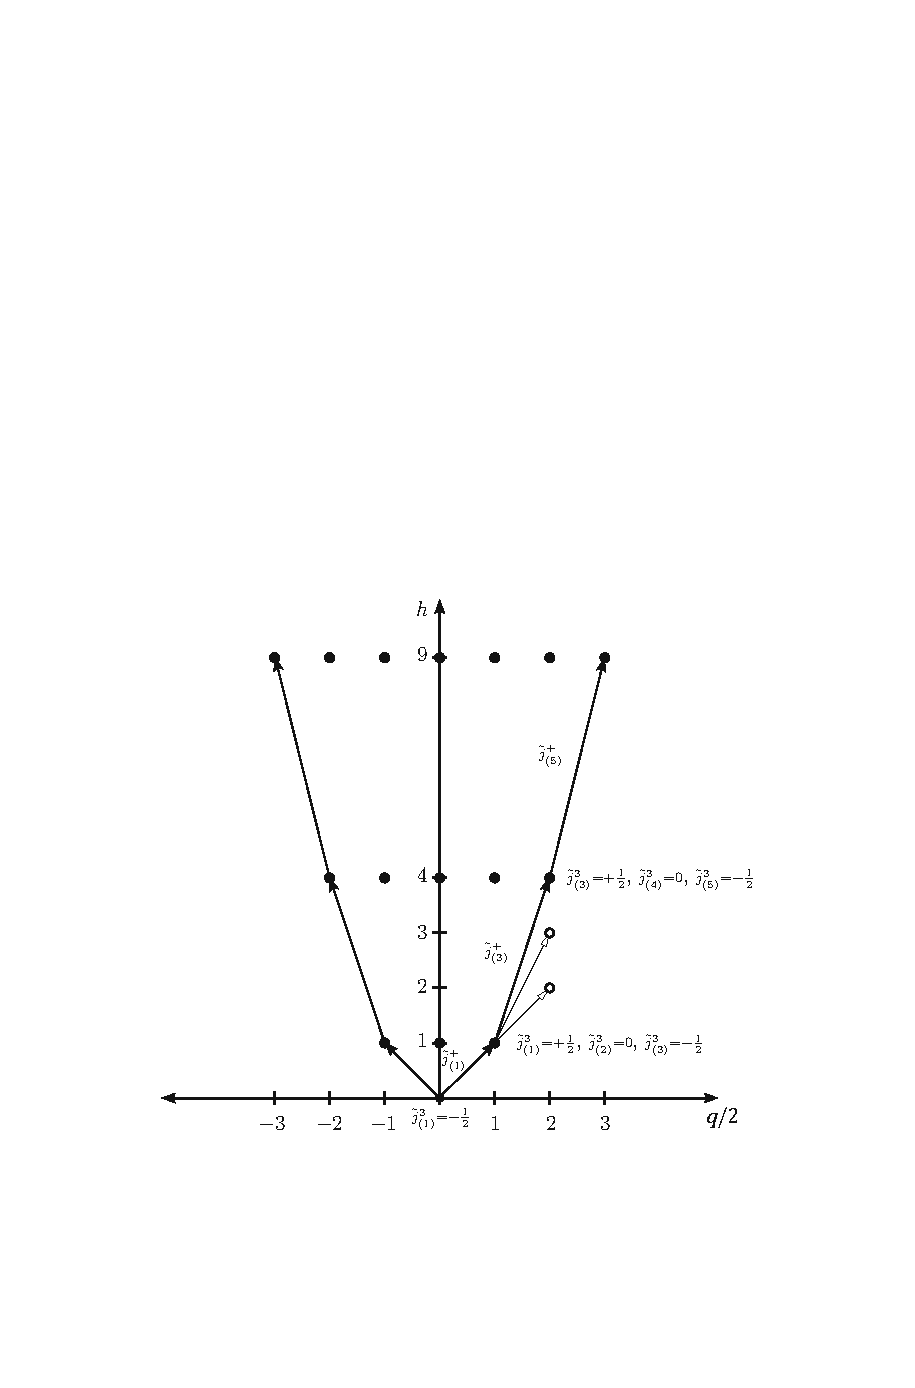
\includegraphics{figs/fig17.pdf}
	\caption{这些黑点表示作用$\widetilde{j}^\pm_{(n)}$可以得到的态,实心箭头表示用roots升降权,空心箭头表示作用任何一个root上去都得0}
	\label{fig17}
\end{figure}

这个权图是有边界的,边界为$(h,q)=(m^2,2m),m\in\mathbb{Z}$。这些边界才是真正要紧的,构造次级态就看它们,就$\widehat{\mathfrak{su}}(2)_1$而言,知道了边界的那些态,就足够构造整个希尔伯特空间,下面从玻色子的想法来说明。

玻色子体系是有$\widehat{\mathfrak{su}}(2)_1$代数的,具体而言可以由$R=\sqrt{2}$上的紧致化实现:\sn{后面的$(h,q)$表示场对应的态所对应的$L_0,\widehat{j}^3_0$本征值}
\begin{equation}
	\begin{aligned}j(z)&=i\partial X(z,\overline{z})&\left(h,q\right)&=\left(1,0\right),\\V_{\pm\sqrt{2}}&=:e^{\pm i\sqrt{2}X}:&\left(h,q\right)&=\left(1,\pm2\right)\end{aligned}
\end{equation}
前面提到过还应存在初级场:
\begin{equation}
	V_{\pm\sqrt{2}m}=:e^{\pm i\sqrt{2}mX}:\quad (h,q)=(m^2,\pm 2m)
\end{equation}
似乎这些场就能对应到权图上面的边界态,其实这是可以严格证明的。根据这一点,由玻色场希尔伯特空间$j_{-n}\ket{\alpha}$的启发,用边界态作用$j_{-n}$上去应该就能得到$\widehat{\mathfrak{su}}(2)_1$模型完整的$\ket{0,0}$最高权表示表示空间了。每个态上面的简并度也可以很方便地用生成函数表达为:\sn{$q^h$前面的系数表示$L_0$的本征值为$h$的本征空间的简并度}
\begin{equation}
	\boxed{
		\mathcal{Z}_{0,1}(q)=\frac1{\prod_{n=1}^\infty\left(1-q^n\right)}\sum_{m\in\mathbb{Z}}q^{m^2}
	}
\end{equation}
另外还有一个$q=1,h=1/4$的最高权表示,也可以类似的做,得到生成简并度的生成函数:
\begin{equation}
	\boxed{
		\mathcal{Z}_{1,1}(q)=\frac1{\prod_{n=1}^\infty\left(1-q^n\right)}\sum_{m\in\mathbb{Z}}q^{(m+\frac 1{2})^2}
	}
\end{equation}
这两个函数在构造环面上的$\mathcal{S}^1_{\sqrt{2}}$自由玻色子的配分函数很有用。
\subsection{$\widehat{\mathfrak{so}}(\mathrm{N})_1$ Current Algebra}u
前面一直在玩玻色子,也体会到了它加上各种边界条件可以实现$\widehat{\mathfrak{su}}$,费米子对应的实际上是$\widehat{\mathfrak{so}}$流代数。考虑$N$个自由费米子,作用量在$\psi_i\mapsto O_{ij}\psi_j$的作用下不变,其中$O_{ij}\in SO(N)$属于其基本表示之中。仿照前面玻色化那里定义的流,可以非abel推广到:\sn{前面玻色化那里两个费米子有个$SO(2)$对称性,是abel的,对应$t_{ij}=\epsilon_{ij}$}
\begin{equation}
	j^a(z)=\gamma N(\mathrm{~}\psi^it_{ij}^a\psi^j)
\end{equation}
选取归一化$\Tr(t^a t^b)=2\delta^{ab}$。归一化系数$\gamma$可以用wick定理求$jj$ OPE得到:
\begin{equation}
	j^a(z)j^b(w)=\gamma^2\frac{2\Tr (t^at^b)}{(z-w)^2}+2\gamma\frac{if^{abc}}{z-w}j^c(w)+\cdots
\end{equation}
所以要求$\gamma =\frac{1}{2}$,而且这意味着$k=1$,所以确实实现了$\widehat{\mathfrak{so}}(\mathrm{N})_1$流代数。利用Sugawara构造就可以很方便得到理论的能动张量,对应的中心荷由\ref{38.8}给出:
\begin{equation}
	c=\frac{1\cdot \frac{N(N-1)}{2}}{1+N-1}=\frac{N}{2}
\end{equation}
\section{Coset Construction}
WZW Moldels 核心是理论的那些流,这正是极小模型欠缺的,但似乎两个WZW模型的“商”可以和极小模型联系起来。更广点说,陪集构造试图完全分类RCFT,本节做些最基本的介绍。

考虑一个定义在$\hat{\mathfrak{g}}_{k_{\mathfrak{g}}}$上的WZW模型,考虑子代数$\mathfrak{h}\subset{\mathfrak{g}}$,这个子代数仿射化为$\hat{\mathfrak{h}}_{k_{\mathfrak{h}}}$后也可定义一个WZW模型。注意这里的$k_{\mathfrak{h}}$和$_{\mathfrak{g}}$是有关系的,成正比$k_{\mathfrak{h}}=x_ek_{\mathfrak{g}}$,这里的$x_e$是\textbf{Embedding index}。两个WZW模型的能动张量可以用Sugawara构造构造出来:
\begin{equation}
	\begin{gathered}
		T_{\mathfrak{g}}(z) =\frac1{2\left(k_{\mathfrak{g}}+C_{\mathfrak{g}}\right)}\sum_{a=1}^{\mathrm{dim~}\mathfrak{g}}N\bigl(j_{\mathfrak{g}}^{a}j_{\mathfrak{g}}^{a}\bigr)(z) \\
		T_{\mathfrak{h}}(z) =\frac1{2\left(k_{\mathfrak{h}}+C_{\mathfrak{h}}\right)}\sum_{b=1}^{\mathrm{dim~}\mathfrak{h}}N{\left(j_{\mathfrak{h}}^{b}j_{\mathfrak{h}}^{b}\right)}(z) 
	\end{gathered}
\end{equation}
显然$j_\mathfrak{h}$在两个模型中都被包含,都是流,所以:
\begin{equation}
	\begin{aligned}T_{\mathfrak{g}}(z)j_{\mathfrak{h}}^b(w)&=\frac{j_{\mathfrak{h}}^b(w)}{(z-w)^2}+\frac{\partial_wj_{\mathfrak{h}}^b(w)}{z-w}+\cdots\\T_{\mathfrak{h}}(z)j_{\mathfrak{h}}^b(w)&=\frac{j_{\mathfrak{h}}^b(w)}{(z-w)^2}+\frac{\partial_wj_{\mathfrak{h}}^b(w)}{z-w}+\cdots\end{aligned}
\end{equation}
两式相减得到:
\begin{equation}
	T_{\mathfrak{g}/\mathfrak{h}}(z)~j_{\mathfrak{h}}^{b}(w)~=\text{regular}\quad T_{\mathfrak{g}/\mathfrak{h}}(z)~T_{\mathfrak{h}}(w)=\text{regular},\quad T_{\mathfrak{g}/\mathfrak{h}}\equiv\left(T_{\mathfrak{g}}-T_{\mathfrak{h}}\right)
\end{equation}
而OPE正规意味着对易子为0,所以我们可以把那个大的WZW模型分解为小的WZW和一个与其“正交”的模型:$T_\mathfrak{g}=T_{\mathfrak{g}/\mathfrak{h}}+T_\mathfrak{h}$。
\begin{equation}
	T_{\mathfrak{g}/\mathfrak{h}}T_{\mathfrak{g}/\mathfrak{h}}=T_{\mathfrak{g}/\mathfrak{h}}T_{\mathfrak{g}}=T_{\mathfrak{g}}T_{\mathfrak{g}}-T_{\mathfrak{h}}T_{\mathfrak{g}}=T_{\mathfrak{g}}T_{\mathfrak{g}}-T_{\mathfrak{h}}T_{\mathfrak{h}}
\end{equation}
这意味着$T_{{\mathfrak{g}/\mathfrak{h}}}$的中心荷等于两个理论之差:
\begin{equation}
	\boxed{
		c_{\mathfrak{g}/\mathfrak{h}}=c_{\mathfrak{g}}-c_{\mathfrak{h}}=\frac{k_{\mathfrak{g}}\dim\mathfrak{g}}{k_{\mathfrak{g}}+C_{\mathfrak{g}}}-\frac{k_{\mathfrak{h}}\dim\mathfrak{h}}{k_{\mathfrak{h}}+C_{\mathfrak{h}}}
	}
\end{equation}
\begin{definition}[Coset Construction]
	$T_{\mathfrak{g}/\mathfrak{h}}$,以及流$\{j\in\hat{\mathfrak{g}}_{k_\mathfrak{g}}|\mathcal{R}(jj_{\mathfrak{h}}) \text { no singular},\forall j_{\mathfrak{g}}\in \hat{\mathfrak{h}}_{k_\mathfrak{g}}\}$定义了一个CFT,这也常被称为\textbf{Goddard–Kent–Olive
		(GKO) 构造。}
\end{definition}
\begin{remark}
	理论的流是那些和$\hat{\mathfrak{h}}_{k_\mathfrak{g}}$中的流OPE非奇异的,这也符合“商掉”的naive想法。注意我们这里称为陪集\textbf{陪集}构造,因为只有在$\mathfrak{h}$是理想的时候这个商才是个李代数,所以构造出来的CFT一般不是一个WZW模型。这恰巧是非常重要的,用WZW模型可以构造出新的物理!
\end{remark}
\subsection{Back to unitary minimal models}
经常要涉及到的一类陪集构造是$(\hat{\mathfrak{g}}_{k_1}\oplus\hat{\mathfrak{g}}_{k_2})/\hat{\mathfrak{g}}_k$,称为\textbf{diagonal coset models}。$\hat{\mathfrak{g}}_{k_i}$里面的流是$j^a_{(i)}$,那么$\hat{\mathfrak{g}}_{k_1}\oplus\hat{\mathfrak{g}}_{k_2}$里面的流就是:
\begin{equation}
	j^{ab}=j_{(1)}^a+j_{(2)}^b,\quad [j_{(1)}^a,j_{(2)}^b]=0
\end{equation}
注意这里的对易关系说明我们考虑的实际上是外直和。底下的$\hat{\mathfrak{g}}_k$里面的流是对角的那部分:
\begin{equation}
	j_{\mathrm{diag}}^a=j_{(1)}^a+j_{(2)}^a
\end{equation}
$j_{\mathrm{diag}}$仍旧满足Ka\v{c}-Moody代数:
\begin{equation}
	\left.\left[\begin{array}{c}j_m^a,j_n^b\\\end{array}\right.\right]=i\sum_cf^{abc}j_{m+n}^c+km\delta^{ab}\delta_{m+n,0}
\end{equation}
还是因为$[j_{(1)}^a,j_{(2)}^b]=0$,得到:
\begin{equation}
	f^{abc}=f^{abc}+f^{abc},\quad k=k_1+k_2
\end{equation}
而且按照Sugawara构造:
\begin{equation}
	T_{(\mathfrak{g}_{k_1}\times\mathfrak{g}_{k_2})/\mathfrak{g}_{k_1+k_2}}=T_{\mathfrak{g}_{k_1}}+T_{\mathfrak{g}_{k_2}}-T_{\mathfrak{g}_{k_1+k_2}}
\end{equation}
下面的Coset构造:
\begin{equation}\label{coset}
	\frac{\widehat{\mathfrak{su}}(2)_k\times\widehat{\mathfrak{su}}(2)_1}{\mathfrak{su}(2)_{k+1}}
\end{equation}
不难计算出中心荷为:
\begin{equation}
	c=\frac{3k}{k+2}+1-\frac{3\left(k+1\right)}{k+3}=1-\frac6{(k+2)(k+3)}
\end{equation}
这正是unitary minimal models的中心荷,而且你无法找到与所有的$j_{\mathrm{dia}}$都对易的$j^{ab}$,所以理论中是没有守恒流的,这也正是极小模型的特征,它只有Virasoro对称性。严格证明这两个的等价性非常复杂,但是这里指出两者是完全一致的!
\subsection{Branching Rules}
前面我们只说了GKO构造之后的理论有哪些流,问有哪些谱就要去想最高权表示,由于原先大的WZW模型分成了两个正交的模型,所以我们自然觉得原先WZW模型的最高权表示现在在更小的两个群下看是可约的,应该会被分解为若干个$\mathfrak{g}/\mathfrak{h}$和$\mathfrak{h}$的最高权表示的直积。
\begin{equation}
	\left(\lambda_\mathfrak{g}\right)=\bigoplus_{\lambda_\mathfrak{h}}\left(\lambda_\mathfrak{h}\right)\otimes\left(\lambda_{\mathfrak{g}/\mathfrak{h}}\right)
\end{equation}
我们只是形式的写下了这个关系,具体怎么分解就称为\textbf{Branching Rules}。比如$\hat{\mathfrak{g}}=\widehat{\mathfrak{su}}(2)_k\times\widehat{\mathfrak{su}}(2)_1\to \widehat{\mathfrak{su}}(2)_{k+1}\times (\widehat{\mathfrak{su}}(2)_k\times\widehat{\mathfrak{su}}(2)_1)/\widehat{\mathfrak{su}}(2)_{k+1}$的分解就是:
\begin{equation}
	\begin{aligned}\left(p-1\right)_k\otimes\left(\epsilon\right)_1&=\bigoplus_{0\leq(q-1)\leq k+1}\left(q-1\right)_{k+1}\otimes\left(h_{p,q}(m)\right)\\p-q+\epsilon=0\mathrm{~mod~}2\end{aligned}
\end{equation}
这里$\epsilon=0,1,m=k+2,0\leq(p-1)\leq k$,$(l)_k$意思是$\widehat{\mathfrak{su}}(2)_k$的自旋$\frac{l}{2}$最高权表示。上世纪粒子物理研究很多都在干各种群表示分解,文献\cite{Slansky:1981yr}就总结的很到位,另外还有比如LieART\cite{Feger:2012bs,Feger:2019tvk}这种Mathematica$^\circledR$程序包可以很方便地进行计算。
\section{$\mathcal{W}$ Algebras}
本节主要参考\cite{Pope:1991ig}。前面考虑对称性本质上都是在找Virasoro代数的扩张,最简单的情况就是加入一个$s=1$对应的Ka\v{c}\mbox{-}Moody流。自然就要问可不可以往对称代数里面加入更高自旋的流\sn{注意这里我们扩展了流的定义,任意理论中对称性对应的守恒流无论$h$是否为1我们都称为流},进一步扩张Virasoro代数?这是$\mathcal{W}$代数的物理出发点,我们仍旧只考虑$\mathcal{A}\times\bar{\mathcal{A}}$的对称性的chiral部分。
\subsection{$\mathcal{W}(2,3)$ Algebra}
第一个例子是不加入$s=1$的流,加入$s=3$的流,注意能动张量本身是自旋为2的流,所以我们称这时候的代数是$\mathcal{W}(2,3)$代数。
\begin{equation}\label{eq:41.1}
	\begin{aligned}&\left[\left.L_m,L_n\right.\right]=\left(m-n\right)L_{m+n}+\frac c{12}\left(m^3-m\right)\delta_{m+n,0}\\&\left[\left.L_m,W_n\right.\right]=\left(2m-n\right)W_{m+n}\end{aligned}
\end{equation}
第一个等式就是Virasoro代数,第二个等式因为$W$是$h=3$的初级场,现在还需要考虑$WW$之间的对易关系。根据\ref{eq:31.45}对易关系的右边是一堆初级场的线性组合,而且最高自旋为$3+3-2=4$,而代数中的初级场除了$T,W$,剩下能凑出自旋为4的只能是\ref{33.23}给出的$\mathcal{N}(TT)$。但是自旋为1的初级场可能通过像$\mathcal{N}(TT)$的方式结合得到\sn{或许你想用$T,W$次级场线性组合得到初级场,但是次级场相比于初级场$h$只增不减}:
\begin{equation}\label{eq:41.2}
	\begin{aligned}
		\left.\left[\begin{array}{c}W_{m},W_{n}\end{array}\right.\right]& =C_{WW}^Lp_{332}(m,n)L_{m+n}+C_{WW}^Wp_{333}(m,n)W_{m+n}  \\
		&+C_{WW}^{\mathcal{N}(TT)}p_{334}(m,n)\mathcal{N}\big(LL\big)_{m+n}+d_{WW}\begin{pmatrix}m+2\\5\end{pmatrix}\delta_{m+n,0}
	\end{aligned}
\end{equation}
上面公式中的系数绝大部分都是可以通过自举定出来的。首先回忆$TT$ OPE里面的中心项对应$d_{LL}=\frac{c}{2}$完全是惯例的选取,也就是说取这样一个$d_{LL}$的归一化,其他归一化等价于把算符Scaling一下。所以这里$d_{WW}$也完全可以看作是一个惯例的选取,一般取为$\frac{c}{3}$。根据$p$的一般计算式$p_{\Delta\Delta(2k+1)}(m,n)=p_{\Delta\Delta(2k+1)}(n,m)$,另一方面,由于对易关系\ref{eq:41.2}是反对称的,所以这直接导致$C_{\Delta\Delta}^{(2k+1)}=0$,$W_n$的项直接没了$C_{WW}^{W}=0$\sn{这一点推广后在构建$\mathcal{W}_\infty$代数时非常有用}。

再根据\ref{eq:31.45},$p_{233}(m,n)=\frac{2m-n}3$,而且和\ref{eq:41.1}对比得知$C_{LW}^W=3$。根据定义$C_{ijk}^1=C_{ij}^ld_{lk}$,得益于$C^W_{WW}=0$,且$\mathcal{N}(TT)$和$T$共形维数不同导致$d_{\mathcal{N}(TT),L}=0$,所以:
\begin{equation}\label{eq:41.3}
	C_{WW}^L=C_{WWL}\left(d_{LL}\right)^{-1}=C_{LW}^Wd_{WW}\left(d_{LL}\right)^{-1}=3\cdot\frac c3\cdot\frac2c=2
\end{equation}
最后需要计算的只剩下$C_{WW}^{\mathcal{N}(TT)}$,核心就是利用\ref{eq:41.3}的思想:
\begin{equation}
	\begin{aligned}
		&\mathcal{N}(TT)_{-4}\left|0\right\rangle=\left(L_{-2}L_{-2}-\frac3{10}\cdot2L_{-4}\right)\left|0\right\rangle \\
		\Rightarrow&d_{\mathcal{N}(TT)\mathcal{N}(TT)}=\bra{0}\mathcal{N}(TT)_4\mathcal{N}(TT)_{-4}\ket{0}=\frac{\left(5c+22\right)c}{10}
	\end{aligned}
\end{equation}
再根据\ref{31.33}得到:
\begin{equation}
	\begin{aligned}
		C_{WW\mathcal{N}(TT)}& =\left\langle0\middle| W_3W_1\left(L_{-2}L_{-2}-\frac35L_{-4}\right) \middle| 0\right\rangle\\
		&=\left\langle0\right|W_3\left[W_1,L_{-2}L_{-2}\right]\left|0\right\rangle-\frac35\left\langle0\right|W_3\left[W_1,L_{-4}\right]\left|0\right\rangle  \\
		&=5\left<0\right|W_3\left(L_{-2}W_{-1}+W_{-1}L_{-2}\right)\left|0\right>-\frac{27}5\left<0\right|W_3W_{-3}\left|0\right> \\
		&=5\left\langle0\right|W_3\left[W_{-1},L_{-2}\right]\left|0\right\rangle-\frac{27}5\langle0|W_3W_{-3}\left|0\right\rangle  \\
		&=\frac{48}5\left\langle0\right|W_3W_{-3}\left|0\right\rangle=\frac{48}5d_{WW}=\frac{16}5c.
	\end{aligned}
\end{equation}
所以:
\begin{equation}
	C_{WW}^{\mathcal{N}(TT)}=C_{WW\mathcal{N}(TT)}\left(d_{\mathcal{N}(TT)\mathcal{N}(TT)}\right)^{-1}=\frac{32}{5c+22}
\end{equation}
$\mathcal{W}(2,3)$代数的最后一块拼图为:
\begin{equation}
	\begin{aligned}
		\left.\left[\begin{array}{c}W_{m},W_{n}\end{array}\right.\right]& \begin{aligned}&=2p_{332}(m,n)L_{m+n}+\frac{32}{5c+22}p_{334}(m,n)\mathcal{N}\big(LL\big)_{m+n}\end{aligned}  \\
		&+\frac c3\begin{pmatrix}m+2\\5\end{pmatrix}\delta_{m+n,0}
	\end{aligned}
\end{equation}
整体用OPE写起来是:\sn{$\sim$表示只写奇异项}
\begin{equation}
	\begin{aligned}
		T(z)T(w) \sim&\frac{\partial T(w)}{z-w}+\frac{2T}{(z-w)^2}+\frac{c/2}{(z-w)^4} \\
		T(z)W(w) \sim&\frac{\partial W}{z-w}+\frac{3W}{(z-w)^2}  \\
		W(z)W(w) \sim&\frac{16}{22+5c}\Big(\frac{\partial\mathcal{N}(TT)}{z-w}+\frac{2\mathcal{N}(TT)}{(z-w)^2}\Big)  \\
		&+\frac{1}{15}\Big(\frac{\partial^3T}{z-w}+\frac{9}{2}\frac{\partial^2T}{(z-w)^2}+15\frac{\partial T}{(z-w)^3}+30\frac{T}{(z-w)^4}\Big) \\
		&+\frac{c/3}{(z-w)^6}
	\end{aligned}
\end{equation}

上面的代数满足李代数的所有比如反对称和雅可比恒等式所有特征,但是数学家并不称为李代数,而称为包络代数(enveloping algebra),因为对易子的右边出现了$LL$这种非线性的项。假设代数中拥有的流的最大自旋为$s$,那么这个流自己的对易子必定会引入一个$2s-2>s$的流,这只能通过$\mathcal{N}(TT)$这样直接结合两个更低自旋的流组成非线性项得到。唯一的例外是$s=2$所对应的Virasoro代数。

不同中心荷会导致不同$\mathcal{W}$代数的中心扩张,类似于前面对Virasoro代数表示的分析,只有当中心荷取一系列值时,理论中才可能出现幺正表示,计算表明:
\begin{equation}
	c=2\left(1-\frac{12}{(k+3)(k+4)}\right)
\end{equation}
会将$\mathcal{W}(2,3)$代数对应到一个RCFT。而RCFT又可以通过陪集构造来得到,上面的中心荷的选取对应的陪集构造为:
\begin{equation}
	\frac{\widehat{\mathfrak{su}}(3)_k\times\widehat{\mathfrak{su}}(3)_1}{\mathfrak{su}(3)_{k+1}}
\end{equation}
\subsection{$\mathcal{W}(2,4)$ Algebra}
现在考虑理论中不是多加一个$h=3$的流,而是4的流:
\begin{equation}
	\left[L_m,W_n\right]=\left(3m-n\right)W_{m+n}
\end{equation}
仍旧考虑自举的方法:\sn{现在$C^W_{WW}\neq0$}
\begin{equation}
	\begin{aligned}
		\left.\left[\begin{array}{c}W_{m},W_{n}\end{array}\right.\right]& =C_{WW}^{L}p_{442}(m,n)L_{m+n}+C_{WW}^{W}p_{444}(m,n)W_{m+n}  \\
		&+C_{WW}^{\mathcal{N}(LL)}p_{444}(m,n)\mathcal{N}\big(LL\big)_{m+n} \\
		&+C_{WW}^{\mathcal{N}(L\partial^{2}L)}p_{446}(m,n)\mathcal{N}\big(L\partial^{2}L\big)_{m+n} \\
		&+C_{WW}^{\mathcal{N}(\mathcal{N}(LL)L)}p_{446}(m,n)\mathcal{N}\big(\mathcal{N}(LL)L\big)_{m+n} \\
		&+C_{WW}^{\mathcal{N}(WL)}\left.p_{446}(m,n)\right.\mathcal{N}(WL)_{m+n}+\left.\frac c4\right.\begin{pmatrix}m+3\\7\end{pmatrix}\delta_{m+n,0}
	\end{aligned}
\end{equation}
其中已经选取了归一化$d_{WW}=\frac c4$,那些$\mathcal{N}(AB)$这里也没有写出的必要了,只需要知道他们是构造出来的特定维数的初级场就好。$p$都可以直接计算出来,那些$C$也是可以计算出来的:
\begin{equation}
	\begin{aligned}
		C_{WW}^{L}=& \text{2 ,}  &C_{WW}^{\mathcal{N}(\mathcal{N}(LL)L)}&=\frac{24\left(72c+13\right)}{\left(5c+22\right)\left(7c+68\right)\left(2c-1\right)}\\
		C_{WW}^{\mathcal N(LL)}=& \frac{42}{5c+22}, &C_{WW}^{\mathcal{N}(WL)}&=\frac{28}{3\left(c+24\right)}C_{WW}^{W} \\
		C_{WW}^{\mathcal{N}(L\partial^{2}L)} =&\frac{3\left(19c-524\right)}{10\left(7c+68\right)\left(2c-1\right)}, 
	\end{aligned}
\end{equation}
但是$c$和$C^W_{WW}$还是自由的,而雅可比恒等式又对他们做出了限制:
\begin{equation}
	\left(C_{WW}^W\right)^2=\frac{54\left(c+24\right)\left(c^2-172c+196\right)}{\left(5c+22\right)\left(7c+68\right)\left(2c-1\right)}
\end{equation}
所以直接去从李代数的角度研究$\mathcal{W}(2,\Delta)$本身过于复杂。$\mathcal{W}(2,4)$对于满足上式的$c$还都是闭的,而到了$\mathcal{W}(2,5)$,要求代数是闭的,中心荷只能是$\frac67,-7,-\frac{350}{11},134\pm60\sqrt{5}$,但是到了$\mathcal{W}(2,6)$,任何中心荷选取又都可以了。
\subsection{$\mathcal{W}_N$ Algebra}
前面$\mathcal{W}(2,\Delta)$代数,只是在Virasoro代数的基础上加入一个流,如果$2<s\leq N$的流各加一个,得到的就是$\mathcal{W}(2,3,\ldots,N)$代数,也就是$\mathcal{W}_N$代数。第一节研究的就是$\mathcal{W}_3$代数。但是通过前面两节的铺垫可知直接去研究对易关系够呛,比如$\mathcal{W}_4$的对易关系显式\cite{Kausch:1990bn,Blumenhagen:1990jv}非常复杂。换个思路,我们或许可以直接去研究其对应的CFT本身的实现。$\mathcal{W}_N$代数实际上就可以通过$N-1$个玻色子(标量场)$\vec{\phi}$实现。

首先考虑一个微分算子:
\begin{equation}
	L=u_N\partial^N+u_{N-2}\partial^{N-2}+u_{N-3}\partial^{N-3}\cdots+u_1\partial+u_0
\end{equation}
利用Miura变换可以和$SU(N)$群联系起来:
\begin{equation}
	L=\prod_{i=1}^N\left(\alpha_0\partial+(\vec{\mu}_i-\vec{\mu}_{i+1})\cdot\partial\vec{\phi}\right)
\end{equation}
这里$\alpha_0$是任意常数,$\vec{\mu}_i$是$SU(N)$的基本权,定义为$\vec{\mu}_i\cdot\vec{\alpha}_j=\delta_{ij}$,这里$\alpha_j$是$SU(N)$的simple roots。类似于前面讨论的free Boson,$\vec{\phi}$是自旋为0的玻色场,而且不是初级场,满足OPE为:
\begin{equation}
	\phi_i(z)\phi_j(w)\sim\delta_{ij}\log(z-w)
\end{equation}
每求一个导数,其自旋加一,所以我们可以用$[\phi^m\partial^n\phi]$去表示$u_{N-s}$,对应自旋为$s$。除了一个尺度放缩,$T(z)$就是$u_{N-2}$,而$u_{N-s},s\geq 3$一般不是初级场,还可能需要加上一些更低自旋的流组合起来得到的项,类似于$\mathcal{N}(TT)$。这套方法可以具体用在$\mathcal{W}_3$的实现上:
\begin{equation}
	\begin{aligned}
		T(z) =&\frac12(\partial\phi_1)^2+\frac12(\partial\phi_2)^2+\alpha_1\partial^2\phi_1+\alpha_2\partial^2\phi_2,  \\
		W(z) =&\frac{2\sqrt{2}}{\sqrt{22+5c}}\Big(\frac{1}{3}(\partial\phi_{1})^{3}-\partial\phi_{1}(\partial\phi_{2})^{2}+\alpha_{1}\partial\phi_{1}\partial^{2}\phi_{1}-2\alpha_{2}\partial\phi_{1}\partial^{2}\phi_{2}-\alpha_{1}\partial\phi_{2}\partial^{2}\phi_{2}  \\
		&+\frac13\alpha_1^2\partial^3\phi_1-\alpha_1\alpha_2\partial^3\phi_2\Big)
	\end{aligned}
\end{equation}
中心荷:
\begin{equation}
	c=2-16\alpha_1^2,\quad \alpha_1^2=3\alpha_2^2
\end{equation}

类似于$\mathcal{W}_3$,我们预期$\mathcal{W}_N$的幺正表示也只会出现在一些固定的$c$的选取,从而对应一个RCFT,从而可以用陪集构造构造出来。不难猜测这个陪集构造为:
\begin{equation}
	\frac{\widehat{\mathfrak{su}}(N)_k\times\widehat{\mathfrak{su}}(N)_1}{\mathfrak{su}(N)_{k+1}}
\end{equation}
对应的中心荷:
\begin{equation}
	c=\left(N-1\right)\left(1-\frac{N\left(N+1\right)}{\left(m+N\right)\left(m+N+1\right)}\right)\quad\mathrm{~with~}\quad m\geq1~.
\end{equation}
所以似乎对$\mathcal{W}$代数的分类变成了对RCFT的分类。对于不大的$N$,这一点被明确建立起来了,更高$N$还有待研究。

\subsection{$\mathcal{W}_\infty$ Algebra}
Virasoro代数里面不会出现非线性项是因为$2\times 2-2=2$,出现非线性项总归是两项乘积的自旋大于最大允许的自旋。如果现在取$N\to\infty$的极限,由于任何自旋都允许了,所以$\mathcal{W}_\infty$代数应该不需要低自旋的流组成更高自旋的非线性流,所以它应当是一个线性代数。

另外,$W_N$代数对易子的右边也不是包含所有$2\sim\leq s+s^\prime-2$的流,比如$C^W_{WW}=0$就得知$WW$右边不包含$s=3$的$W$,这个观察可以进一步推广,实际上,自旋为$s$和$s^\prime$的流之间的OPE应当只会包含$s+s^\prime-2,s+s^\prime-4,\cdots$\sn{如果自旋和是偶数就在2终止,否则在3终止,因为不可能有2以下的流。}。现在我们用上标标记自旋,下标标记洛朗模,做ansatz:
\begin{equation}
	[V_m^i,V_n^j]=\sum_{\ell\geq0}g_{2\ell}^{ij}(m,n)V_{m+n}^{i+j-2\ell}+c_i(m)\delta^{ij}\delta_{m+n,0}
\end{equation}
注意,由于历史原因,这里的$V^i$表示的是自旋为$s=i+2$的流
\begin{equation}
	V^i(z)=\sum_{m=-\infty}^\infty V_m^iz^{-m-i-2}
\end{equation}
由于后面涉及到的公式过于复杂,为了方便直接引用原文献的公式,还是不要随意更改符号约定。文献\cite{Pope:1989ew,Pope:1989sr}经过暴力计算得到:
\begin{equation}
	\begin{aligned}
		c_i(m)&=m(m^2-1)(m^2-4)\cdots(m^2-(i+1)^2)c_i\\
		c_i&=\frac{2^{2i-3}i!\left(i+2\right)!}{\left(2i+1\right)!!\left(2i+3\right)!!}c
	\end{aligned}
\end{equation}
\begin{equation}
	\begin{gathered}
		g_{\ell}^{ij}(m,n)=\frac1{2(\ell+1)!}\phi_{\ell}^{ij}N_{\ell}^{ij}(m,n)\\
		\begin{aligned}
			N_{\ell}^{\boldsymbol{i}j}(m,n)& =\sum_{k=0}^{\ell+1}(-1)^k\binom{\ell+1}k[i+1+m]_{\ell+1-k}[i+1-m]_k[j+1+n]_k[j+1-n]_{\ell+1-k},  \\
			&=\sum_{k=0}^{\ell+1}(-1)^k\binom{\ell+1}k(2i+2-\ell)_k[2j+2-k]_{\ell+1-k}[i+1+m]_{\ell+1-k}[j+1+n]_k
		\end{aligned}\\
		\phi_\ell^{ij}={}_4F_3\left[\begin{array}{cc}-\frac12,\frac32,-\frac{\ell}2-\frac12,-\frac{\ell}2\\-i-\frac12,-j-\frac12,i+j-\ell+\frac52\end{array};1\right]
	\end{gathered}
\end{equation}
这里$[a]_n\equiv a(a-1)\cdots(a-n+1)=a!/(a-n)!$称为descending Pochhammer符号,$(a)_n\equiv a(a+1)\cdots(a+n-1)=(a+n-1)!/(a-1)!$称为ascending Pochhammer符号。$\phi_\ell^{ij}$定义里面的那一堆叫做"Saalschützian ${}_4F_3(1)$ generalised hypergeometric function "。也可以用Wigner 6\mbox{-}j符号去表达\sn{这部分内容可见喀兴林\cite{kxl}角动量那一章节}\cite{Pope:1989sr}。平民化的形式为:
\begin{equation}
	\phi_\ell^{ij}=\sum_{k\geq0}\frac{(-\frac12)_k(\frac32)_k(-\frac\ell2-\frac12)_k(-\frac\ell2)_k}{k!\left(-i-\frac12\right)_k(-j-\frac12)_k(i+j-\ell+\frac52)_k}
\end{equation}
\begin{example}
	\begin{equation}
		[V_m^i,V_n^j]=\frac12\phi_0^{ij}N_0^{ij}(m,n)V_{m+n}^{i+j}+\frac1{2\cdot3!}\phi_2^{ij}N_2^{ij}(m,n)V_{m+n}^{i+j-2}+\frac1{2\cdot5!}\phi_4^{ij}N_4^{ij}(m,n)V_{m+n}^{i+j-4}+\cdots 
	\end{equation}
	其中:
	\begin{equation}
		\begin{aligned}
			\phi_{0}^{ij} =&1,  \\
			\phi_{2}^{ij} =&1-\frac9{(2i+1)(2j+1)(2i+2j+1)},  \\
			\phi_{4}^{ij} =&1-\frac{30}{(2i+1)(2j+1)(2i+2j-3)}\left(1+\frac{15/2}{(2i-1)(2j-1)(2i+2j-1)}\right) \\
			N_{0}^{{i}j}(m,n) =&2(j{+}1)m{-}2(i{+}1)n\\
			N_2^{ij}(m,n)=&4j(j+1)(2j+1)m^3-12ij(2j+1)m^2n+12ij(2i+1)mn^2-4i(i+1)(2i+1)n^3\\&-4j(j+1)(1+3i+3i^2+2j+3ij)m+4i(i+1)(1+3j+3j^2+2i+3ij)n\\
			N_4^{ij}(m,n)=&\text{ 5'th-order polynomial in m and n}
		\end{aligned}
	\end{equation}
	上面例子看$L_m=V^0_m$的情形,除了$V^3$,其它的场都不是初级场,但是在$L_{0},L_{\pm}$子代数下是准初级场,当然,也可以通过重新组合来把它们变成初级场,但代价就是$\mathcal{W}_\infty$再次变为非线性。
\end{example}
\subsubsection{Contraction}
首先补充一下Lie代数的一个重要数学概念,contraction,很多量子层面上的代数结构可以通过contraction变回到经典层面,A.Zee\cite{A.Zee}书最后就强调了这一点。更多内容可见\cite{Fialowski_2005},里面还给出了与contraction相反的操作,deformation的定义。
\begin{definition}[Contraction]
	取一个$\mathfrak{g}\to GL(N)$($N=\dim \mathfrak{g}$)的在$\epsilon_0$去心领域非奇异的线性变换\footnote{没有要求是表示},则下面的李括号:
	\begin{equation}
		[x,y]'\equiv\lim\limits_{\varepsilon\to\varepsilon_0}\mathcal{U}_\varepsilon^{-1}([\mathcal{U}_\varepsilon(x),\mathcal{U}_\varepsilon(y)]
	\end{equation}
	定义了一个新的李代数$\mathfrak{g}^\prime$,称为原先李代数的\textbf{收缩}。
\end{definition}
作为一个合格的物理人,我们更关注如何具体地做出来,后面我们用到的实际上是广义In\"on\"u\mbox{–}Wigner收缩。首先把李代数分解为一些子空间(不要求是子代数)的和(不要求直和):
\begin{equation}
	\mathfrak{g}=\mathfrak{g}_0+\mathfrak{g}_1+\cdots+\mathfrak{g}_p
\end{equation}
然后取:\sn{狭义的In\"on\"u\mbox{–}Wigner收缩即下式$p=1$,且$n_0=0,n_1=1$}
\begin{equation}
	\mathcal{U}_{\varepsilon}^\mathrm{WW}=\oplus_j\varepsilon^{n_j}\operatorname{id}_{\mathfrak{g}_j},\quad\varepsilon>0,\quad n_j\in\mathbb{R},\quad j=0,1,2,\ldots,p
\end{equation}
其中$p\leqslant\dim\mathfrak{g}$。对于$\mathcal{W}$代数,最自然的分法是取某个自旋的所有模单独成一个子空间,然后做收缩:
\begin{equation}
	V_m^i\longrightarrow q^{-i}V_m^i
\end{equation}
对易关系变成:
\begin{equation}
	[V_m^i,V_n^j]=\sum_{\ell>0}q^{2\ell}g_{2\ell}^{ij}(m,n)V_{m+n}^{i+j-2\ell}+q^{2i}c_i(m)\delta^{ij}\delta_{m+n,0}
\end{equation}
取$q\to 0$极限,李代数中元素用小写$v$记:
\begin{equation}
	[v_m^i,v_n^j]=\Big((j+1)m-(i+1)n\Big)v_{m+n}^{i+j}+\frac{c}{12}m(m^2-1)\delta^{i,0}\delta^{j,0}\delta_{m+n,0}
\end{equation}
这就是$w_\infty$代数。注意,只有$L_m=v^0_m$张成的Virasoro子代数是有中心荷的,高自旋的中心荷都是trivial的,用更符合直觉的上标标记自旋的记号,高自旋部分代数可表达为:
\begin{equation}
	\boxed{
		[w_m^r,w_n^s]=\left[(r-1)n-(s-1)m\right]w_{m+n}^{r+s}
	}
\end{equation}
且在$L_m$下primary。利用$\mathcal{W}_\infty$代数的对易子,可以计算得到OPE形式:
\begin{equation}
	V^i(z)V^j(w)~\sim~-\sum_{\ell\geq0}q^{2\ell}f_{2\ell}^{ij}\bigl(\partial_z,\partial_w\bigr)\frac{V^{i+j-2\ell}(w)}{z-w}~-q^{2i}c_i\delta^{ij}(\partial_z)^{2i+3}\frac{1}{z-w}.
\end{equation}
这里:
\begin{equation}
	\begin{gathered}
		f_{\ell}^{ij}(m,n)=\frac1{2(\ell+1)!}\phi_{\ell}^{ij}~M_{\ell}^{ij}(m,n)\\
		M_\ell^{ij}(m,n)=\sum_{k=0}^{\ell+1}(-1)^k\binom{\ell+1}k(2i+2-\ell)_k[2j+2-k]_{\ell+1-k}m^{\ell+1-k}n^k
	\end{gathered}
\end{equation}
注意,上面的表达式都是带着收缩因子的,通常表达OPE时习惯把收缩因子取为$q=\frac14$:
\begin{equation}
	\begin{aligned}
		V^0(z)V^0(w) \sim&\frac{\partial V^0}{z-w}+\frac{2V^0}{(z-w)^2}+\frac{c/2}{(z-w)^4}, \\
		V^0(z)V^1(w) \sim&\frac{\partial V^1}{z-w}+\frac{3V^1}{(z-w)^2},  \\
		V^0(z)V^2(w) \sim&\frac{\partial V^2}{z-w}+\frac{4V^2}{(z-w)^2}+\frac{12}5\frac{V^0}{(z-w)^4},  \\
		V^1(z)V^1(w) \sim&\frac{2\partial V^2}{z-w}+\frac{4V^2}{(z-w)^2}  \\
		&+\frac{1}{10}\Big(\frac{\partial^3V^0}{z-w}+\frac{9}{2}\frac{\partial^2V^0}{(z-w)^2}+15\frac{\partial V^0}{(z-w)^3}+30\frac{V^0}{(z-w)^4}\Big) \\
		&+\frac{c/2}{(z-w)^6}.
	\end{aligned}
\end{equation}
从上面的几个OPE可以清楚地看到$V^1$是初级场,但是$V^2$准初级。
\subsubsection{Wedge subalgebra}
\subsection{$\mathcal{W}_{1+\infty}$ Algebra}
\subsection{Realization of $\mathcal{W}$ Algebras}
\subsection{Related Topics}
\subsubsection{$\mathcal{W}$ Gravity}
考虑二维引力,引力场$h_{\mu\nu}$可以看作是在local的Virasoro代数下的规范场,把这个代数扩张为$\mathcal{W}$代数,自然也就可以构建一个local $\mathcal{W}$代数下的规范引力理论,这个理论必然会导致高自旋的$h_{\mu\nu\cdots\rho}$引力场的引入。所以$\mathcal{W}$引力可以看作是引力的高自旋推广,如果考虑的是收缩形变后的$w$代数,那么就是经典$\mathcal{W}$引力。这部分内容在上世纪末火了一段时间,但还比较容易算的东西算完了也没看出什么新物理,所以纯粹学习$\mathcal{W}$引力完全只能算作是陶冶情操,这部分感兴趣可以翻阅\cite{Hull:1992vj},$\mathcal{W}$代数的内容前面数学部分的介绍已经非常完善了,这部分物理就没必要介绍了。
\subsubsection{$\mathcal{W}_\infty$ in Quantum Hall Effect}
非常amazing,$\mathcal{W}$代数竟然可以和凝聚态里面的量子霍尔效应联系起来,下面我们顺着Karabali的系列工作\cite{Karabali:1994av,Karabali:1994sg}来尝试理解一下。

\subsubsection{${w}_{1+\infty}$ on the Celestial}
Strominger近期的工作\cite{Strominger:2021mtt}又带火了一把$\mathcal{W}$代数。

\section{Liouville theory}
